% Options for packages loaded elsewhere
\PassOptionsToPackage{unicode}{hyperref}
\PassOptionsToPackage{hyphens}{url}
%
\documentclass[
  12pt,
]{article}
\usepackage{amsmath,amssymb}
\usepackage{iftex}
\ifPDFTeX
  \usepackage[T1]{fontenc}
  \usepackage[utf8]{inputenc}
  \usepackage{textcomp} % provide euro and other symbols
\else % if luatex or xetex
  \usepackage{unicode-math} % this also loads fontspec
  \defaultfontfeatures{Scale=MatchLowercase}
  \defaultfontfeatures[\rmfamily]{Ligatures=TeX,Scale=1}
\fi
\usepackage{lmodern}
\ifPDFTeX\else
  % xetex/luatex font selection
  \setmainfont[]{Times New Roman}
\fi
% Use upquote if available, for straight quotes in verbatim environments
\IfFileExists{upquote.sty}{\usepackage{upquote}}{}
\IfFileExists{microtype.sty}{% use microtype if available
  \usepackage[]{microtype}
  \UseMicrotypeSet[protrusion]{basicmath} % disable protrusion for tt fonts
}{}
\makeatletter
\@ifundefined{KOMAClassName}{% if non-KOMA class
  \IfFileExists{parskip.sty}{%
    \usepackage{parskip}
  }{% else
    \setlength{\parindent}{0pt}
    \setlength{\parskip}{6pt plus 2pt minus 1pt}}
}{% if KOMA class
  \KOMAoptions{parskip=half}}
\makeatother
\usepackage{xcolor}
\usepackage[margin=1in]{geometry}
\usepackage{color}
\usepackage{fancyvrb}
\newcommand{\VerbBar}{|}
\newcommand{\VERB}{\Verb[commandchars=\\\{\}]}
\DefineVerbatimEnvironment{Highlighting}{Verbatim}{commandchars=\\\{\}}
% Add ',fontsize=\small' for more characters per line
\usepackage{framed}
\definecolor{shadecolor}{RGB}{248,248,248}
\newenvironment{Shaded}{\begin{snugshade}}{\end{snugshade}}
\newcommand{\AlertTok}[1]{\textcolor[rgb]{0.94,0.16,0.16}{#1}}
\newcommand{\AnnotationTok}[1]{\textcolor[rgb]{0.56,0.35,0.01}{\textbf{\textit{#1}}}}
\newcommand{\AttributeTok}[1]{\textcolor[rgb]{0.13,0.29,0.53}{#1}}
\newcommand{\BaseNTok}[1]{\textcolor[rgb]{0.00,0.00,0.81}{#1}}
\newcommand{\BuiltInTok}[1]{#1}
\newcommand{\CharTok}[1]{\textcolor[rgb]{0.31,0.60,0.02}{#1}}
\newcommand{\CommentTok}[1]{\textcolor[rgb]{0.56,0.35,0.01}{\textit{#1}}}
\newcommand{\CommentVarTok}[1]{\textcolor[rgb]{0.56,0.35,0.01}{\textbf{\textit{#1}}}}
\newcommand{\ConstantTok}[1]{\textcolor[rgb]{0.56,0.35,0.01}{#1}}
\newcommand{\ControlFlowTok}[1]{\textcolor[rgb]{0.13,0.29,0.53}{\textbf{#1}}}
\newcommand{\DataTypeTok}[1]{\textcolor[rgb]{0.13,0.29,0.53}{#1}}
\newcommand{\DecValTok}[1]{\textcolor[rgb]{0.00,0.00,0.81}{#1}}
\newcommand{\DocumentationTok}[1]{\textcolor[rgb]{0.56,0.35,0.01}{\textbf{\textit{#1}}}}
\newcommand{\ErrorTok}[1]{\textcolor[rgb]{0.64,0.00,0.00}{\textbf{#1}}}
\newcommand{\ExtensionTok}[1]{#1}
\newcommand{\FloatTok}[1]{\textcolor[rgb]{0.00,0.00,0.81}{#1}}
\newcommand{\FunctionTok}[1]{\textcolor[rgb]{0.13,0.29,0.53}{\textbf{#1}}}
\newcommand{\ImportTok}[1]{#1}
\newcommand{\InformationTok}[1]{\textcolor[rgb]{0.56,0.35,0.01}{\textbf{\textit{#1}}}}
\newcommand{\KeywordTok}[1]{\textcolor[rgb]{0.13,0.29,0.53}{\textbf{#1}}}
\newcommand{\NormalTok}[1]{#1}
\newcommand{\OperatorTok}[1]{\textcolor[rgb]{0.81,0.36,0.00}{\textbf{#1}}}
\newcommand{\OtherTok}[1]{\textcolor[rgb]{0.56,0.35,0.01}{#1}}
\newcommand{\PreprocessorTok}[1]{\textcolor[rgb]{0.56,0.35,0.01}{\textit{#1}}}
\newcommand{\RegionMarkerTok}[1]{#1}
\newcommand{\SpecialCharTok}[1]{\textcolor[rgb]{0.81,0.36,0.00}{\textbf{#1}}}
\newcommand{\SpecialStringTok}[1]{\textcolor[rgb]{0.31,0.60,0.02}{#1}}
\newcommand{\StringTok}[1]{\textcolor[rgb]{0.31,0.60,0.02}{#1}}
\newcommand{\VariableTok}[1]{\textcolor[rgb]{0.00,0.00,0.00}{#1}}
\newcommand{\VerbatimStringTok}[1]{\textcolor[rgb]{0.31,0.60,0.02}{#1}}
\newcommand{\WarningTok}[1]{\textcolor[rgb]{0.56,0.35,0.01}{\textbf{\textit{#1}}}}
\usepackage{longtable,booktabs,array}
\usepackage{calc} % for calculating minipage widths
% Correct order of tables after \paragraph or \subparagraph
\usepackage{etoolbox}
\makeatletter
\patchcmd\longtable{\par}{\if@noskipsec\mbox{}\fi\par}{}{}
\makeatother
% Allow footnotes in longtable head/foot
\IfFileExists{footnotehyper.sty}{\usepackage{footnotehyper}}{\usepackage{footnote}}
\makesavenoteenv{longtable}
\usepackage{graphicx}
\makeatletter
\def\maxwidth{\ifdim\Gin@nat@width>\linewidth\linewidth\else\Gin@nat@width\fi}
\def\maxheight{\ifdim\Gin@nat@height>\textheight\textheight\else\Gin@nat@height\fi}
\makeatother
% Scale images if necessary, so that they will not overflow the page
% margins by default, and it is still possible to overwrite the defaults
% using explicit options in \includegraphics[width, height, ...]{}
\setkeys{Gin}{width=\maxwidth,height=\maxheight,keepaspectratio}
% Set default figure placement to htbp
\makeatletter
\def\fps@figure{htbp}
\makeatother
\setlength{\emergencystretch}{3em} % prevent overfull lines
\providecommand{\tightlist}{%
  \setlength{\itemsep}{0pt}\setlength{\parskip}{0pt}}
\setcounter{secnumdepth}{5}
% definitions for citeproc citations
\NewDocumentCommand\citeproctext{}{}
\NewDocumentCommand\citeproc{mm}{%
  \begingroup\def\citeproctext{#2}\cite{#1}\endgroup}
\makeatletter
 % allow citations to break across lines
 \let\@cite@ofmt\@firstofone
 % avoid brackets around text for \cite:
 \def\@biblabel#1{}
 \def\@cite#1#2{{#1\if@tempswa , #2\fi}}
\makeatother
\newlength{\cslhangindent}
\setlength{\cslhangindent}{1.5em}
\newlength{\csllabelwidth}
\setlength{\csllabelwidth}{3em}
\newenvironment{CSLReferences}[2] % #1 hanging-indent, #2 entry-spacing
 {\begin{list}{}{%
  \setlength{\itemindent}{0pt}
  \setlength{\leftmargin}{0pt}
  \setlength{\parsep}{0pt}
  % turn on hanging indent if param 1 is 1
  \ifodd #1
   \setlength{\leftmargin}{\cslhangindent}
   \setlength{\itemindent}{-1\cslhangindent}
  \fi
  % set entry spacing
  \setlength{\itemsep}{#2\baselineskip}}}
 {\end{list}}
\usepackage{calc}
\newcommand{\CSLBlock}[1]{\hfill\break#1\hfill\break}
\newcommand{\CSLLeftMargin}[1]{\parbox[t]{\csllabelwidth}{\strut#1\strut}}
\newcommand{\CSLRightInline}[1]{\parbox[t]{\linewidth - \csllabelwidth}{\strut#1\strut}}
\newcommand{\CSLIndent}[1]{\hspace{\cslhangindent}#1}
\usepackage{tcolorbox}
\usepackage{amssymb}
\usepackage{yfonts}
\usepackage{bm}

\newtcolorbox{greybox}{
  colback=white,
  colframe=blue,
  coltext=black,
  boxsep=5pt,
  arc=4pt}
  
\newcommand{\ds}[4]{\sum_{{#1}=1}^{#3}\sum_{{#2}=1}^{#4}}
\newcommand{\us}[3]{\mathop{\sum\sum}_{1\leq{#2}<{#1}\leq{#3}}}

\newcommand{\ol}[1]{\overline{#1}}
\newcommand{\ul}[1]{\underline{#1}}

\newcommand{\amin}[1]{\mathop{\text{argmin}}_{#1}}
\newcommand{\amax}[1]{\mathop{\text{argmax}}_{#1}}

\newcommand{\ci}{\perp\!\!\!\perp}

\newcommand{\mc}[1]{\mathcal{#1}}
\newcommand{\mb}[1]{\mathbb{#1}}
\newcommand{\mf}[1]{\mathfrak{#1}}

\newcommand{\eps}{\epsilon}
\newcommand{\lbd}{\lambda}
\newcommand{\alp}{\alpha}
\newcommand{\df}{=:}
\newcommand{\am}[1]{\mathop{\text{argmin}}_{#1}}
\newcommand{\ls}[2]{\mathop{\sum\sum}_{#1}^{#2}}
\newcommand{\ijs}{\mathop{\sum\sum}_{1\leq i<j\leq n}}
\newcommand{\jis}{\mathop{\sum\sum}_{1\leq j<i\leq n}}
\newcommand{\sij}{\sum_{i=1}^n\sum_{j=1}^n}
	
\ifLuaTeX
  \usepackage{selnolig}  % disable illegal ligatures
\fi
\IfFileExists{bookmark.sty}{\usepackage{bookmark}}{\usepackage{hyperref}}
\IfFileExists{xurl.sty}{\usepackage{xurl}}{} % add URL line breaks if available
\urlstyle{same}
\hypersetup{
  pdftitle={Smacof Meets Newton},
  pdfauthor={Jan de Leeuw - University of California Los Angeles},
  hidelinks,
  pdfcreator={LaTeX via pandoc}}

\title{Smacof Meets Newton}
\author{Jan de Leeuw - University of California Los Angeles}
\date{Started September 02 2023, Version of October 06, 2023}

\begin{document}
\maketitle
\begin{abstract}
We present theory, algorithms, and R code for a version of the \textbf{smacof} method for multidimensional scaling that (1) allows for possibly different linear constraints on different dimensions and that (2) uses second derivatives to study and possibly accelerate convergence. Several examples are analyzed and discussed.
\end{abstract}

{
\setcounter{tocdepth}{4}
\tableofcontents
}
\textbf{Note:} This is a working paper which will be expanded/updated frequently. All suggestions for improvement are welcome. The Rmd file, the pdf, all R files, a LaTeX version and so on are available at \url{https://github.com/deleeuw/mSmacof}.

\section*{Notation}\label{notation}
\addcontentsline{toc}{section}{Notation}

\subsection*{Conventions}\label{conventions}
\addcontentsline{toc}{subsection}{Conventions}

Since we only work in finite dimensional vector spaces, and since our emphasis is on computation, we adopt the following conventions.

\begin{itemize}
\tightlist
\item
  A vector \emph{is} a matrix with one column.
\item
  A row-vector \emph{is} a matrix with one row.
\item
  Derivatives \emph{are} matrices.
\end{itemize}

\subsection*{Notations}\label{notations}
\addcontentsline{toc}{subsection}{Notations}

The length of vectors and the dimension of matrices will generally
be clear from the context.

\begin{itemize}
\tightlist
\item
  \(e_i\quad\) unit vector (element \(i\) is one, other elements zero).
\item
  \(e\quad\) vector with all elements one.
\item
  \(E\quad\) matrix with all elements one.
\item
  \(0\quad\) real number zero, also vector or matrix with all elements \(0\).
\item
  \(I\quad\) identity matrix.
\item
  \(J=I-\frac{ee'}{e'e}\quad\) centering matrix.
\item
  \(A\otimes B\quad\) Kronecker product of matrices \(A\) and \(B\).
\item
  \(X\oplus Y\quad\) direct sum of matrices \(X\) and \(Y\).
\item
  \(X\times Y\quad\) elementwise (Hadamard) product of matrices \(X\) and \(Y\).
\item
  \(\text{vec}(X)\quad\) matrix \(X\) to vector (columns on top of each other).
\item
  \(\text{vecr}(X)\quad\) elements below diagonal of matrix \(X\) to vector (columns on top of each other).
\item
  \(X'\quad\) transpose of matrix \(X\).
\item
  \(X^+\quad\) Moore-Penrose inverse of matrix \(X\).
\item
  \(X^{-T}\quad\) inverse of the transpose \(X'\) (and transpose of the inverse).
\item
  \(X\gtrsim Y\quad\) Loewner order of symmetric matrices (\(X-Y\) is positive semi-definite).
\item
  \(X\lesssim Y\quad\) Loewner order of symmetric matrices (\(Y-X\) is positive semi-definite).
\item
  \(:=\quad\) definition.
\item
  \(X\times Y\quad\) Cartesian product of sets \(X\) and \(Y\).
\item
  \((x,y)\quad\) is an ordered pair, i.e.~an element of \(X\times Y\).
\item
  \(x_{is}\) or \(\{X\}_{is}\quad\) element \((i,s)\) of matrix \(X\).
\item
  \(a_{\bullet s}\quad\) column \(s\) of matrix \(A\).
\item
  \(a_{i\bullet\quad}\) row \(i\) of matrix \(A\).
\item
  \([A]_{is}\quad\) submatrix \((i,s)\) of block-matrix \(A\).
\item
  \(A^{[p]}\quad\) direct sum of \(p\) copies of matrix \(A\).
\item
  \(a^{(k)}\quad\) the \(k^{th}\) element of the sequence \(\{a\}=a^{(1)},\cdots,a^{(k)},\cdots\).
\item
  \(\mathbb{R}^n\quad\) space of all vectors of length \(n\).
\item
  \(\overline{\mathbb{R}}^n\quad\) space of all centered vectors of length \(n\) (i.e.~\(x'e=0\)).
\item
  \(\mathbb{R}^{n\times p}\quad\) space of all \(n\times p\) matrices.
\item
  \(\overline{\mathbb{R}}^{n\times p}\quad\) space of all column-centered \(n\times p\) matrices (i.e.~with \(X'e=0\)).
\item
  \(f:X\Rightarrow Y\quad\) function with arguments in \(X\) and values in \(Y\).
\item
  If \(f:X\times Y\Rightarrow Z\) then \(f(\bullet,y):X\Rightarrow Z\)
  and \(f(x,\bullet):Y\Rightarrow Z\).
\item
  \(x'y\quad\) inner product in \(\mathbb{R}^n\).
\item
  \(\text{tr}\ X'Y\quad\) inner product in \(\mathbb{R}^{n\times p}\).
\item
  \(\|x\|=\sqrt{x'x}\quad\) Euclidean norm of \(x\in\mathbb{R}^n\).
\item
  \(\|X\|=\sqrt{\text{tr}\ X'X}\quad\) Euclidean norm of \(X\in\mathbb{R}^{n\times p}\).
\item
  \(\mathcal{D}f(x)\quad\) derivative of \(f\) at \(x\).
\item
  \(\mathcal{D}^2f(x)\quad\) second derivative of \(f\) at \(x\).
\item
  \(\mathcal{D}_sf(x)=\{\mathcal{D}f(x)\}_s\quad\) partial derivative with respect to \(x_s\) at \(x\).
\item
  \(\mathcal{D}_{st}f(x)=\{\mathcal{D}^2f(x)\}_{st}\quad\) second partial with respect to \(x_s\) and \(x_t\) at \(x\).
\end{itemize}

\section{Introduction}\label{introduction}

\section{The Problem}\label{the-problem}

\subsection{General Problem}\label{general-problem}

The most general problem we will study in this report is minimization over all \(n\)-element vectors \(x\) of a least squares loss function of the form
\begin{equation}
\sigma(\theta):=\frac12\sum_{k=1}^K w_k(\delta_k-\sqrt{\theta'A_k\theta})^2,
\label{eq:genstressdef}
\end{equation}
where the \(A_k\) are arbitrary positive semi-definite matrices. Different types of MDS problems in this framework are characterized by the fact that they have different sequences \(A_k\). We can consequently
say that a particular MDS problem is of type \((A_1,\cdots,A_k)\).

In definition \eqref{eq:genstressdef} the \(w_k\) are positive \emph{weights},
the \(\delta_k\) are non-negative \emph{dissimilarities}, the \(d_k(\theta):=\sqrt{\theta'A_k\theta}\) are
\emph{distances}, and the objective function is called stress (following Kruskal (1964a), Kruskal (1964b)).
For general \(A_k\) the \(d_k(\theta)\) are just semi-norms, and they may not be actual distances,
but we'll stick with the standard MDS terminology using distance anyway.

Minimizing \eqref{eq:genstressdef} is an unconstrained least squares problem with a non-convex and non-smooth objective function. It can, of course, be tackled with general purpose methods for optimization of functions of this type. For an excellent overview of the various solvers that can be used in R we refer to the task view of Schwendinger and Borchers (1923). In this report, however, we develop special purpose algorithms that depend on the specific properties of our objective function.

First, some notation and terminology that applies to all MDS problems that minimize a function of the form \eqref{eq:genstressdef}. Convenient notation for standard MDS problems was introduced in De Leeuw (1977) and De Leeuw and Heiser (1977). Since then it has been used broadly, for example in the vignettes De Leeuw and Mair (2009) and Mair, Groenen, and De Leeuw (2022), in the review article Groenen and Van de Velden (2016), as well as in the comprehensive textbook of Borg and Groenen (2005), and in the textbook \emph{in statu nascendi} of De Leeuw (2021). We generalize this notation here to the problem
of minimizing \eqref{eq:genstressdef}.

We assume, without loss of generality, that
\begin{align}
&\sum_{k=1}^K w_k=1,\\
&\sum_{k=1}^K w_k^{\ }\delta_k^2=1.
\end{align}
Multiplying the \(w_k\) by a positive constant does not change the solution of the minimization
problem, only the scale of stress. Multiplying the \(\delta_k\) by a positive constant
changes both the scale of both stress and of the solution of the minimization problem, but the scale
change is easily undone after the solution has been found.

Define, following De Leeuw (1977),
\begin{align}
\rho(\theta)&:=\sum_{k=1}^K w_k\delta_k\sqrt{\theta'A_k\theta},\\
\eta^2(\theta)&:=\sum_{k=1}^K w_k\theta'A_k\theta.
\end{align}

The function \(\rho\) is convex and homogenous of order one. It is not differentiable
at those \(\theta\) for which there is a \(k\) such that \(w_k\delta_k>0\) and
\(\delta_k(\theta)=0\). The function \(\eta^2\) is a convex quadratic, homogeneous
of order two, and everywhere differentiable.

If
\begin{equation}
V:=\sum_{k=1}^K w_kA_k
\label{eq:genvdef}
\end{equation}
then \(\eta^2(\theta)=\theta'V\theta\). Also define the matrix-valued
function \(B(\theta)\) by
\begin{equation}
B(\theta):=\sum_{k=1}^K w_kr_k(\theta)A_k,
\label{eq:genbdef}
\end{equation}
with
\begin{equation}
r_k(\theta):=\begin{cases}\frac{\delta_k}{d_k(\theta)}&\text{ if }d_k(\theta)>0,\\
0&\text{ if }d_k(\theta)=0.
\end{cases}
\label{eq:rkdef}
\end{equation}
The \(r_k(\theta)\) can be interpreted as residuals, where a residual is larger the further it deviates from one. Note that \(V\) is a constant matrix, but \(B\) is a matrix-valued function.

Now
\begin{equation}
\sigma(\theta)=\frac12\left\{1-2\ \rho(\theta)+\eta^2(\theta)\right\}=
\frac12\left\{1-2\ \theta'B(\theta)\theta+\theta'V\theta\right\}.
\label{eq:genstressalt}
\end{equation}
Thus \(\sigma\) is a difference of two convex functions, also known as a DC-function.
Clearly MDS problems of the general type we discuss here are also characterized by their
\(B\)-function and their \(V\)-matrix.

\subsection{Basic MDS}\label{basic-mds}

\subsubsection{Configuration Space}\label{configuration-space}

In Metric, Euclidean, Least Squares MDS we minimize
\begin{equation}
\sigma(X):=\frac12\jis w_{ij}(\delta_{ij}-d_{ij}(X))^2,
\label{eq:sdefconf}
\end{equation}
over \emph{configurations} \(X\) in \(\mathbb{R}^{n\times p}\), the space of all
\(n\times p\) matrices. The weights \(W=\{w{ij}\}\) are assumed to be
non-negative, so they can be zero (for missing dissimilarities or for
unfolding, for example). The \(d_{ij}(X)\) are Euclidean distances
between the \(n\) \emph{objects}, represented numerically by the \(n\) rows of \(X\)
and geometrically by the \(n\) corresponding \emph{points} in \(\mathbb{R}^p\). Thus
\begin{equation}
d_{ij}(X):=\sqrt{\sum_{s=1}^p(x_{is}-x_{js})^2}.
\label{eq:ddefconf}
\end{equation}

In addition we assume that \(W\) is \emph{irreducible}, which means there is no permutation
\(P\) such that \(P'WP\) is the direct sum of two smaller matrices. In other words: irreducibility means
the \(n\) objects cannot be partitioned into groups in such a way that all between-group
weights are zero. If \(W\) is reducible the MDS problem decomposes into two or more smaller MDS problems, so assuming irreducibility causes no loss of generality (De Leeuw (1977)).

Define for all \(j>i\) the matrices
\begin{equation}
E_{ij}:=(e_i-e_j)(e_i-e_j)',
\label{eq:adef}
\end{equation}
where \(e_i\) is the \(i^{th}\) unit vector, i.e.~the vector of length \(n\) with all elements equal to zero, except for element \(i\), which is one.
The \(E_{ij}\) are symmetric, positive semi-definite, of rank one, and doubly-centered, i.e.
with rows and columns adding up to zero.
Using \(E_{ij}\) we can define distance by
\(d_{ij}(X)=\sqrt{\text{tr}\ X'E_{ij}X}\).

Now define \(x=\text{vec}(X)\) and
\[
A_{ij}:=I_p\otimes E_{ij}=\underbrace{E_{ij}\oplus\cdots\oplus E_{ij}}_{p\ \text{times}}
\]
Here \(I_p\) is the identity matrix of order \(p\). Thus \(A_{ij}\) is block-diagonal with \(p\) copies of \(E_{ij}\) in the diagonal blocks. The distance as function of \(x\) is \(d_{ij}(x):=\sqrt{x'A_{ij}x}\).
We also define for \(s=1,\cdots,p\)
\begin{align}
V_s&:=\jis  w_{ij}E_{ij}\label{eq:vdef},\\
B_s(x)&:=\jis w_{ij}r_{ij}(x)E_{ij}.\label{eq:bdef},
\end{align}
with \(r_{ij}(x)\) defined as in \eqref{eq:rkdef}.

For basic MDS all \(V_s\) are the same, and so are all \(B_s(X)\). Thus the
block-diagonal matrices
\begin{align}
V:&=V_1\oplus\cdots\oplus V_p,\\
B(x):&=B_1(x)\oplus\cdots\oplus B_p(x),
\end{align}
have equal blocks.

Because the \(E_{ij}\) are symmetric, doubly-centered, block-diagonal, and positive
semi-definite, so are the non-negative linear combinations \(V_s\) and the \(B_s(X)\).
By irreducibility each of the \(p\) identical blocks \(V_s\) has rank \(p(n-1)\), with only the
vectors proportional to \(e\), the vector with all elements equal to one,
in its null space (De Leeuw (1977)). In the important special case that \(w_{ij}=1\) for all \(j<i\) the \(V_s\) are \(nI-ee'=nJ\), with \(J\) the centering matrix.

With this new notation stress becomes
\begin{equation}
\sigma(x):=\frac12\sum_{k=1}^Kw_k(\delta_k-\sqrt{x'A_kx})^2=\frac12\left\{1-2\text{tr}\ x'B(x)x+x'Vx)\right\}.
\label{eq:sigqf}
\end{equation}
We have now written stress as a function of the \(np\)-vector \(x\), and we have gotten rid of the
double indexing by given each of the pairs \((i,j)\) with \(j>i\) and \(w_{ij}>0\) a number from
\(\mathcal{K}=\{1,\cdots,K\}\), with different pairs getting different numbers. Clearly
\eqref{eq:sigqf} is of the form \eqref{eq:genstressdef}.

\subsubsection{Full Basis}\label{full-basis}

First we introduce \(Y_s\) as \(p\) matrices with dimension
\(n\times(n-1)\), with the columns of each of the \(Y_s\) forming a basis
for the subspace of all centered vectors in \(\mathbb{R}^n\). Column
\(s\) of \(X\) will be written as \(Y_s\theta_s\), so that \(X\), and consequently
stress, becomes a function of the \(\theta_s\).

The \(Y_s\) need not be the same, but we assume, without loss of generality, that
\(Y_s'V_sY_s=I\) for all \(s\). If \(V_s\) has eigen-decomposition \(V_s=K\Lambda^2 K'\),
with \(\Lambda^2\) the diagonal matrix with the \(n-1\) non-zero eigenvalues,
then the singular value decompositions of the \(Y_s\) are \(Y_s=K\Lambda^{-1} L_s'\).
Thus different choices of \(Y_s\) differ by at most a rotation.
Also \(Y_sY_s'=V_s^+\), the Moore-Penrose inverse of \(V_s\).

Define
\begin{equation}
Y:=Y_1\oplus\cdots\oplus Y_p,
\label{eq:ydef}
\end{equation}
and
\begin{equation}
\theta:=\begin{bmatrix}\theta_1\\\vdots\\\theta_p\end{bmatrix}.
\label{eq:thetadef}
\end{equation}
Then \(\text{vec}(X)=Y\theta\). If
\begin{equation}
B_s(\theta):=Y_s'B_s(x)Y_s
\label{eq:bthetadef}
\end{equation}
with
\begin{equation}
d_{ij}(\theta)=\sqrt{\theta'Y'A_{ij}Y\theta},
\label{eq:dthetadef}
\end{equation}
with the same provision for \(d_{ij}(\theta)=0\).

We can now recast stress as a function of \(\theta\in\mathbb{R}^{p(n-1)}\).
\begin{equation}
\sigma(\theta)=\frac12\left\{1-2\theta'B(\theta)\theta+\theta'\theta\right\}.
\label{eq:sthetadef}
\end{equation}
Of course if \(x=\text{vec}(X)=Y\theta\) then \(\sigma(\theta)\) from \eqref{eq:sthetadef} is equal to \(\sigma(x)\) from \ldots{} and to \(\sigma(X)\) from \eqref{eq:sigqf}.

Our MDS task has been transformed into from minimization of stress over \(\mathbb{R}^{n\times p}\) to minimization over \emph{coefficient space } \(\theta\in\mathbb{R}^m\). If we are done we can transform back to configuration space with \(x_{\bullet s}=Y_s\theta_s\), or equivalently \(\text{vec}(X)=Y\theta\).

Equivalent to \(X=Y\Theta\).

\subsubsection{Reduced Basis}\label{reduced-basis}

Working in \(\mathbb{S}^n\) gets rid of the translational indeterminacy in the MDS problem,
but not the rotational indeterminacy.

Alternatively we can choose the \(Y_s\) in such a way that they each span the \(n-s\)-dimensional space of column-centered vectors with their first \(s-1\) elements are zero. Thus the \(Y_s\) are dfferent
and the \(\theta_s\) have length \(n-1,\cdots,n-p\). This defines the \emph{reduced basis}. Using this reduced basis eliminates both translational and rotational indeterminacy from the original MDS problem. The reduced basis has dimension \(np-\sum_{s=1}^p s=np-\frac12p(p+1)\).

\subsection{DCDD}\label{dcdd}

In the terminology of Takane, Kiers, and De Leeuw (1995) choosing different bases for different \(s\) is called DCDD (Different sets of Constraints on Different Dimensions). Although it is not within the scope of this report, DCDD also makes it possible to incorporate the various linear constraints on the configuration discussed in detail in De Leeuw and Heiser (1980). A proper choice of bases can be used to cover fitting simplexes, circumplexes, unique variances, and the rectangles of Borg and Leutner (1983).

We give one example. Basic scaling with unique variances (Bentler and Weeks (1978)) has \(p\) standard
dimensions, for which we can use the full basis, and \(n\) additional dimensions equal to the \(e_i\),
reprensenting uniquenesses. Thus there are \(p+n>n\) dimensions, and \(p+n\) matrices \(Y_s\). The
first \(p\) are \(n\times(n-1)\), the last \(n\) are the one-dimensional vectors \(e_i\). There are problems
with this parametrization, very much like the factor indeterminacy problem, but the algorithm
does not care and picks one of the solutions.

\subsection{Matrix Basis}\label{matrix-basis}

An important special case of DCDD imposes the constraint
\begin{equation}
X=\sum_{v=1}^r\theta_vG_v,
\label{eq:matbasis}
\end{equation}
where the \(G_s\) are \(n\times p\) matrices. To see that this is indeed a special case
of DCDD define \(Y_s\) as the matrix collecting the \(s^{th}\) columns of all \(G_v\). Thus
there are \(r\) of these \(n\times r\) matrices \(Y_s\). Now \(\vec(X)=Y\theta\), with \(Y\)
the direct sum of the \(Y_s\), as usual, and
\begin{equation}
\theta=\left.\begin{bmatrix}\theta\\\vdots\\\theta\end{bmatrix}\right\}r\ \text{times}.
\label{eq:thetamat}
\end{equation}
The distinguishing DCDD characteristic in using the \emph{matrix basis} \eqref{eq:matbasis} is that all \(r\) pieces of \(\theta\) in \eqref{eq:thetamat} must be equal.

One important application of the matrix basis is finding the optimal step size in
iterative procedures, or, more generally, finding optimal weights in multistep
procedures. For the steepest descent method, for example, we choose \(G_1=X\)
and \(G_2=\nabla\sigma(X)\).

\[
\{C_{ij}\}_{vw}=\text{tr}\ G_v'A_{ij}G_w
\]
Thus
\[
\{V_s\}_{vw}=\text{tr}\ G_v'V_0G_w
\]
\[
\{B_s(\theta)\}_{vw}=\text{tr}\ G_v'B_0(\theta)G_w
\]

\section{Properties of Stress}\label{properties-of-stress}

It is convenient, following De Leeuw (1977), to define
\begin{equation}
\rho(X):=\jis w_{ij}\delta_{ij}d_{ij}(X)=\text{tr}\ X'B(X)X,
\label{eq:rhodefconf}
\end{equation}
and
\begin{equation}
\eta^2(X):=\jis w_{ij}d_{ij}^2(X)=\text{tr}\ X'VX,
\label{eq:eta2defconf}
\end{equation}
Both \(\rho\) and \(\eta^2\) are convex functions on configuration space, which means that
\begin{equation}
\sigma(X)=\frac12\left\{1-2\rho(X)+\eta^2(X)\right\}
\label{eq:sdcdef}
\end{equation}
is a difference of two convex functions (a.k.a. a DC-function).

\[
\sigma(\lambda\theta)=\frac12\left\{1-2|\lambda|\rho(\theta)+\lambda^2\eta^2(\theta)\right\}
\]
This shows that stress is a convex quadratic on any ray emanating from the origin. On the ray \(\lambda\theta\) the unique minimum is attained at \(\lambda=\rho(\theta)/eta^2(\theta)\)
and the minimum is
\[
\min_{\lambda\geq 0}\sigma(\lambda\theta)=\frac12\left\{1-\frac{\rho^2(\theta)}{\eta^2(\theta)}\right\}
\]

At a local minimum differentiable

At a local minimum norm

One local maximum

\section{Derivatives}\label{derivatives}

The relevant general result for going from \(x\in\mathbb{R}^{np}\) to \(\theta\in\mathbb{R}^m\) is that if \(g(\theta):=f(Y\theta)\) then \(\mathcal{D}g(\theta)=Y'\mathcal{D}f(x)\) and \(\mathcal{D}^2g(\theta)=Y'\mathcal{D}^2f(x)Y\), where \(x=Y\theta\).

\subsection{First}\label{first}

\begin{equation}
\mathcal{D}_sd_{ij}(\theta)=\frac{1}{d_{ij}(\theta)}Y_s'A_{ij}Y_s\theta_s,
\label{eq:firstder}
\end{equation}
thus
\begin{equation}
\mathcal{D}\sigma(\theta)=Y'(V-B^{[p]}(\theta))Y\theta=Y'(V-B^{[p]}(\theta))x.
\label{eq:firder2}
\end{equation}
Since \(Y'VY=I\) we can also write this as
\begin{equation}
\mathcal{D}\sigma(\theta)=\theta-Y'B^{[p]}(\theta))Y\theta.
\label{eq:firder3}
\end{equation}
Thus the stationary equation \(\mathcal{D}\sigma(\theta)=0\) says that
\(Y'B^{[p]}(\theta))Y\theta=\theta\), i.e.~\(Y'B^{[p]}(\theta))Y\)
has an eigenvalue equal to one, with eigenvector \(\theta\).

\subsection{Second}\label{second}

Differentiating equation \eqref{eq:firstder} again gives
\begin{equation}
\mathcal{D}_{st}d_{ij}(\theta)=\delta^{st}\frac{1}{d_{ij}(\theta)}Y_s'A_{ij}Y_s-\frac{1}{d_{ij}^3(\theta)}Y_s'A_{ij}Y_s\theta_s\theta_t'Y_t'A_{ij}Y_t.
\label{eq:secondder}
\end{equation}
Using
\begin{equation}
A_{ij}Y_s\theta_s=(e_i-e_j)(e_i-e_j)'x_s=(e_i-e_j)(x_{is}-x_{js}),
\label{eq:secaux}
\end{equation}
we have
\begin{equation}
\mathcal{D}_{st}d_{ij}(\theta)=\delta^{st}\frac{1}{d_{ij}(\theta)}Y_s'A_{ij}Y_s-\frac{1}{d_{ij}^3(\theta)}(x_{is}-x_{js})(x_{it}-x_{jt})Y_s'A_{ij}Y_t,
\label{eq:secder2}
\end{equation}
or
\begin{equation}
\mathcal{D}^2\sigma(\theta)=Y'\left\{\delta^{st}(V^{[p]}-B^{[p]}(\theta))+H(\theta)\right\}Y,
\label{eq:secder3}
\end{equation}
where \(H(\theta)\) is a partitioned matrix with
\begin{equation}
[H]_{st}(\theta)=\jis w_{ij}\frac{\delta_{ij}}{d_{ij}^3(\theta)}(x_{is}-x_{js})(x_{it}-x_{jt})A_{ij}.
\label{eq:secder4}
\end{equation}
Using the Loewner order, we see that
\begin{equation}
B^{[p]}(\theta)\gtrsim H(\theta)\gtrsim 0,
\label{eq:loewner}
\end{equation}
which implies
\begin{equation}
\mathcal{D}^2\sigma(\theta)\lesssim I.
\label{eq:evald2}
\end{equation}
Thus all eigenvalues of the Hessian are less than or equal to one. This does not mean
that the Hessian is bounded, because it can have arbitrarily large negative eigenvalues.
At a local minimum all eigenvalues are non-negative, at an isolated local minimum
they are all positive. If the Hessian at the stationary value has a negative eigenvalue,
then it is a saddle point. If the smallest eigenvalue is zero, then the stationary
value can be either a local minimum or a saddle point, depending on the values of the higher
derivatives. Stress has no local maxima, except at the origin \(\theta=0\) where its value
is one.

Note that if we use the full basis then the Hessian has \(\frac12 p(p-1)\) zero
eigenvalues. Although we have eliminated translational indeterminacy, we still
have rotational indeterminacy. The eigenvectors corresponding with the
zero eigenvalues can be constructed from \(\theta\) by interchanging a pair
\(\theta_s\) and \(\theta_t\) and changing the sign of one of the two (De Leeuw (1988)). The reduced basis generally leads to a non-singular Hessian. Both for the full and reduced basis the Hessian has one eigenvalue equal to one (its largest eigenvalue), corresponding with eigenvector \(\theta\).

\subsection{Third}\label{third}

Why look at third derivatives ? One reason is that if we have a solution with
gradient equal to zero and Hessian both positive semi-definite and singular then
we do not know if this solution is a saddle point or local minimum. The
third derivatives can help us in deciding this. A second reason could be,
although we do not exploit this possibility here, that third derivatives
could be used in some form of cubic regularization to stabilize the \textbf{newton}
method (Nesterov and Polyak (2006)).

In order to not get involved right away in large scale manipulation of indices
we look at the more general problem, where
\begin{equation}
d(\theta)=\sqrt{\theta'A\theta},
\label{eq:gendis}
\end{equation}
with \(A\) any positive semi-definite matrix. In \textbf{smacof} \(A\) is one of the \(Y'A_{ij}^{[p]}Y\).

Now
\begin{equation}
\mathcal{D}_sd(\theta)=\frac{1}{d(\theta)}\theta'a_{s\bullet},
\label{eq:genfirst}
\end{equation}
and
\begin{equation}
\mathcal{D}_{st}d(\theta)=\frac{1}{d(\theta)}a_{st}-\frac{1}{d^3(\theta)}(\theta'a_{s\bullet}\times\theta'a_{t\bullet})
\label{eq:gensecond}
\end{equation}
and
\begin{equation}
\mathcal{D}_{stu}d(\theta)=\frac{1}{d^3(\theta)}(\theta'a_{s\bullet}\times\theta'a_{t\bullet}\times \theta'a_{u\bullet})-\frac{1}{d^5(\theta)}
(a_{st}\times\theta'a_{u\bullet}+a_{su}\times\theta'a_{t\bullet}+a_{tu}\times\theta'a_{s\bullet} )
\label{eq:genthird}
\end{equation}
Of course the quadratic part of stress has third derivative equal to zero. Thus
\begin{equation}
\mathcal{D}_{stu}\sigma(\theta)=-\jis w_{ij}\delta_{ij}\mathcal{D}_{stu}d_{ij}(\theta)
\label{eq:gencombined}
\end{equation}
Combined with equation \eqref{eq:genthird} this gives us enough information to compute the third partials, although directly using the rows and elements of \(Y'A_{ij}^{[p]}Y\) is computationally horribly inefficient. The
R function \emph{deriv123()} in \emph{mSmacof.R} computes the three-dimensional array of partials using this inefficient technique. It will be improved over time.

\section{Convergence}\label{convergence}

\section{Algorithms}\label{algorithms}

In this report we calculate with \(\theta\in\mathbb{R}^m\), and not with \(x\in\mathbb{R}^{np}\)
or with \(X\in\mathbb{R}^{n\times p}\).

\subsection{Smacof}\label{smacof}

Following De Leeuw and Heiser (1980) we define the \emph{Guttman transform} of \(\theta\) as
\begin{equation}
\Gamma(\theta):=Y'B^{[p]}(\theta)Y\theta.
\label{eq:gutdef}
\end{equation}
Then
\begin{equation}
\sigma(\theta)=1-\theta'\Gamma(\theta)+\frac12\theta'\theta,
\label{eq:sdeft2}
\end{equation}
which we can also write, by completing the square and using the Euclidean norm, as
\begin{equation}
\sigma(\theta)=1+\frac12\|\theta-\Gamma(\theta))\|^2-\frac12\|\Gamma(\theta)\|^2,
\label{eq:sdeft3}
\end{equation}

Now suppose \(\theta\) and \(\xi\) are two vectors in \(\mathbb{R}^m\) and that \(d_{ij}(\xi)>0\). Then, by Cauchy-Schwartz,
\begin{equation}
d_{ij}(\theta)\geq\frac{1}{d_{ij}(\xi)}\theta'Y'A_{ij}^{[p]}Y\xi,
\label{eq:csineq}
\end{equation}
and thus, using weighted summation on both sides of equation \eqref{eq:csineq},
\begin{equation}
\theta'\Gamma(\theta)\geq\theta'\Gamma(\xi).
\label{eq:smacs}
\end{equation}
This implies that if we define
\begin{equation}
\tau(\theta,\xi):=1+\frac12\|\theta-\Gamma(\xi)\|^2-\frac12\|\Gamma(\xi)\|^2
\label{eq:etadef}
\end{equation}
then
\begin{align}
\sigma(\theta)\leq\tau(\theta,\xi)&\qquad\forall(\theta,\xi)\in\mathbb{R}^m\times\mathbb{R}^m,\\
\sigma(\theta)=\tau(\theta,\theta)&\qquad\forall\theta\in\mathbb{R}^m.
\end{align}
Thus \(\tau:\mathbb{R}^m\times\mathbb{R}^m\Rightarrow\mathbb{R}^+\) is a \emph{majorization function} for
\(\sigma:\mathbb{R}^m\Rightarrow\mathbb{R}^+\) in the sense of De Leeuw (1977). It follows that
\begin{equation}
\sigma(\Gamma(\theta))\leq\tau(\Gamma(\theta),\theta)\leq\tau(\theta,\theta)=\sigma(\theta).
\label{eq:mmchain}
\end{equation}
In the majorization literature \eqref{eq:mmchain} is called the \emph{sandwich inequality}. Alternatively, we could call it the \emph{MM chain}, because the first inequality follows from majorization, and the second from minimization (see Lange (2016), for an excellent general overview of theory and applications of MM algorithms). We have equality in the second inequality if and only if \(\theta=\Gamma(\theta)\). A necessary and sufficient conditions for equality in the first inequality is equality in all Cauchy-Schwartz inequalities \eqref{eq:csineq} with \(w_{ij}\delta_{ij}>0\), which is the case if and only if for those index pairs
\begin{equation}
\frac{x_{i\bullet}-x_{j\bullet }}{d_{ij}(X)}=\pm\frac{z_{i\bullet}-z_{j\bullet}}{d_{ij}(X)},
\label{eq:equality}
\end{equation}
where \(\text{vec}(X)=Y\theta\) and \(\text{vec}(Z)=Y\xi\).
It is clearly sufficient for equality that \(\theta\) is proportional to \(\xi\).

The iterations of the \textbf{smacof} algorithm are
\begin{equation}
\theta^{(k+1)}_s=\Gamma(\theta^{(k)}).
\label{eq:smaupd}
\end{equation}
If \(Y_s\) has rank \(n-1\), which means there are no constraints, then \(Y_sY_s'\) is equal to the Moore-Penrose inverse \(V^+\), and thus \eqref{eq:smaupd} becomes
\begin{equation}
x_{\bullet s}^{(k+1)}=V^+B(\theta^{(k)})x_{\bullet s}^{(k)},
\label{eq:smaxupd}
\end{equation}
which is the usual \textbf{smacof} update.

Guttman (1968) already observed that we can also write \eqref{eq:smaupd} as a gradient algorithm with unit step size.
\begin{equation}
\theta^{(k+1)}_s=\theta^{(k)}-\mathcal{D}\sigma(\theta^{(k)}).
\label{eq:smaupdg}
\end{equation}
As pointed out by De Leeuw (1977) a slightly more elegant points of view is to write
\begin{equation}
\theta^{(k+1)}_s=\theta^{(k)}-\gamma^{(k)},
\label{eq:smaupdgsg}
\end{equation}
where \(\gamma^{(k)}\in\partial\sigma(\theta^{(k)})\), the subgradient of \(\sigma\) at
\(\theta^{(k)}\). This makes \textbf{smacof} a subgradient algorithm with unit step size.

Using subgradients instead of gradients makes it unnecessary to single out the
case where \(d_{ij}(\theta)=0\) for one or more index pairs, for example in the \eqref{eq:bdef},
because even if the distance is zero the subgradient continues to exist. Computationally the gradient and subgradient formulations are basically the same, because if \(w_{ij}\delta_{ij}>0\) for all pairs
then stress is differentiable at a local minimum (De Leeuw (1984)).

The usual qualitative and quantitative convergence analysis (De Leeuw and Heiser (1980), De Leeuw (1988)) also applies to our \textbf{smacof} inn \(\mathbb{R}^m\). First the qualitative results.

\begin{enumerate}
\def\labelenumi{\arabic{enumi}.}
\tightlist
\item
  \(\{\sigma(\theta^{(k)})\}\) is a boundex decreasing sequence converging to, say, \(\sigma_\infty\).
\item
  The sequence \(\{\theta^{(k)}\}\) is bounded and has one or more accumulation points.
\item
  Accumulation points are fixed points of the Guttman transform, i.e.~\(\theta=\Gamma(\theta)\).
\item
  All accumulation points have stress value \(\sigma_\infty\).
\item
  The sequence \(\{\theta^{(k)}\}\) is asymptotically regular, i.e.~the sequence \(\{\|\theta^{(k)}-\theta^{(k-1)}\}\) converges to zero.
\item
  Either there is a single accumulation point, and the sequence \(\{\theta^{(k)}\}\) converges, or the accumulation points form a continuum (a set which is not the union of disjoint closed sets).
\end{enumerate}

The main quantitative convergence result for \textbf{smacof} is that the sequence \(\{\mu^{(k)}\}\) of empirical convergence rates
\begin{equation}
\mu^{(k)}:=\frac{\|\theta^{(k+1)}-\theta^{(k)}\|}{\|\theta^{(k)}-\theta^{(k-1)}\|},
\label{eq:defmu}
\end{equation}
converges to the largest eigenvalue of \(\mathcal{D}\Gamma\) at the solution, with
\begin{equation}
\mathcal{D}\Gamma(\theta)=Y'(B^{[p]}(\theta)-H(\theta))Y.
\label{eq:dergam}
\end{equation}

It follows that \(\mathcal{D}\Gamma(\theta)\gtrsim 0\), with one eigenvalue
equal to zero, corresponding with the eigenvector \(\theta\). We assume in this
section that \(\sigma\) is two times differentiable. De Leeuw (1984) shows that
if \(w_{ij}\delta_{ij}>0\) for all \(j<i\) then this is always the case near a
local minimum.

Thisa is also the place to say something about \emph{full-dimensional smacof}. It is defined
simply as \textbf{smacof} with \(p=n-1\). If we define
\begin{equation}
C:=\sum_{s=1}^pY_s\theta_s\theta_s'Y_s',
\label{eq:cdef}
\end{equation}
then we can write
\[
\sigma(C):=1-\jis w_{ij}\delta_{ij}\sqrt{\text{tr}\ A_{ij}C}+\text{tr}\ C.
\]
By \ldots{} \(C\) has rank \(p\), and \textbf{smacof} is equivalent to minimizing stress over all
\(C\) with \(\text{rank}(C)\leq p\). Now stress is defined on the set \(\mathbb{C}_p\) of all
positive semi-definite matrices of rank less than or equal to \(p\). Moreover
\(\sqrt{\text{tr}\ A_{ij}C}\) is concave on \(\mathbb{C}_p\) and \(\text{tr}\ C\) is
linear, and thus stress is convex on \(\mathbb{C}_p\). Now \(\mathbb{C}_p\) is
a rather nasty set, except when \(p=n-1\), in which case it is the cone of
positive semi-definite matrices. Thus full-dimensional scaling minimizes a
convex function over a convex set, and is consequently a convex programming
problem in which all local minima are global. In fact stress is strictly
convex and the global minimum is unique.

The necessary and sufficient conditions for \(C\) to be a solution of the
full-dimensional \textbf{smacof} are
\begin{align}
C&\geq 0,\label{eq:fds1}\\
V-B(C)&\geq 0,\label{eq:fds2}\\
\text{tr}\ C(V-B(C))&=0.\label{eq:fds3}
\end{align}
It is easy to see that \(\theta\) is a solution of the \textbf{smacof} problem on \(\mathbb{R}^m\)
with \(p=n-1\) if and only \(C\) defined by \eqref{eq:cdef} solves the full-dimensional
problem on \(\mathbb{C}_p\). A \textbf{smacof} solution in any dimension \(p\) is the full-dimensional
solution if \(V^+B(\theta)\lesssim 1\), i.e.~if the \(p\) unit eigenvalues of \(B(\theta)\)
at the solution are actually the largest ones.

Empirically we find that the optimal \(C\) usually has rank strictly less than \(p-1\). The
rank of the optimal \(C\) is called the \emph{Gower rank} of the dissimilarity matrix (or, more
precisely, the Gower rank of the pair \((\Delta,W)\)). One plausible alternative method
of metric multidimensional scaling in dimension \(p\) is computing the full-dimensional solution \(X\)
and then using its first \(p\) principal components as the \(p\)-dimensional solution. This
is similar to classical scaling and may provide at least a good (although rather expensive)
initial estimate. Full-dimensional scaling has also been used as a method to find the
global minimum of stress for \(p<n-1\) (De Leeuw (2019)).

\subsection{Relax !}\label{relax}

De Leeuw and Heiser (1980) were the first to propose a technique to accelerate convergence of the \textbf{smacof} iterations. They considered the family of updates
\begin{equation}
\Gamma_\alpha(\theta):=(1+\alpha)\Gamma(\theta)-\alpha\theta
\label{eq:gutalp}
\end{equation}
For \(\alpha>0\) this over-relaxes and for \(\alpha<0\) it under-relaxes the Guttman transform. For \(\alpha=0\) we recover the Guttman transform and for \(\alpha=-1\) we have the identity transform.
By \eqref{eq:etadef}
\begin{equation}
\eta(\Gamma_\alpha(\theta),\theta)=1+\frac12\alpha^2\|\theta-\Gamma(\theta)\|^2-\frac12\|\Gamma(\theta)\|^2
\label{eq:etaalp}
\end{equation}
Thus if \(-1<\alpha<+1\) and \(\theta\not=\Gamma(\theta)\) we have \(\eta(\Gamma_\alpha(\theta),\theta)<\sigma(\theta)\).
The sandwich inequality still applies, and we have global convergence of the stable algorithm
\begin{equation}
\theta^{(k+1)}=\Gamma_{\alpha}(\theta^{(k)}).
\label{eq:smarel}
\end{equation}

For \textbf{smacof}, with either basis, the largest eigenvalue of \(\mathcal{D}^2\sigma(\theta)\) is \(0<\lambda<1\) and the smallest eigenvalue is zero. The convergence rate of the relaxed update \eqref{eq:smarel} is
\begin{equation}
\lambda(\alpha):=\max(|(1+\alpha)\lambda-\alpha|,|\alpha|).
\label{eq:labalp}
\end{equation}
The minimum of \eqref{eq:labalp} is attained at \(\lambda/(2-\lambda)\) and is also equal to
\(\lambda/(2-\lambda)\). Note that for \(0<\lambda<1\)
\begin{equation}
0<\frac{\lambda}{2-\lambda}<\lambda<1.
\label{eq:labbnds}
\end{equation}
If \(\lambda=1-\epsilon\), with \(\epsilon\) a small positive number, then
\begin{equation}
\frac{\lambda}{2-\lambda}=\frac{1-\epsilon}{1+\epsilon}\approx(1-\epsilon)^2=\lambda^2
\label{eq:labeps}
\end{equation}
and thus the rate of convergence is approximately squared and the number of iterations to attain
a given precision is approximately halved.

This derivation assume we know the largest eigenvalue of \(\mathcal{D}\Gamma(\theta)\) at the solution from the start, which of course we don't. Thus we use an adaptive scheme, where \(\lambda\) is
approximated by the empirical convergence rate at iteration \(k\). This still produces the
desired improvement (De Leeuw (2006)).

The original analysis in De Leeuw and Heiser (1980) suggested, perhaps, to define
a related update as \(2\Gamma(\theta)-\theta\). The reasoning was to go as far as possible
in the right direction, while maintaining global convergence. The choice \(\alpha=1\) was implemented in some early versions of the \textbf{smacof} program. It is not a good choice,
however. For this relaxed update \eqref{eq:etaalp} shows
\(\eta(\Gamma_\alpha(\theta),\theta)=\eta(\theta,\theta)\). The sandwich
inequality partially breaks down and we do not have a decrease of stress if
\(\Gamma_\alpha(\theta)\) is proportional to \(\theta\). As a consequence the
sequence \(\{\theta^{(k)}\}\) of solutions has multiple accumulation points
and does not converge. The change of \(\theta\) from one iteration to the next does not
converge to zero. The reported minimum value of stress will not be the correct
value. Two simple changes correct this problem with \(\alpha=1\). The first
is to normalize \(\Gamma_1(\theta)\) in each iteration. The second is
to define the update as \(\Gamma(\Gamma_1(\theta))\). See De Leeuw (2006)
for details. In this report we prefer the adaptive strategy that
estimates \(\lambda\) by using the empirical convergence rate.

\subsection{Newton}\label{newton}

\[
\theta^{(k+1)}=\theta^{(k)}-\{\}^{-1}(\theta^{(k)}-\Gamma(\theta^{(k)}))
\]

Safeguard ?

\subsection{Combines}\label{combines}

The arguments \emph{eps3} and \emph{strategy} regulate the trade-off between
\textbf{smacof} and \textbf{newton} iterations. Remember that \textbf{smacof} generates a decreasing and converging sequence of stress values. The vector sequence of \(\theta\) values converges to a local minimum (from almost all starting points). Convergence is linear and can be very slow. The sequence of stress values generated by the \textbf{newton} method, on the other hand, may not be monotone and may not converge. The corresponding \(\theta\) sequence may not converge either. But if started close enough to a local minimum convergence is quadratic and very fast.

\textbf{newton} updates are computationally much more expensive than \textbf{smacof} updates.

We will try out three combinations of \textbf{smacof} and \textbf{newton} in this report, chosen by
setting the \emph{eps3} and \emph{strategy} parameters.

\begin{enumerate}
\def\labelenumi{\arabic{enumi}.}
\tightlist
\item
  The first strategy is to start with \textbf{smacof} iterations (the burn-in) before switching to \textbf{newton}. We switch when \(\|\theta^{(k)}-\theta^{(k-1)}\|\) is less than some small \(\epsilon\). This strategy may switch back to \textbf{smacof}, but eventually it will be \textbf{newton}. If \(\epsilon\) is zero,
  we never switch to \textbf{newton} and it's smacof all the way, when \(\epsilon\) is large we switch to
  \textbf{newton} in the first iteration and it's \textbf{newton} all the way.
\item
  The second strategy is to see if a \textbf{newton} iteration lowers the current best function value. If it does, keep it. If it does not, use the \textbf{smacof} iteration.
\item
  The third strategy updates using either the \textbf{smacof} update or the \textbf{newton}
  update, depending on which has the lowest function value.
\end{enumerate}

The second and third strategies produce a decreasing sequence of stress values.
In all three strategies eventually \textbf{newton} wil take over. But ``eventually''
make take a long time. In the second and third strategies we compute both
the smacof and newton updates in each step. This is expensive. The first strategy
may produce a non-monotone sequence of stress values, but it will tend to
be much faster because with the default settings the percentage of \textbf{newton}
iterations will be small.

\subsection{Matrix Based}\label{matrix-based}

Generalizes relax.

\section{Software}\label{software}

\subsection{General}\label{general}

IO in configuration (X) space, calcultate in \(\theta\) space.

triangular storage

extended precision

Computationally we also use the fact that any symmetric matrix of the form
\begin{equation}
R=\jis r_{ij}A_{ij}
\label{eq:dcmat}
\end{equation}
can be computed by setting the off-diagonal elements of \(R\) equal to \(-r_{ij}\) and then filling the diagonal elements such that rows and columns sum to zero. No multiplications are required. Although the (very sparse) matrices \(A_{ij}\) appear in the definitions of \(V\), \(B_s(\theta)\), and \(H_{st}(\theta)\), they do not appear in the actual computations.

\subsection{mSmacof}\label{msmacof}

The arguments for the \emph{mSmacof} function (with their defaults) are

\begin{Shaded}
\begin{Highlighting}[]
\NormalTok{mSmacof }\OtherTok{\textless{}{-}} \ControlFlowTok{function}\NormalTok{(delta,}
                    \AttributeTok{w =} \FunctionTok{oneDist}\NormalTok{(}\FunctionTok{attr}\NormalTok{(delta, }\StringTok{"Size"}\NormalTok{)),}
                    \AttributeTok{p =} \DecValTok{2}\DataTypeTok{L}\NormalTok{,}
                    \AttributeTok{xold =} \ConstantTok{NULL}\NormalTok{,}
                    \AttributeTok{basis =} \StringTok{"B"}\NormalTok{,}
                    \AttributeTok{itmax =} \DecValTok{100000}\DataTypeTok{L}\NormalTok{,}
                    \AttributeTok{relax =} \ConstantTok{TRUE}\NormalTok{,}
                    \AttributeTok{strategy =} \DecValTok{1}\DataTypeTok{L}\NormalTok{,}
                    \AttributeTok{eps1 =} \DecValTok{15}\DataTypeTok{L}\NormalTok{,}
                    \AttributeTok{eps2 =} \DecValTok{10}\DataTypeTok{L}\NormalTok{,}
                    \AttributeTok{eps3 =} \DecValTok{15}\DataTypeTok{L}\NormalTok{,}
                    \AttributeTok{verbose =} \ConstantTok{FALSE}
\NormalTok{)}
\end{Highlighting}
\end{Shaded}

Let's go over these briefly. Arguments \emph{delta} and \emph{w} are obvious, and \emph{xold}
is the starting configuration for the iterations. Previous results have shown
that the most effective method for avoiding non-global local minima is to start
with as good an initial estimate as possible. We use the classical MDS solution
from Torgerson (1958) and Gower (1966). The basis we choose is a list of matrices
\(Y\), one \(Y_s\) for each of the \(p\) dimensions. Default is the full basis, with all \(Y_s\) the same matrix spanning \(\overline{\mathbb{R}}^n\).

\emph{itmax} is the maximum number of iterations, and \emph{eps1} and \emph{eps2} are
cut-offs to decide when to stop iterating. We stop when the
change in stress value from one iteration to the next is less than
\(10^{-eps1}\) and when the change in \(\theta\) from one iteration to the next,
measured by the least squares norm of the difference, is less that \(10^{-eps2}\).

\emph{relax} allows us to choose between the regular \textbf{smacof} update and the
\emph{relaxed update} (De Leeuw and Heiser (1980)).

If \emph{verbose} is TRUE \emph{mSmacof} print intermediate results for each iteration
(iteration counter, stress, stress improvement in this iteration, the norm of the change in \(\theta\) for this iteration, and the ratio of this change to the previous change in \(\theta\)).

The return value of \emph{mSmacof} is a list with fifteen elements

\begin{Shaded}
\begin{Highlighting}[]
    \FunctionTok{return}\NormalTok{(}
      \FunctionTok{list}\NormalTok{(}
        \AttributeTok{xmat =}\NormalTok{ xnew,}
        \AttributeTok{bmat =}\NormalTok{ bmat,}
        \AttributeTok{dmat =}\NormalTok{ dnew,}
        \AttributeTok{itel =}\NormalTok{ itel,}
        \AttributeTok{loss =}\NormalTok{ snew,}
        \AttributeTok{thet =}\NormalTok{ tnew,}
        \AttributeTok{grax =}\NormalTok{ grax,}
        \AttributeTok{grat =}\NormalTok{ grat,}
        \AttributeTok{hesx =}\NormalTok{ hesx,}
        \AttributeTok{hest =}\NormalTok{ hest,}
        \AttributeTok{evlt =}\NormalTok{ evlt,}
        \AttributeTok{evlx =}\NormalTok{ evlx,}
        \AttributeTok{evlb =}\NormalTok{ evlb,}
        \AttributeTok{erat =}\NormalTok{ erat,}
        \AttributeTok{trat =}\NormalTok{ trat}
\NormalTok{      )}
\NormalTok{    )}
\end{Highlighting}
\end{Shaded}

\emph{xmat} is the configuration matrix \(X\), \emph{bmat} is \(B(X)\), and \emph{dmat}
is the matrix \(d(X)\). \emph{itel} is the number of iterations until convergence, or
\emph{itmax} if there is no convergence. \emph{loss} is the minimum value stress obtained,
and \emph{thet} is \(\theta\) as a list of \(p\) vectors. \emph{gradx} is the gradient at \(X\)
as a matrix and \emph{gradt} the gradient at \(\theta\) as llist of vectors,
\emph{hessx} is the hessian at \(X\) as a partioned matrix and \emph{hesst} the Hessian at \(\theta\) as a partitioned matrix. Partitioned matrices are lists of lists,
\emph{evlt} and \emph{evlx} are the eigenvalues of these two Hessians, and \emph{evlb} are the eigenvalues of
\(V^+B(\theta)\). The \emph{erat} is the observed convergence rate from equation \eqref{eq:defmu} and \emph{trat} is the theoretical convergence rate, the largest non-trivial eigenvalue
of \(I-\mathcal{D}^2\sigma(\theta)=B(\theta)-H(\theta)\). For a convergent \textbf{smacof}
sequence \emph{erat} and \emph{trat} will be equal, for a convergent \textbf{newton} sequence
\emph{erat} will rapidly converge to zero.

Note that at a solution the matrix \(V^+B(\theta)\) will have \(p\) eigenvalues
equal to one. If these are the largest eigenvalues, then the Gower rank is \(p\), and
we have found the global minimum of stress (De Leeuw (2014)). In MDS practice, however,
a Gower rank of \(p\) is exceedingly rare, and the \(p\) unit eigenvalues are usually among the smaller
eigenvalues of \(V^+B(\theta)\).

\subsection{vSmacof}\label{vsmacof}

vSmacof minimizes stress using the matrix basis

\subsection{sSmacof}\label{ssmacof}

In sSmacof we combine mSmacof and vSmacof steps.

\section{Examples}\label{examples}

In this section we give the results of running \emph{mSmacof}, with the various
strategies, on seven small to medium examples. All runs use the classical Torgerson-Gower MDS solution as the initial estimate, with a multiplicative scaling to minimize stress (Malone, Tarazaga, and Trosset (2002)). All weights are equal to one.

Iteration control parameters of the program
are set to the default, which means \emph{eps1} = 15 and \emph{eps2} = 10, and \emph{itmax}
= 1,000,000. This, of course, is requiring a ridiculous precision for almost all MDS applications I am aware of. But comparing the various strategies, and deciding on the nature of a stationary point, is easier if we use enhanced precision. Moreover, it is a well-known claim (Kearsley, Tapia, and Trosset (1994)) that the standard \textbf{smacof} program ``stops too soon''. This probably means that the R version from De Leeuw and Mair (2009), with the default stopping criteria, may stop in an area where stress is
merely flat, and possibly still far from a local minimumn.
By requiring high precision we prevent this from happening in our examples (at the cost of many more iterations, of course).

To compare the full and the reduced basis we use both bases for every strategy.
Default is the full basis, the runs with the reduced basis are coded
by adding an \emph{a} at the end of their names.

We run strategy 1 (and strategy 1a) with \emph{eps3} equal to \emph{eps1}. This means \textbf{smacof} all the way. strategy1 and strategy1a are also run with \emph{eps3} equal to -1, which
means \textbf{newton} all the way. In order to prevent computing 1,000,000 \textbf{newton} iterations we set
\emph{itmax} equal to 250 for \textbf{newton} and \textbf{newtona}.
For all examples we do run \textbf{strategy2} and \textbf{strategy2a}, as well as \textbf{strategy3} and \textbf{strategy3a}, as well as \textbf{strategy1} with \emph{eps3} equal to 2, 4, and 6.

The table of results for each example is generated automatically by the R program \emph{exampleRun()}
in the appendix. It shows \emph{itel}, the number of iterations, \emph{stress}, the loss
at the stopping point, \emph{emprate}, the empirical rate of convergence,
\emph{theorate}, the theoretical rate, \emph{minhess}, the smallest eigenvalue of
the Hessian, and \emph{time}. The time is computed with the microbenchmark
package (Mersmann (2023)). Microbenchmark is made to repeat each run eleven times and report the
median running time as \emph{time}. For the other strategies, that
generally end with \textbf{newton} iterations, the \emph{emprate} should be
close to zero.
For the strategies that use the full basis the \emph{minhess} should be zero,
for the reduced basis the \emph{minhess} should be positive (for a local
minimum). For \emph{smacofa} the \emph{minhess} and \emph{emprate} add up to one.
Using the full basis runs the risk of sublinear convergence,
because of zero or negative eigenvalues of the Hessian.

\subsection{Trosset/Mathar}\label{trossetmathar}

In Trosset and Mathar (1997) the authors set themselves the task of finding a non-global
local minimum in MDS (and the task of showing that the standard \textbf{smacof}
interpretation stops too soon and that consequently \textbf{newton} is to be preferred).
Their two examples both have \(n=4\).

\begin{Shaded}
\begin{Highlighting}[]
\NormalTok{trosmat }\OtherTok{\textless{}{-}} \FunctionTok{as.dist}\NormalTok{(}\FunctionTok{matrix}\NormalTok{(}\FunctionTok{c}\NormalTok{(}\DecValTok{0}\NormalTok{,}\DecValTok{1}\NormalTok{,}\FunctionTok{sqrt}\NormalTok{(}\DecValTok{2}\NormalTok{),}\DecValTok{1}\NormalTok{,}\DecValTok{1}\NormalTok{,}\DecValTok{0}\NormalTok{,}\DecValTok{1}\NormalTok{,}\FunctionTok{sqrt}\NormalTok{(}\DecValTok{2}\NormalTok{),}\FunctionTok{sqrt}\NormalTok{(}\DecValTok{2}\NormalTok{),}\DecValTok{1}\NormalTok{,}\DecValTok{0}\NormalTok{,}\DecValTok{1}\NormalTok{,}\DecValTok{1}\NormalTok{,}\FunctionTok{sqrt}\NormalTok{(}\DecValTok{2}\NormalTok{),}\DecValTok{1}\NormalTok{,}\DecValTok{0}\NormalTok{),}\DecValTok{4}\NormalTok{,}\DecValTok{4}\NormalTok{))}
\NormalTok{dlmat }\OtherTok{\textless{}{-}} \FunctionTok{as.dist}\NormalTok{(}\DecValTok{1} \SpecialCharTok{{-}} \FunctionTok{diag}\NormalTok{(}\DecValTok{4}\NormalTok{))}
\NormalTok{xtria }\OtherTok{\textless{}{-}} \FunctionTok{rbind}\NormalTok{(}\DecValTok{0}\NormalTok{, }\FunctionTok{apply}\NormalTok{(}\FunctionTok{matrix}\NormalTok{(}\FunctionTok{c}\NormalTok{(}\DecValTok{0}\NormalTok{,}\DecValTok{1}\NormalTok{,}\DecValTok{1}\SpecialCharTok{/}\DecValTok{2}\NormalTok{,}\DecValTok{0}\NormalTok{,}\DecValTok{0}\NormalTok{,}\FunctionTok{sqrt}\NormalTok{(}\DecValTok{3}\NormalTok{)}\SpecialCharTok{/}\DecValTok{2}\NormalTok{), }\DecValTok{3}\NormalTok{, }\DecValTok{2}\NormalTok{), }\DecValTok{2}\NormalTok{, }\ControlFlowTok{function}\NormalTok{(x) x }\SpecialCharTok{{-}} \FunctionTok{mean}\NormalTok{(x)))}
\NormalTok{xsqua }\OtherTok{\textless{}{-}} \FunctionTok{matrix}\NormalTok{(}\FunctionTok{c}\NormalTok{(}\SpecialCharTok{{-}}\DecValTok{1}\NormalTok{,}\DecValTok{1}\NormalTok{,}\DecValTok{1}\NormalTok{,}\SpecialCharTok{{-}}\DecValTok{1}\NormalTok{,}\SpecialCharTok{{-}}\DecValTok{1}\NormalTok{,}\SpecialCharTok{{-}}\DecValTok{1}\NormalTok{,}\DecValTok{1}\NormalTok{,}\DecValTok{1}\NormalTok{), }\DecValTok{4}\NormalTok{, }\DecValTok{2}\NormalTok{) }\CommentTok{\# correct square}
\NormalTok{xstar }\OtherTok{\textless{}{-}} \FunctionTok{matrix}\NormalTok{(}\FunctionTok{c}\NormalTok{(}\SpecialCharTok{{-}}\DecValTok{1}\NormalTok{,}\DecValTok{1}\NormalTok{,}\SpecialCharTok{{-}}\DecValTok{1}\NormalTok{,}\DecValTok{1}\NormalTok{,}\SpecialCharTok{{-}}\DecValTok{1}\NormalTok{,}\SpecialCharTok{{-}}\DecValTok{1}\NormalTok{,}\DecValTok{1}\NormalTok{,}\DecValTok{1}\NormalTok{), }\DecValTok{4}\NormalTok{, }\DecValTok{2}\NormalTok{) }\CommentTok{\# incorrect square}
\end{Highlighting}
\end{Shaded}

The first example, also analyzed by De Leeuw (1988),
has all six dissimilarities equal to one. This is fitted perfectly by a regular
tetrahedron, and consequently the Gower rank is three. It is generally assumed that
the global minimizer in two dimensions is a square, with the four points in the
four corners. In De Leeuw (1988) a second stationary point was found, with three
points in the vertices of an equilateral triangle and the fourth point in the
centroid of the triangle. De Leeuw claimed that this stationary point was a
non-isolated local minimum, which is a confusing claim because all local
minima are non-isolated because of translation and rotation. The reason for
the confusion is that the triangle + centroid solution has a positive-semidefinite
Hessian with a zero non-trivial eigenvalue. Trosset and Mathar (1997) point out that this
means the solution fails the second derivative test, and by finding a descent direction
they actually show we have found a saddle point.

\subsubsection{Results}\label{results}

For the Trosset/Mathar first example, with all dissimilarities equal to one, the
Torgerson initial configuration turns out to be the triangle+centroid, which is
a stationary point. Thus all 13 strategies stop after the first iteration.

\begin{Shaded}
\begin{Highlighting}[]
\NormalTok{h }\OtherTok{\textless{}{-}} \FunctionTok{mSmacof}\NormalTok{(dlmat, }\AttributeTok{basis =} \StringTok{"A"}\NormalTok{)}
\FunctionTok{mPrint}\NormalTok{(h}\SpecialCharTok{$}\NormalTok{evlt, }\AttributeTok{digits =} \DecValTok{6}\NormalTok{)}
\end{Highlighting}
\end{Shaded}

\begin{verbatim}
## [1] +1.000000 +0.767949 +0.500000 +0.000000 +0.000000
\end{verbatim}

\begin{Shaded}
\begin{Highlighting}[]
\FunctionTok{mPrint}\NormalTok{(h}\SpecialCharTok{$}\NormalTok{evlx, }\AttributeTok{digits =} \DecValTok{6}\NormalTok{)}
\end{Highlighting}
\end{Shaded}

\begin{verbatim}
## [1] +0.666667 +0.511966 +0.511966 +0.000000 +0.000000 +0.000000 +0.000000
## [8] -0.000000
\end{verbatim}

\paragraph{Smacof Meets Newton}\label{smacof-meets-newton}

\begin{Shaded}
\begin{Highlighting}[]
\NormalTok{htrosmat }\OtherTok{\textless{}{-}} \FunctionTok{exampleRun}\NormalTok{(trosmat)}
\end{Highlighting}
\end{Shaded}

\begin{verbatim}
##              itel          stress         emprate          minhess     time
## smacof          2 3.184204175e-32 6.001718319e-16 -2.220446049e-16 1.689446
## smacofrelax     2 3.184204175e-32 6.001718319e-16 -2.220446049e-16 1.650496
## smacofa        28 4.597380272e-02 4.521024692e-01 -1.790436694e-01 2.673528
## smacofarelax   21 4.597380272e-02 3.426513990e-01 -1.790436694e-01 2.405183
## newton          2 4.724948130e-32 1.073606511e-15  4.440892099e-16 1.909944
## newtona         5 4.597380272e-02 4.822331845e-08 -1.790436694e-01 2.809402
## strategy2       2 3.184204175e-32 6.001718319e-16 -2.220446049e-16 1.907484
## strategy2a      5 4.597380272e-02 2.897930955e-08 -1.790436694e-01 2.797840
## strategy3       2 3.184204175e-32 6.001718319e-16 -2.220446049e-16 1.896168
## strategy3a      5 4.597380272e-02 2.897930955e-08 -1.790436694e-01 2.803211
## strategy1-2     2 3.184204175e-32 6.001718319e-16 -2.220446049e-16 1.635121
## strategy1-4     2 3.184204175e-32 6.001718319e-16 -2.220446049e-16 1.675670
## strategy1-6     2 3.184204175e-32 6.001718319e-16 -2.220446049e-16 1.649799
\end{verbatim}

\paragraph{Smacof Quickstep}\label{smacof-quickstep}

\begin{Shaded}
\begin{Highlighting}[]
\NormalTok{hstrosmat }\OtherTok{\textless{}{-}} \FunctionTok{exampleRun2}\NormalTok{(trosmat)}
\FunctionTok{print}\NormalTok{(hstrosmat}\SpecialCharTok{$}\NormalTok{results, }\AttributeTok{digits =} \DecValTok{10}\NormalTok{)}
\end{Highlighting}
\end{Shaded}

\begin{verbatim}
##                          itel          stress     time
## otmax = 1,    nterms = 1    1 1.129878901e-32 0.284089
## otmax = 5,    nterms = 1    1 1.129878901e-32 0.282982
## otmax = 10,   nterms = 1    1 1.129878901e-32 0.281424
## otmax = 100,  nterms = 1    1 1.129878901e-32 0.282367
## otmax = 1,    nterms = 2    1 1.325039802e-31 0.324638
## otmax = 5,    nterms = 2    1 1.325039802e-31 0.321522
## otmax = 10,   nterms = 2    1 1.325039802e-31 0.325212
## otmax = 100,  nterms = 2    1 1.325039802e-31 0.320743
## otmax = 1,    nterms = 3    1 2.157041538e-32 0.367032
## otmax = 5,    nterms = 3    1 2.157041538e-32 0.361415
## otmax = 10,   nterms = 3    1 2.157041538e-32 0.363834
## otmax = 100,  nterms = 3    1 2.157041538e-32 0.362522
## otmax = 1,    nterms = 4    1 6.162975822e-33 0.403727
## otmax = 5,    nterms = 4    1 6.162975822e-33 0.405039
## otmax = 10,   nterms = 4    1 6.162975822e-33 0.401267
## otmax = 100,  nterms = 4    1 6.162975822e-33 0.400693
\end{verbatim}

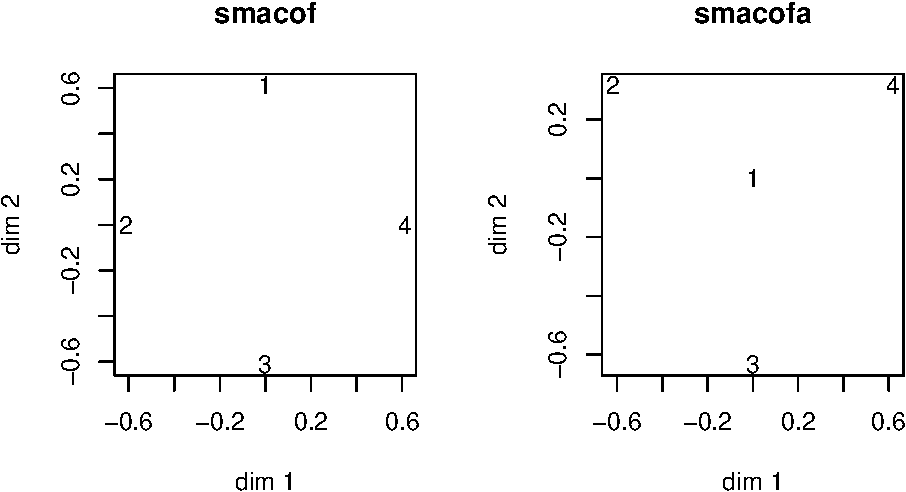
\includegraphics{mSmacof_files/figure-latex/trosmatplot-1.pdf}

\subsection{Ekman}\label{ekman}

We start with the canonical MDS example: average similarity judgments between 14 colors from Ekman (1954).

\begin{Shaded}
\begin{Highlighting}[]
\FunctionTok{data}\NormalTok{(ekman, }\AttributeTok{package =} \StringTok{"smacof"}\NormalTok{)}
\NormalTok{ekman }\OtherTok{\textless{}{-}}\NormalTok{ (}\DecValTok{1} \SpecialCharTok{{-}}\NormalTok{ ekman) }\SpecialCharTok{\^{}} \DecValTok{3}
\NormalTok{hekman }\OtherTok{\textless{}{-}} \FunctionTok{exampleRun}\NormalTok{(ekman)}
\end{Highlighting}
\end{Shaded}

Note that we use power three to compute dissimilarities from the similarities, because previous research has shown that for these transformed dissimilarities \textbf{smacof} in two dimensions computes the global minimum (De Leeuw (2019)). The ekman example is definitely atypical in this respect.

\subsubsection{Results}\label{results-1}

\paragraph{Smacof Meets Newton}\label{smacof-meets-newton-1}

\begin{Shaded}
\begin{Highlighting}[]
\FunctionTok{print}\NormalTok{(hekman}\SpecialCharTok{$}\NormalTok{results, }\AttributeTok{digits =} \DecValTok{10}\NormalTok{)}
\end{Highlighting}
\end{Shaded}

\begin{verbatim}
##              itel         stress         emprate          minhess      time
## smacof         32 0.005512405968 5.357762267e-01  1.998401444e-15  3.772164
## smacofrelax    24 0.005512405968 4.124112181e-01  1.554312234e-15  3.154376
## smacofa       581 0.005512405968 9.645817777e-01  3.541831207e-02 33.523814
## smacofarelax  315 0.005512405968 9.335771478e-01  3.541831208e-02 19.714317
## newton          5 0.005512405968 4.879580532e-07  1.998401444e-15  4.095490
## newtona        10 0.020611324154 2.607932558e-05 -1.737420981e-02  6.258117
## strategy2       7 0.005512405968 1.114331611e-06  1.776356839e-15  4.996096
## strategy2a     76 0.005512405968 4.712405280e-07  3.541831208e-02 39.738102
## strategy3       6 0.005512405968 6.515656134e-07  1.998401444e-15  4.554034
## strategy3a     77 0.005512405968 2.216251231e-07  3.541831208e-02 40.248060
## strategy1-2     6 0.005512405968 1.937624704e-07  2.664535259e-15  3.751418
## strategy1-4    12 0.005512405968 1.482112273e-07  1.554312234e-15  3.623129
## strategy1-6    19 0.005512405968 1.276362317e-06  1.776356839e-15  3.600169
\end{verbatim}

\paragraph{Smacof Quickstep}\label{smacof-quickstep-1}

\begin{Shaded}
\begin{Highlighting}[]
\NormalTok{hsekman }\OtherTok{\textless{}{-}} \FunctionTok{exampleRun2}\NormalTok{(ekman)}
\FunctionTok{print}\NormalTok{(hsekman}\SpecialCharTok{$}\NormalTok{results, }\AttributeTok{digits =} \DecValTok{10}\NormalTok{)}
\end{Highlighting}
\end{Shaded}

\begin{verbatim}
##                          itel         stress     time
## otmax = 1,    nterms = 1    5 0.005512428024 0.894743
## otmax = 5,    nterms = 1    5 0.005512408969 1.095766
## otmax = 10,   nterms = 1    5 0.005512408969 1.089534
## otmax = 100,  nterms = 1    5 0.005512408969 1.252345
## otmax = 1,    nterms = 2    4 0.005512409453 0.950872
## otmax = 5,    nterms = 2    3 0.005512414745 0.919753
## otmax = 10,   nterms = 2    3 0.005512414745 0.944066
## otmax = 100,  nterms = 2    3 0.005512414745 0.916637
## otmax = 1,    nterms = 3    4 0.005512406024 1.156610
## otmax = 5,    nterms = 3    3 0.005512406849 1.114298
## otmax = 10,   nterms = 3    3 0.005512406849 1.114052
## otmax = 100,  nterms = 3    3 0.005512406849 1.113191
## otmax = 1,    nterms = 4    3 0.005512406470 1.106180
## otmax = 5,    nterms = 4    3 0.005512406125 1.246195
## otmax = 10,   nterms = 4    3 0.005512406125 1.398428
## otmax = 100,  nterms = 4    3 0.005512406125 1.569603
\end{verbatim}

\subsubsection{Discussion}\label{discussion}

This small example has a good fit in two dimensions. It can be characterized as very well-behaved and very easy.
All eight strategies give the same solution, which we shall show to be the global minimum.
relaxed \textbf{smacof} takes the least time to converge. Both \textbf{newton}, \textbf{strategy 2}, and
\textbf{strategy 3} are quite competative, being less than a second slower.

The eigenvalues of \(V^+B(\theta)\) at the \textbf{smacof} solution are

\begin{verbatim}
##  [1] +1.000000000023987 +0.999999999953508 +0.923497086335441 +0.907901212921802
##  [5] +0.862936584809353 +0.852692003044618 +0.829803620826543 +0.814556167660674
##  [9] +0.793238576326464 +0.791651722426952 +0.786442678063926 +0.747679475652772
## [13] +0.728268247392202 +0.000000000000001
\end{verbatim}

The fact that the two largest eigenvalues are equal to one verifies that the Gower rank is two, and that the solution is indeed the two-dimensional global minimum (De Leeuw (2016)). Remember this is for the dissimilarities \(\delta_{ij}=(1-s_{ij})^3\). Powering dissimilarities generally decreases the Gower rank (De Leeuw (2023)).

The reduced basis leads to many more iterations, and a much more time-consuming run, compared to the full
basis. It seems that \textbf{smacof} likes the additional freedom of the full basis, and does not like
to be forced into a fixed rotation. We will find this throughout our examples, so there is no need
to point this out every time.

\subsection{Equal Distances}\label{equal-distances}

The next example has 15 objects. All dissimilarities are equal.

\begin{Shaded}
\begin{Highlighting}[]
\NormalTok{equi }\OtherTok{\textless{}{-}} \FunctionTok{oneDist}\NormalTok{(}\DecValTok{15}\NormalTok{)}
\NormalTok{hequi }\OtherTok{\textless{}{-}} \FunctionTok{exampleRun}\NormalTok{(equi)}
\end{Highlighting}
\end{Shaded}

This is a wordt-case example in most respects. The MDS problem is known to have many local minima, mainly because permuting the points of any local minimizer gives other local minimizers with the same stress. Given previous research
(De Leeuw and Stoop (1984)) we think that the global minimum is attained with twelve points
equally spaced on a circle and the remaining three points as corners of an equilateral triangle in the interior of the circle. Which of the 15 points ultimately occupy each of the fifteen possible positions on the circle and triangle is obviously arbitrary.

\subsubsection{Results}\label{results-2}

\paragraph{Smacof Meets Newton}\label{smacof-meets-newton-2}

\begin{verbatim}
##                 itel          stress           emprate            minhess
## smacof        455929 0.0656151291922 9.99987233515e-01  2.99335468054e-16
## smacofrelax   297936 0.0656151291922 9.99957175521e-01  2.79627942445e-15
## smacofa      1000000 0.0656151299341 1.00000081107e+00 -8.12969537114e-07
## smacofarelax 1000000 0.0656151293147 9.99997800055e-01  9.41461513281e-07
## newton            37 0.0670111879007 9.86462255373e-07 -1.66991062323e-01
## newtona          222 0.0661927090396 1.31607436892e-06 -1.49242477209e-01
## strategy2      15728 0.0656151296469 4.53706668312e-05 -1.36764999048e-08
## strategy2a    100000 0.0656151293052 9.99999313529e-01  6.89711689832e-07
## strategy3     100000 0.0656151300845 1.00001247723e+00 -1.24786555312e-05
## strategy3a    100000 0.0656151292282 9.99998806956e-01  1.18985417551e-06
## strategy1-2      182 0.0659016350177 1.13567760436e-05 -4.88435314865e-02
## strategy1-4      381 0.0656151291922 6.71890462374e-04  2.69186786526e-16
## strategy1-6      706 0.0656151291922 9.22109094156e-05  2.67669872779e-16
##                      time
## smacof       27482.396678
## smacofrelax  18411.155985
## smacofa      60446.070687
## smacofarelax 62176.770149
## newton          19.562125
## newtona        115.297453
## strategy2     8815.855219
## strategy2a   53660.499716
## strategy3    55553.805465
## strategy3a   53600.590844
## strategy1-2     31.147495
## strategy1-4     31.108504
## strategy1-6     48.058929
\end{verbatim}

\paragraph{Smacof Quickstep}\label{smacof-quickstep-2}

\begin{Shaded}
\begin{Highlighting}[]
\NormalTok{hsequi }\OtherTok{\textless{}{-}} \FunctionTok{exampleRun2}\NormalTok{(equi)}
\FunctionTok{print}\NormalTok{(hsequi}\SpecialCharTok{$}\NormalTok{results, }\AttributeTok{digits =} \DecValTok{10}\NormalTok{)}
\end{Highlighting}
\end{Shaded}

\begin{verbatim}
##                          itel        stress      time
## otmax = 1,    nterms = 1   94 0.06561750099 14.446596
## otmax = 5,    nterms = 1   64 0.06561691380 11.195009
## otmax = 10,   nterms = 1   62 0.06561692029 11.108909
## otmax = 100,  nterms = 1   62 0.06561691707 11.018176
## otmax = 1,    nterms = 2   91 0.06561594246 16.375769
## otmax = 5,    nterms = 2   76 0.06561592535 17.166044
## otmax = 10,   nterms = 2   67 0.06561595994 16.255803
## otmax = 100,  nterms = 2   68 0.06561591964 17.106922
## otmax = 1,    nterms = 3   75 0.06561555622 17.653821
## otmax = 5,    nterms = 3   64 0.06561554509 17.447304
## otmax = 10,   nterms = 3   63 0.06561552359 19.174675
## otmax = 100,  nterms = 3   63 0.06561552711 19.707798
## otmax = 1,    nterms = 4   70 0.06561539711 20.871255
## otmax = 5,    nterms = 4   66 0.06553507721 22.877713
## otmax = 10,   nterms = 4   38 0.06553491132 17.249643
## otmax = 100,  nterms = 4   32 0.06553492217 18.300514
\end{verbatim}

\subsubsection{Discussion}\label{discussion-1}

This example, though small, is tough, because it has \(\text{factorial}(15)\) local minima, all
with the same function value. The Gower rank is 14, with the points in the
optimal configuration in 14 dimensions on a regular simplex. The fact that
all singular values of the full-dimensional solution are equal indicates
there will be difficulties projecting into two dimensions (think of
the power method with all eigenvalues equal).

Both \textbf{smacof} and \textbf{smacofa} have not converged in 100,000 iterations.
To more clearly distinguish the two, we now set \emph{itmax} equal to 1,000,000 and
run \textbf{smacof} and \textbf{smacofa} again.

The final \textbf{smacof} configuration consists of eleven points equally spaced on a circle
and four points in the corners of a square inside the circle. The final \textbf{smacofa}
configuration is the presumed global minimum with twelve points on the circle and an equilateral triangle within the circle.

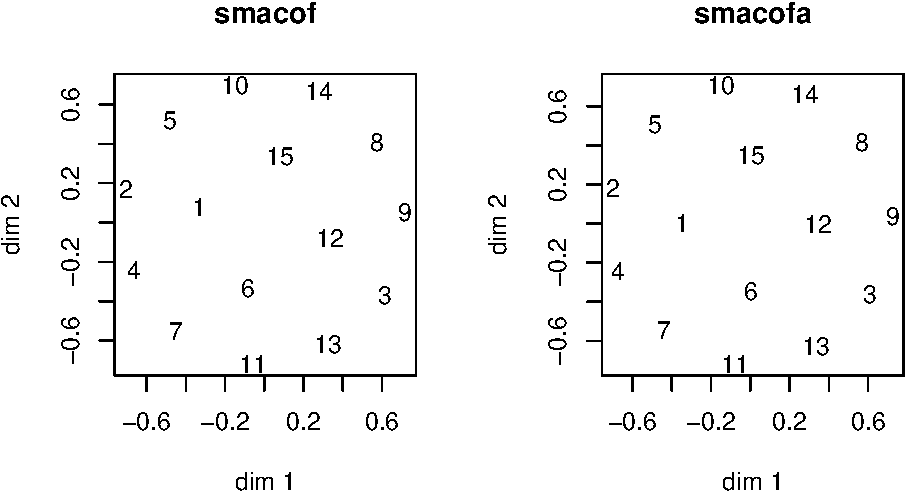
\includegraphics{mSmacof_files/figure-latex/equiplot-1.pdf}

It is not impossible that if we continue iterating then
in the distant future, after life on earth has long disappeared,
eigenvalue 24 will be zero, and the convergence rate will consequently
be one. The only way to be sure is to use study the two configurations
using exact arithmetic to see if eigenvalue 24 is really zero.

Both \textbf{strategy2a} and \textbf{strategy2b} seem to converge to the same stationary value as
\textbf{smacofa}, which is not surprising because they all use the reduced basis.
\textbf{strategy2} and \textbf{strategy3} seem to converge a saddlepoint.

\subsection{Morse}\label{morse}

Next, similarities between 36 morse signals, taken from Rothkopf (1957).

\begin{Shaded}
\begin{Highlighting}[]
\FunctionTok{data}\NormalTok{(morse, }\AttributeTok{package =} \StringTok{"smacof"}\NormalTok{)}
\NormalTok{morse }\OtherTok{\textless{}{-}} \DecValTok{1} \SpecialCharTok{{-}}\NormalTok{ morse}
\NormalTok{hmorse }\OtherTok{\textless{}{-}} \FunctionTok{exampleRun}\NormalTok{(morse)}
\end{Highlighting}
\end{Shaded}

\subsubsection{Results}\label{results-3}

\paragraph{Smacof Meets Newton}\label{smacof-meets-newton-3}

\begin{verbatim}
##               itel       stress         emprate          minhess         time
## smacof         831 0.1760679948 9.676536873e-01 -2.714543931e-15    72.710917
## smacofrelax    450 0.1760679948 9.390097747e-01 -3.265064144e-15    41.688882
## smacofa      94359 0.1765537739 9.998984186e-01  1.013903007e-04  9099.202734
## smacofarelax 50617 0.1765537739 9.997530920e-01  1.013801725e-04  5066.727602
## newton         250 2.3348813599 5.618110024e+00 -1.118156235e-01   543.965245
## newtona        250 0.2041685333 8.073197549e-01 -7.612760274e-01   541.815246
## strategy2      133 0.1769586660 4.703540688e-07 -2.096935642e-15   266.017840
## strategy2a    5169 0.1777018041 8.583657112e-06  6.714577385e-04 11216.130970
## strategy3      280 0.1760679948 9.905927116e-08 -2.857947696e-15   564.867824
## strategy3a    3529 0.1765537739 6.576444715e-05  1.013700413e-04  7678.822596
## strategy1-2     43 0.1765810284 2.023350347e-06 -3.653247388e-15    31.019780
## strategy1-4    371 0.1760679948 9.566240633e-07 -2.800006049e-15    47.325111
## strategy1-6    553 0.1760679948 4.282207201e-06 -2.843573644e-15    55.178087
\end{verbatim}

\paragraph{Smacof Quickstep}\label{smacof-quickstep-3}

\begin{Shaded}
\begin{Highlighting}[]
\NormalTok{hsmorse }\OtherTok{\textless{}{-}} \FunctionTok{exampleRun2}\NormalTok{(morse)}
\FunctionTok{print}\NormalTok{(hsmorse}\SpecialCharTok{$}\NormalTok{results, }\AttributeTok{digits =} \DecValTok{10}\NormalTok{)}
\end{Highlighting}
\end{Shaded}

\begin{verbatim}
##                          itel       stress      time
## otmax = 1,    nterms = 1   73 0.1765127194 15.605461
## otmax = 5,    nterms = 1   62 0.1765127255 21.458539
## otmax = 10,   nterms = 1   62 0.1765127422 21.747835
## otmax = 100,  nterms = 1   62 0.1765127422 22.414700
## otmax = 1,    nterms = 2   53 0.1765123936 19.630349
## otmax = 5,    nterms = 2   37 0.1765123845 19.652858
## otmax = 10,   nterms = 2   35 0.1765123568 20.928040
## otmax = 100,  nterms = 2   34 0.1765123566 21.459277
## otmax = 1,    nterms = 3   43 0.1765122705 20.505617
## otmax = 5,    nterms = 3   33 0.1765122544 21.663457
## otmax = 10,   nterms = 3   30 0.1765122552 22.958688
## otmax = 100,  nterms = 3   28 0.1765122482 23.793120
## otmax = 1,    nterms = 4   37 0.1765122041 22.340285
## otmax = 5,    nterms = 4   30 0.1765122059 24.102875
## otmax = 10,   nterms = 4   28 0.1765121983 26.258491
## otmax = 100,  nterms = 4   28 0.1765122101 28.152732
\end{verbatim}

\subsubsection{Discussion}\label{discussion-2}

\subsection{De Gruijter}\label{de-gruijter}

Similarities between nine Dutch political parties in 1966, taken from De Gruijter (1967).
They were computed by using the complete method of triads, followed by
averaging over a politically heterogeneous group of 100 students.

\begin{Shaded}
\begin{Highlighting}[]
\FunctionTok{source}\NormalTok{(}\StringTok{"gruijter.R"}\NormalTok{)}
\NormalTok{hgruijter }\OtherTok{\textless{}{-}} \FunctionTok{exampleRun}\NormalTok{(gruijter)}
\end{Highlighting}
\end{Shaded}

\subsubsection{Results}\label{results-4}

\paragraph{Smacof Meets Newton}\label{smacof-meets-newton-4}

\begin{verbatim}
##              itel        stress         emprate          minhess       time
## smacof       1117 0.02230169129 9.861521851e-01  3.878130944e-16  60.368933
## smacofrelax   600 0.02230169129 9.730252717e-01 -4.341758314e-16  34.404863
## smacofa      7893 0.02449551136 9.977555156e-01  2.244435229e-03 408.947202
## smacofarelax 4116 0.02449551136 9.955337984e-01  2.244435377e-03 218.617043
## newton         15 0.02857105093 9.134578614e-07 -2.342201358e-01   6.721212
## newtona       125 0.05825528603 3.574317609e-06 -1.614072759e+00  44.457694
## strategy2      43 0.02449551136 1.554811517e-06 -2.389367779e-16  16.356704
## strategy2a   1163 0.02323104236 8.262462508e-07  9.749051769e-04 427.466328
## strategy3      57 0.02230169129 6.740550916e-07  2.557172303e-16  21.331029
## strategy3a   1496 0.02449551136 5.726315696e-08  2.244435525e-03 551.363572
## strategy1-2    79 0.02230169129 3.193405904e-07  6.047477807e-16  14.405596
## strategy1-4   154 0.02230169129 8.886248189e-07  2.702524186e-16  10.699893
## strategy1-6   459 0.02230169129 5.818046455e-06  2.958439331e-16  25.483591
\end{verbatim}

\paragraph{Smacof Quickstep}\label{smacof-quickstep-4}

\begin{Shaded}
\begin{Highlighting}[]
\NormalTok{hsgruijter }\OtherTok{\textless{}{-}} \FunctionTok{exampleRun2}\NormalTok{(gruijter)}
\FunctionTok{print}\NormalTok{(hsgruijter}\SpecialCharTok{$}\NormalTok{results, }\AttributeTok{digits =} \DecValTok{10}\NormalTok{)}
\end{Highlighting}
\end{Shaded}

\begin{verbatim}
##                          itel        stress      time
## otmax = 1,    nterms = 1   57 0.02230297714  6.334746
## otmax = 5,    nterms = 1   47 0.02230297055  9.311920
## otmax = 10,   nterms = 1   46 0.02230297289  9.834055
## otmax = 100,  nterms = 1   46 0.02230293136 10.584560
## otmax = 1,    nterms = 2   45 0.02230221250  7.305626
## otmax = 5,    nterms = 2   32 0.02230224942  7.098658
## otmax = 10,   nterms = 2   31 0.02230222041  8.098033
## otmax = 100,  nterms = 2   30 0.02230223405  8.979287
## otmax = 1,    nterms = 3   38 0.02230197809  7.866055
## otmax = 5,    nterms = 3   30 0.02230199254  8.157237
## otmax = 10,   nterms = 3   28 0.02230197328  9.197776
## otmax = 100,  nterms = 3   27 0.02230197703 10.177512
## otmax = 1,    nterms = 4   33 0.02230187639  8.919222
## otmax = 5,    nterms = 4   27 0.02230188084  8.997081
## otmax = 10,   nterms = 4   25 0.02230188266  9.834506
## otmax = 100,  nterms = 4   24 0.02230188104 11.839529
\end{verbatim}

\subsubsection{Discussion}\label{discussion-3}

\subsection{Trading}\label{trading}

Trading between countries, taken from Cox and Cox (2001)

\begin{Shaded}
\begin{Highlighting}[]
\FunctionTok{data}\NormalTok{(trading, }\AttributeTok{package =} \StringTok{"smacof"}\NormalTok{)}
\NormalTok{htrading }\OtherTok{\textless{}{-}} \FunctionTok{exampleRun}\NormalTok{(trading)}
\end{Highlighting}
\end{Shaded}

\subsubsection{Results}\label{results-5}

\paragraph{Smacof Meets Newton}\label{smacof-meets-newton-5}

\begin{verbatim}
##               itel        stress         emprate          minhess        time
## smacof         757 0.03556267022 9.794532017e-01  6.758230563e-17   50.213561
## smacofrelax    410 0.03556267022 9.604728432e-01 -9.527605636e-16   26.472429
## smacofa      26278 0.03542731412 9.994585067e-01  5.415968766e-04 1740.421136
## smacofarelax 13799 0.03542731412 9.989217979e-01  5.415967289e-04  944.827739
## newton         250 0.07866088391 6.237785912e-01 -4.801794233e-01  167.399228
## newtona        250 0.10315153940 7.577402692e-01 -3.102375743e-01  162.699603
## strategy2       84 0.03556267022 1.621081302e-06 -2.398603457e-18   59.081164
## strategy2a    3357 0.03542731412 2.842514318e-08  5.415965811e-04 2429.942613
## strategy3       84 0.03556267022 1.621081302e-06 -2.398603457e-18   59.925354
## strategy3a    3272 0.03542731412 3.258043371e-07  5.415965811e-04 2339.677259
## strategy1-2    112 0.03555063190 1.296712418e-07 -1.217175791e-01   35.706818
## strategy1-4    118 0.03556267022 9.352528012e-07  5.431747396e-17   11.985899
## strategy1-6    316 0.03556267022 1.063773980e-06  4.546585086e-17   22.157958
\end{verbatim}

\paragraph{Smacof Quickstep}\label{smacof-quickstep-5}

\begin{Shaded}
\begin{Highlighting}[]
\NormalTok{hstrading }\OtherTok{\textless{}{-}} \FunctionTok{exampleRun2}\NormalTok{(trading)}
\FunctionTok{print}\NormalTok{(hstrading}\SpecialCharTok{$}\NormalTok{results, }\AttributeTok{digits =} \DecValTok{10}\NormalTok{)}
\end{Highlighting}
\end{Shaded}

\subsubsection{Discussion}\label{discussion-4}

\subsection{Wish}\label{wish}

Eighteen students rated similarities between
12 nations (Kruskal and Wish (1978), p 31) on a scale from zero to nine. The data are the average similarity ratings, converted to dissimilarities by subtracting them from nine.

\begin{Shaded}
\begin{Highlighting}[]
\FunctionTok{source}\NormalTok{(}\StringTok{"wish.R"}\NormalTok{)}
\NormalTok{hwish }\OtherTok{\textless{}{-}} \FunctionTok{exampleRun}\NormalTok{(wish)}
\end{Highlighting}
\end{Shaded}

\subsubsection{Results}\label{results-6}

\paragraph{Smacof Meets Newton}\label{smacof-meets-newton-6}

\begin{verbatim}
##              itel        stress         emprate          minhess      time
## smacof        432 0.02906376247 9.602005756e-01  2.979562443e-17 25.198190
## smacofrelax   240 0.02906376247 9.259203221e-01 -7.018597772e-16 14.323432
## smacofa       748 0.02895458552 9.719895705e-01  2.801063234e-02 41.363547
## smacofarelax  403 0.02895458552 9.468082086e-01  2.801063226e-02 23.325638
## newton        174 0.08109079232 3.096752359e-05 -3.132519623e-01 74.705731
## newtona       114 0.05876421547 3.635698391e-06 -1.649508203e+00 49.873015
## strategy2      27 0.02906376247 1.536567911e-07 -2.402137809e-16 12.341246
## strategy2a     86 0.02895458552 1.834585579e-06  2.801063217e-02 36.020017
## strategy3      27 0.02906376247 8.235199983e-01 -1.930590976e-16 12.471257
## strategy3a     87 0.02895458552 1.283111535e-06  2.801063217e-02 36.487827
## strategy1-2    39 0.02906376247 1.047673705e-06 -3.352533786e-16  8.530337
## strategy1-4    96 0.02906376247 3.430500455e-07 -2.428458810e-16  8.231570
## strategy1-6   208 0.02906376247 3.792319279e-07 -8.551137900e-17 13.426270
\end{verbatim}

\paragraph{Smacof Quickstep}\label{smacof-quickstep-6}

\begin{Shaded}
\begin{Highlighting}[]
\NormalTok{hswish }\OtherTok{\textless{}{-}} \FunctionTok{exampleRun2}\NormalTok{(wish)}
\FunctionTok{print}\NormalTok{(hswish}\SpecialCharTok{$}\NormalTok{results, }\AttributeTok{digits =} \DecValTok{10}\NormalTok{)}
\end{Highlighting}
\end{Shaded}

\begin{verbatim}
##                          itel        stress     time
## otmax = 1,    nterms = 1   39 0.02906434590 4.573263
## otmax = 5,    nterms = 1   34 0.02906437748 5.873291
## otmax = 10,   nterms = 1   34 0.02906438805 6.316501
## otmax = 100,  nterms = 1   34 0.02906437227 6.372876
## otmax = 1,    nterms = 2   29 0.02906400103 4.918319
## otmax = 5,    nterms = 2   24 0.02906397903 5.444390
## otmax = 10,   nterms = 2   24 0.02906396002 6.292475
## otmax = 100,  nterms = 2   24 0.02906395941 6.612685
## otmax = 1,    nterms = 3   24 0.02906387777 5.390393
## otmax = 5,    nterms = 3   21 0.02906385823 5.826756
## otmax = 10,   nterms = 3   19 0.02906389217 6.489685
## otmax = 100,  nterms = 3   19 0.02906389041 6.697842
## otmax = 1,    nterms = 4   20 0.02906384578 5.653736
## otmax = 5,    nterms = 4   18 0.02906382646 6.266932
## otmax = 10,   nterms = 4   17 0.02906382668 7.063275
## otmax = 100,  nterms = 4   17 0.02906382864 7.982905
\end{verbatim}

\subsubsection{Discussion}\label{discussion-5}

This is small example, with a good fit. There seem to be three different stationary points.
\textbf{newtona} converges to a saddle point. One of the local minima is found by
\textbf{smacofa}, \textbf{newton}, \textbf{strategy 2a}, and \textbf{strategy 3a}. Its stress (for \textbf{newton}) is . The other local minimum is found by
\textbf{smacof}, \textbf{strategy2} and \textbf{strategy 3}. It has a slightly higher stress (for \textbf{smacof}) of . In the two plots the first and ``best'' local minimum is on the
left, the second is on the right. Although the grouping of the nations in the two plots
is similar, their actual locations are quite different.

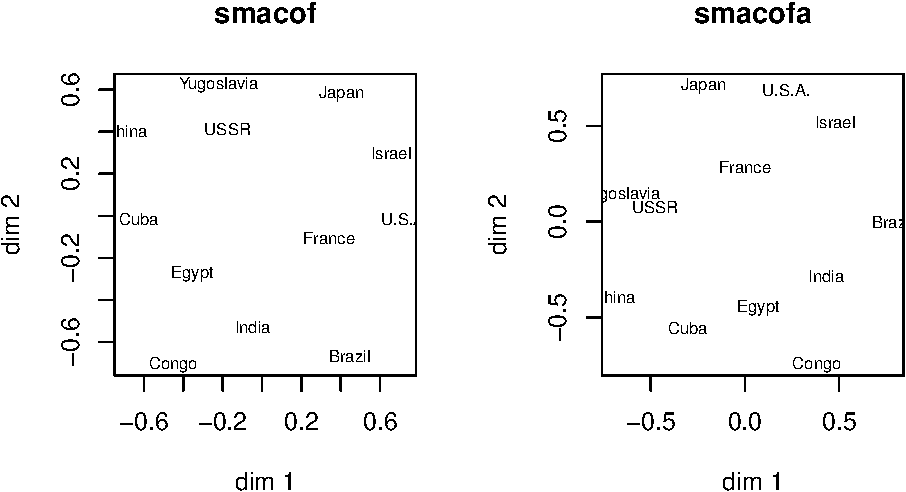
\includegraphics{mSmacof_files/figure-latex/wishplot-1.pdf}

\subsection{Airline Distances}\label{airline-distances}

Airline distances between 18 cities are taken from Izenman (2008), page 466, who collected them from the National Geographic Society's \emph{Atlas of the World}, sixth edition, 1995. Because of the spherical earth the larger distances cannot properly be
projected on the plane, and the MDS will be like a spherical projection.

\begin{Shaded}
\begin{Highlighting}[]
\FunctionTok{source}\NormalTok{(}\StringTok{"airline.R"}\NormalTok{)}
\NormalTok{hairline }\OtherTok{\textless{}{-}} \FunctionTok{exampleRun}\NormalTok{(airline)}
\end{Highlighting}
\end{Shaded}

The cities are Beijing.

\subsubsection{Results}\label{results-7}

\paragraph{Smacof Meets Newton}\label{smacof-meets-newton-7}

\begin{verbatim}
##              itel        stress         emprate         minhess       time
## smacof        297 0.00988993672 9.428533733e-01 1.110223025e-15  18.426999
## smacofrelax   168 0.00988993672 8.964618992e-01 1.332267630e-15  11.814519
## smacofa      1935 0.00988993672 9.916922247e-01 8.307369205e-03 117.761102
## smacofarelax 1024 0.00988993672 9.836464616e-01 8.307369194e-03  65.544486
## newton          9 0.00988993672 1.395947034e-07 2.442490654e-15   7.169752
## newtona         8 0.00988993672 1.953624139e-07 8.307369182e-03   6.679310
## strategy2      10 0.00988993672 5.115172131e-08 1.554312234e-15   7.468560
## strategy2a      9 0.00988993672 3.988699891e-08 8.307369182e-03   6.925515
## strategy3      10 0.00988993672 3.694707637e-07 1.332267630e-15   7.473234
## strategy3a      7 0.00988993672 2.152088807e-06 8.307369182e-03   5.979768
## strategy1-2    13 0.00988993672 1.392805054e-05 2.220446049e-15   6.363938
## strategy1-4    66 0.00988993672 3.756790000e-06 1.332267630e-15   7.639530
## strategy1-6   143 0.00988993672 1.069919901e-06 1.332267630e-15  11.470324
\end{verbatim}

\paragraph{Smacof Quickstep}\label{smacof-quickstep-7}

\begin{Shaded}
\begin{Highlighting}[]
\NormalTok{hsairline }\OtherTok{\textless{}{-}} \FunctionTok{exampleRun2}\NormalTok{(airline)}
\FunctionTok{print}\NormalTok{(hsairline}\SpecialCharTok{$}\NormalTok{results, }\AttributeTok{digits =} \DecValTok{10}\NormalTok{)}
\end{Highlighting}
\end{Shaded}

\begin{verbatim}
##                          itel         stress     time
## otmax = 1,    nterms = 1   25 0.009890391116 3.358802
## otmax = 5,    nterms = 1   24 0.009890366162 3.907177
## otmax = 10,   nterms = 1   24 0.009890366162 4.117466
## otmax = 100,  nterms = 1   24 0.009890366162 3.833049
## otmax = 1,    nterms = 2   20 0.009890072856 3.884791
## otmax = 5,    nterms = 2   17 0.009890074833 4.163591
## otmax = 10,   nterms = 2   17 0.009890073609 4.271462
## otmax = 100,  nterms = 2   17 0.009890073609 4.123247
## otmax = 1,    nterms = 3   16 0.009890022949 4.122427
## otmax = 5,    nterms = 3   14 0.009890013048 4.428902
## otmax = 10,   nterms = 3   14 0.009890002767 4.639232
## otmax = 100,  nterms = 3   14 0.009890004884 4.644562
## otmax = 1,    nterms = 4   14 0.009889981214 4.682733
## otmax = 5,    nterms = 4   13 0.009889972369 4.953169
## otmax = 10,   nterms = 4   12 0.009889984652 5.021926
## otmax = 100,  nterms = 4   12 0.009889984652 5.010815
\end{verbatim}

\subsubsection{Discussion}\label{discussion-6}

\section{General Discussion}\label{general-discussion}

\begin{enumerate}
\def\labelenumi{\arabic{enumi}.}
\tightlist
\item
  MDS may have local minima which are quite different but have very close stress values.
\item
  If the dissimilarities have little variation there tend to be many local minima and
  smacof converges very slowly.
\item
  It is imperative to iterate smacof to (very) high precision.
\item
  The reduced basis may have some theoretical appeal but greatly slows down computation.
\item
  strategy 1 iterates smacof to low precision and then switches to newton. This seems to work
  well, especially for larger examples.
\item
  strategy 2 and 3 require computation of both the smacof and newton update in each iteration.
  This is (maybe too) expensive.
\item
  It is imperative to inspect the eigenvalues of the Hessian at convergence.
\item
  The adaptive version of the relaxed update works well and does approximately
  half the number of iterations.
\item
  The relaxed update \(2\Gamma(\theta)-\theta\) should not be used.
\item
  It is informative to inspect the eigenvalues of \(B(\theta)\) at convergence.
\item
  Since using the full basis for unrestricted MDS is equivalent to
  working with \(x\) in \(\mathbb{R}^{np}\), we may as well not use \(Y\) and \(\theta\)
  if there are no constraints.
\item
  It is informative to compute the full-dimensional MDS solution.
\item
  It is informative to use the Hessian to draw pseudo-confidence ellipses.
\item
  It is a good idea to use more than one of the computational strategies
  outlined in this report on a single data set.
\item
  Using unsafeguarded newton from the start is a bad idea.
\item
  For really large examples iterating smacof to high precision may take
  an eternity.
\item
  smacof always converges to a local minimum, except when started in a
  saddle point. Strategies that mix smacof and newton could end up in
  saddle points.
\end{enumerate}

\section{Appendix: R Code}\label{appendix-r-code}

\subsection{utils.R}\label{utils.r}

\begin{Shaded}
\begin{Highlighting}[]
\CommentTok{\# returns unit vector i of length n}

\NormalTok{ei }\OtherTok{\textless{}{-}} \ControlFlowTok{function}\NormalTok{(i, n) \{}
  \FunctionTok{return}\NormalTok{(}\FunctionTok{ifelse}\NormalTok{(i }\SpecialCharTok{==} \DecValTok{1}\SpecialCharTok{:}\NormalTok{n, }\DecValTok{1}\NormalTok{, }\DecValTok{0}\NormalTok{))}
\NormalTok{\}}

\CommentTok{\# return distancing matrix (i,j) of order n}

\NormalTok{aij }\OtherTok{\textless{}{-}} \ControlFlowTok{function}\NormalTok{(i, j, n) \{}
\NormalTok{  df }\OtherTok{\textless{}{-}} \FunctionTok{ei}\NormalTok{(i, n) }\SpecialCharTok{{-}} \FunctionTok{ei}\NormalTok{(j, n)}
  \FunctionTok{return}\NormalTok{(}\FunctionTok{outer}\NormalTok{(df, df))}
\NormalTok{\}}

\CommentTok{\# y is a list of matrices}
\CommentTok{\# returns a matrix with the direct sum of the y[[i]]}

\NormalTok{directSum }\OtherTok{\textless{}{-}} \ControlFlowTok{function}\NormalTok{(y) \{}
\NormalTok{  mr }\OtherTok{\textless{}{-}} \FunctionTok{sum}\NormalTok{(}\FunctionTok{sapply}\NormalTok{(y, nrow))}
\NormalTok{  mc }\OtherTok{\textless{}{-}} \FunctionTok{sum}\NormalTok{(}\FunctionTok{sapply}\NormalTok{(y, ncol))}
\NormalTok{  nr }\OtherTok{\textless{}{-}} \FunctionTok{c}\NormalTok{(}\DecValTok{0}\NormalTok{, }\FunctionTok{cumsum}\NormalTok{(}\FunctionTok{sapply}\NormalTok{(y, nrow)))}
\NormalTok{  nc }\OtherTok{\textless{}{-}} \FunctionTok{c}\NormalTok{(}\DecValTok{0}\NormalTok{, }\FunctionTok{cumsum}\NormalTok{(}\FunctionTok{sapply}\NormalTok{(y, ncol)))}
\NormalTok{  p }\OtherTok{\textless{}{-}} \FunctionTok{length}\NormalTok{(y)}
\NormalTok{  z }\OtherTok{\textless{}{-}} \FunctionTok{matrix}\NormalTok{(}\DecValTok{0}\NormalTok{, mr, mc)}
  \ControlFlowTok{for}\NormalTok{ (i }\ControlFlowTok{in} \DecValTok{1}\SpecialCharTok{:}\NormalTok{p) \{}
\NormalTok{    ind }\OtherTok{\textless{}{-}}\NormalTok{ (nr[i] }\SpecialCharTok{+} \DecValTok{1}\NormalTok{)}\SpecialCharTok{:}\NormalTok{nr[i }\SpecialCharTok{+} \DecValTok{1}\NormalTok{]}
\NormalTok{    jnd }\OtherTok{\textless{}{-}}\NormalTok{ (nc[i] }\SpecialCharTok{+} \DecValTok{1}\NormalTok{)}\SpecialCharTok{:}\NormalTok{nc[i }\SpecialCharTok{+} \DecValTok{1}\NormalTok{]}
\NormalTok{    z[ind, jnd] }\OtherTok{\textless{}{-}}\NormalTok{ y[[i]]}
\NormalTok{  \}}
  \FunctionTok{return}\NormalTok{(z)}
\NormalTok{\}}

\CommentTok{\# y is a matrix}
\CommentTok{\# returns a matrix with the direct sum of p copies of y}

\NormalTok{directExpand }\OtherTok{\textless{}{-}} \ControlFlowTok{function}\NormalTok{(y, p) \{}
  \FunctionTok{return}\NormalTok{(}\FunctionTok{directSum}\NormalTok{(}\FunctionTok{rep}\NormalTok{(}\FunctionTok{list}\NormalTok{(y), p)))}
\NormalTok{\}}

\CommentTok{\# double centers a symmetric matrix}

\NormalTok{doubleCenter }\OtherTok{\textless{}{-}} \ControlFlowTok{function}\NormalTok{(x) \{}
\NormalTok{  rs }\OtherTok{\textless{}{-}} \FunctionTok{apply}\NormalTok{(x, }\DecValTok{1}\NormalTok{, mean)}
\NormalTok{  ss }\OtherTok{\textless{}{-}} \FunctionTok{mean}\NormalTok{(x)}
  \FunctionTok{return}\NormalTok{(x }\SpecialCharTok{{-}} \FunctionTok{outer}\NormalTok{(rs, rs, }\StringTok{"+"}\NormalTok{) }\SpecialCharTok{+}\NormalTok{ ss)}
\NormalTok{\}}

\CommentTok{\# mPrint() formats a matrix (or vector, or scalar) of numbers}
\CommentTok{\# for printing }

\NormalTok{mPrint }\OtherTok{\textless{}{-}} \ControlFlowTok{function}\NormalTok{(x,}
                   \AttributeTok{digits =} \DecValTok{6}\NormalTok{,}
                   \AttributeTok{width =} \DecValTok{8}\NormalTok{,}
                   \AttributeTok{format =} \StringTok{"f"}\NormalTok{,}
                   \AttributeTok{flag =} \StringTok{"+"}\NormalTok{) \{}
  \FunctionTok{print}\NormalTok{(}\FunctionTok{noquote}\NormalTok{(}
    \FunctionTok{formatC}\NormalTok{(}
\NormalTok{      x,}
      \AttributeTok{digits =}\NormalTok{ digits,}
      \AttributeTok{width =}\NormalTok{ width,}
      \AttributeTok{format =}\NormalTok{ format,}
      \AttributeTok{flag =}\NormalTok{ flag}
\NormalTok{    )}
\NormalTok{  ))}
\NormalTok{\}}

\CommentTok{\# classical MDS}

\NormalTok{torgerson }\OtherTok{\textless{}{-}} \ControlFlowTok{function}\NormalTok{(delta, }\AttributeTok{p =} \DecValTok{2}\NormalTok{) \{}
\NormalTok{  e }\OtherTok{\textless{}{-}} \FunctionTok{eigen}\NormalTok{(}\SpecialCharTok{{-}}\NormalTok{.}\DecValTok{5} \SpecialCharTok{*} \FunctionTok{doubleCenter}\NormalTok{(}\FunctionTok{as.matrix}\NormalTok{(delta) }\SpecialCharTok{\^{}} \DecValTok{2}\NormalTok{))}
\NormalTok{  l }\OtherTok{\textless{}{-}} \FunctionTok{sqrt}\NormalTok{(}\FunctionTok{pmax}\NormalTok{(}\DecValTok{0}\NormalTok{, e}\SpecialCharTok{$}\NormalTok{values[}\DecValTok{1}\SpecialCharTok{:}\NormalTok{p]))}
  \ControlFlowTok{if}\NormalTok{ (p }\SpecialCharTok{==} \DecValTok{1}\NormalTok{) \{}
    \FunctionTok{return}\NormalTok{(}\FunctionTok{as.matrix}\NormalTok{(e}\SpecialCharTok{$}\NormalTok{vectors[, }\DecValTok{1}\NormalTok{] }\SpecialCharTok{*}\NormalTok{ l))}
\NormalTok{  \} }\ControlFlowTok{else}\NormalTok{ \{}
    \FunctionTok{return}\NormalTok{(e}\SpecialCharTok{$}\NormalTok{vectors[, }\DecValTok{1}\SpecialCharTok{:}\NormalTok{p] }\SpecialCharTok{\%*\%} \FunctionTok{diag}\NormalTok{(l))}
\NormalTok{  \}}
\NormalTok{\}}

\CommentTok{\# converts dist object w to M{-}matrix}

\NormalTok{mmatrix }\OtherTok{\textless{}{-}} \ControlFlowTok{function}\NormalTok{(w) \{}
\NormalTok{  v }\OtherTok{\textless{}{-}} \SpecialCharTok{{-}}\FunctionTok{as.matrix}\NormalTok{(w)}
  \FunctionTok{diag}\NormalTok{(v) }\OtherTok{\textless{}{-}} \SpecialCharTok{{-}}\FunctionTok{rowSums}\NormalTok{(v)}
  \FunctionTok{return}\NormalTok{(v)}
\NormalTok{\}}

\CommentTok{\# create dist with all elements equal to one}

\NormalTok{oneDist }\OtherTok{\textless{}{-}} \ControlFlowTok{function}\NormalTok{(n) \{}
  \FunctionTok{return}\NormalTok{(}\FunctionTok{as.dist}\NormalTok{(}\FunctionTok{matrix}\NormalTok{(}\DecValTok{1}\NormalTok{, n, n)))}
\NormalTok{\}}

\DocumentationTok{\#\# partitioned matrix to single matrix}

\NormalTok{par2mat }\OtherTok{\textless{}{-}} \ControlFlowTok{function}\NormalTok{(x) \{}
\NormalTok{  nc }\OtherTok{\textless{}{-}} \FunctionTok{length}\NormalTok{(x[[}\DecValTok{1}\NormalTok{]])}
\NormalTok{  nr }\OtherTok{\textless{}{-}} \FunctionTok{length}\NormalTok{(x)}
\NormalTok{  h }\OtherTok{\textless{}{-}} \ConstantTok{NULL}
  \ControlFlowTok{for}\NormalTok{ (i }\ControlFlowTok{in} \DecValTok{1}\SpecialCharTok{:}\NormalTok{nr) \{}
\NormalTok{    hi }\OtherTok{\textless{}{-}} \ConstantTok{NULL}
    \ControlFlowTok{for}\NormalTok{ (j }\ControlFlowTok{in} \DecValTok{1}\SpecialCharTok{:}\NormalTok{nc) \{}
\NormalTok{      hi }\OtherTok{\textless{}{-}} \FunctionTok{cbind}\NormalTok{(hi, x[[i]][[j]])}
\NormalTok{    \}}
\NormalTok{    h }\OtherTok{\textless{}{-}} \FunctionTok{rbind}\NormalTok{(h, hi)}
\NormalTok{  \}}
  \FunctionTok{return}\NormalTok{(h)}
\NormalTok{\}}

\CommentTok{\# vector to partitioned list, inverse of unlist()}

\NormalTok{vec2List }\OtherTok{\textless{}{-}} \ControlFlowTok{function}\NormalTok{(x, y) \{}
\NormalTok{  z }\OtherTok{\textless{}{-}} \FunctionTok{list}\NormalTok{()}
\NormalTok{  h }\OtherTok{\textless{}{-}} \FunctionTok{sapply}\NormalTok{(y, ncol)}
\NormalTok{  p }\OtherTok{\textless{}{-}} \FunctionTok{length}\NormalTok{(h)}
\NormalTok{  ind }\OtherTok{\textless{}{-}} \FunctionTok{cumsum}\NormalTok{(}\FunctionTok{c}\NormalTok{(}\DecValTok{1}\NormalTok{, h))[}\SpecialCharTok{{-}}\NormalTok{(p }\SpecialCharTok{+} \DecValTok{1}\NormalTok{)]}
\NormalTok{  jnd }\OtherTok{\textless{}{-}}\NormalTok{ ind }\SpecialCharTok{+}\NormalTok{ (h }\SpecialCharTok{{-}} \DecValTok{1}\NormalTok{)}
  \ControlFlowTok{for}\NormalTok{ (k }\ControlFlowTok{in} \DecValTok{1}\SpecialCharTok{:}\NormalTok{p) \{}
\NormalTok{    z }\OtherTok{\textless{}{-}} \FunctionTok{c}\NormalTok{(z, }\FunctionTok{list}\NormalTok{(x[ind[k]}\SpecialCharTok{:}\NormalTok{jnd[k]]))}
\NormalTok{  \}}
  \FunctionTok{return}\NormalTok{(z)}
\NormalTok{\}}

\CommentTok{\# tmForm of a matrix X has x\_\{ij\}=0 if j geq i}
\CommentTok{\# while the distances satisfy D(tlForm(X)) = D(X)}

\NormalTok{tmForm }\OtherTok{\textless{}{-}} \ControlFlowTok{function}\NormalTok{(x) \{}
\NormalTok{  x }\OtherTok{\textless{}{-}}\NormalTok{ x }\SpecialCharTok{{-}} \FunctionTok{matrix}\NormalTok{(x[}\DecValTok{1}\NormalTok{,], }\FunctionTok{nrow}\NormalTok{(x), }\FunctionTok{ncol}\NormalTok{(x), }\AttributeTok{byrow =} \ConstantTok{TRUE}\NormalTok{)}
\NormalTok{  x[}\SpecialCharTok{{-}}\DecValTok{1}\NormalTok{,] }\OtherTok{\textless{}{-}}\NormalTok{ x[}\SpecialCharTok{{-}}\DecValTok{1}\NormalTok{,] }\SpecialCharTok{\%*\%} \FunctionTok{qr.Q}\NormalTok{(}\FunctionTok{qr}\NormalTok{(}\FunctionTok{t}\NormalTok{(x[}\SpecialCharTok{{-}}\DecValTok{1}\NormalTok{,])))}
  \FunctionTok{return}\NormalTok{(x)}
\NormalTok{\}}

\CommentTok{\# dlForm of a matrix X has e\textquotesingle{}X = 0 and x\_\{ij\}=0 if j \textgreater{} i}
\CommentTok{\# while the distances satisfy D(dlForm(X)) = D(X)}

\NormalTok{dlForm }\OtherTok{\textless{}{-}} \ControlFlowTok{function}\NormalTok{(x) \{}
\NormalTok{  x }\OtherTok{\textless{}{-}} \FunctionTok{apply}\NormalTok{(x, }\DecValTok{2}\NormalTok{, }\ControlFlowTok{function}\NormalTok{(x)}
\NormalTok{    x }\SpecialCharTok{{-}} \FunctionTok{mean}\NormalTok{(x))}
  \FunctionTok{return}\NormalTok{(x }\SpecialCharTok{\%*\%} \FunctionTok{qr.Q}\NormalTok{(}\FunctionTok{qr}\NormalTok{(}\FunctionTok{t}\NormalTok{(x))))}
\NormalTok{\}}

\CommentTok{\# returns a configuration scaled to minimize stress}

\NormalTok{scalConf }\OtherTok{\textless{}{-}} \ControlFlowTok{function}\NormalTok{(delta, x, }\AttributeTok{w =} \FunctionTok{oneDist}\NormalTok{(}\FunctionTok{attr}\NormalTok{(delta, }\StringTok{"Size"}\NormalTok{))) \{}
\NormalTok{  d }\OtherTok{\textless{}{-}} \FunctionTok{dist}\NormalTok{(x)}
\NormalTok{  lbd }\OtherTok{\textless{}{-}} \FunctionTok{sum}\NormalTok{(w }\SpecialCharTok{*}\NormalTok{ delta }\SpecialCharTok{*}\NormalTok{ d) }\SpecialCharTok{/} \FunctionTok{sum}\NormalTok{(w }\SpecialCharTok{*}\NormalTok{ (d }\SpecialCharTok{\^{}} \DecValTok{2}\NormalTok{))}
  \FunctionTok{return}\NormalTok{(lbd }\SpecialCharTok{*}\NormalTok{ x)}
\NormalTok{\}}

\CommentTok{\# just returns stress}

\NormalTok{stressComp }\OtherTok{\textless{}{-}} \ControlFlowTok{function}\NormalTok{(delta, x, }\AttributeTok{w =} \FunctionTok{oneDist}\NormalTok{(}\FunctionTok{attr}\NormalTok{(delta, }\StringTok{"Size"}\NormalTok{))) \{}
  \FunctionTok{return}\NormalTok{(}\FunctionTok{sum}\NormalTok{(w }\SpecialCharTok{*}\NormalTok{ (delta }\SpecialCharTok{{-}} \FunctionTok{dist}\NormalTok{(x)) }\SpecialCharTok{\^{}} \DecValTok{2}\NormalTok{) }\SpecialCharTok{/} \DecValTok{2}\NormalTok{)}
\NormalTok{\}}

\CommentTok{\# returns a weighted sum of matrices in a list x with weights in a}

\NormalTok{listSum }\OtherTok{\textless{}{-}} \ControlFlowTok{function}\NormalTok{(x, }\AttributeTok{a =} \FunctionTok{rep}\NormalTok{(}\DecValTok{1}\NormalTok{, }\FunctionTok{length}\NormalTok{(x))) \{}
\NormalTok{  n }\OtherTok{\textless{}{-}} \FunctionTok{length}\NormalTok{(x)}
\NormalTok{  y }\OtherTok{\textless{}{-}} \FunctionTok{array}\NormalTok{(}\DecValTok{0}\NormalTok{, }\FunctionTok{dim}\NormalTok{(x[[}\DecValTok{1}\NormalTok{]]))}
  \ControlFlowTok{for}\NormalTok{ (i }\ControlFlowTok{in} \DecValTok{1}\SpecialCharTok{:}\NormalTok{n) \{}
\NormalTok{    y }\OtherTok{\textless{}{-}}\NormalTok{ y }\SpecialCharTok{+}\NormalTok{ a[i] }\SpecialCharTok{*}\NormalTok{ x[[i]]}
\NormalTok{  \}}
  \FunctionTok{return}\NormalTok{(y)}
\NormalTok{\}}

\NormalTok{guttman }\OtherTok{\textless{}{-}} \ControlFlowTok{function}\NormalTok{(delta, x, }\AttributeTok{w =} \FunctionTok{oneDist}\NormalTok{(}\FunctionTok{nrow}\NormalTok{(x))) \{}
\NormalTok{  v }\OtherTok{\textless{}{-}} \FunctionTok{mmatrix}\NormalTok{(w)}
\NormalTok{  b }\OtherTok{\textless{}{-}} \FunctionTok{mmatrix}\NormalTok{(w }\SpecialCharTok{*}\NormalTok{ delta }\SpecialCharTok{/} \FunctionTok{dist}\NormalTok{(x))}
  \FunctionTok{return}\NormalTok{(}\FunctionTok{solve}\NormalTok{(v }\SpecialCharTok{+} \DecValTok{1}\NormalTok{, b }\SpecialCharTok{\%*\%}\NormalTok{ x))}
\NormalTok{\}}
\end{Highlighting}
\end{Shaded}

\subsection{basis.R}\label{basis.r}

\begin{Shaded}
\begin{Highlighting}[]
\NormalTok{aTriBas }\OtherTok{\textless{}{-}} \ControlFlowTok{function}\NormalTok{(n, p) \{}
\NormalTok{  np }\OtherTok{\textless{}{-}}\NormalTok{ n }\SpecialCharTok{{-}}\NormalTok{ (p }\SpecialCharTok{{-}} \DecValTok{1}\NormalTok{)}
\NormalTok{  x }\OtherTok{\textless{}{-}} \FunctionTok{diag}\NormalTok{(np)}
\NormalTok{  x[, }\DecValTok{1}\NormalTok{] }\OtherTok{\textless{}{-}} \DecValTok{1}
\NormalTok{  x }\OtherTok{\textless{}{-}} \FunctionTok{rbind}\NormalTok{(}\FunctionTok{matrix}\NormalTok{(}\DecValTok{0}\NormalTok{, p }\SpecialCharTok{{-}} \DecValTok{1}\NormalTok{, np), x)}
  \FunctionTok{return}\NormalTok{(}\FunctionTok{qr.Q}\NormalTok{(}\FunctionTok{qr}\NormalTok{(x))[, }\SpecialCharTok{{-}}\DecValTok{1}\NormalTok{, }\AttributeTok{drop =} \ConstantTok{FALSE}\NormalTok{])}
\NormalTok{\}}

\NormalTok{aBasis }\OtherTok{\textless{}{-}} \ControlFlowTok{function}\NormalTok{(n, p) \{}
  \FunctionTok{return}\NormalTok{(}\FunctionTok{lapply}\NormalTok{(}\DecValTok{1}\SpecialCharTok{:}\NormalTok{p, }\ControlFlowTok{function}\NormalTok{(s)}
    \FunctionTok{aTriBas}\NormalTok{(n, s)))}
\NormalTok{\}}

\NormalTok{bFulBas }\OtherTok{\textless{}{-}} \ControlFlowTok{function}\NormalTok{(n) \{}
\NormalTok{  x }\OtherTok{\textless{}{-}} \FunctionTok{diag}\NormalTok{(n)}
\NormalTok{  x[, }\DecValTok{1}\NormalTok{] }\OtherTok{\textless{}{-}} \DecValTok{1}
  \FunctionTok{return}\NormalTok{(}\FunctionTok{qr.Q}\NormalTok{(}\FunctionTok{qr}\NormalTok{(x))[, }\SpecialCharTok{{-}}\DecValTok{1}\NormalTok{])}
\NormalTok{\}}

\NormalTok{bBasis }\OtherTok{\textless{}{-}} \ControlFlowTok{function}\NormalTok{(n, p) \{}
\NormalTok{  x }\OtherTok{\textless{}{-}} \FunctionTok{bFulBas}\NormalTok{(n)}
  \FunctionTok{return}\NormalTok{(}\FunctionTok{lapply}\NormalTok{(}\DecValTok{1}\SpecialCharTok{:}\NormalTok{p, }\ControlFlowTok{function}\NormalTok{(s)}
\NormalTok{    x))}
\NormalTok{\}}

\NormalTok{uBasis }\OtherTok{\textless{}{-}} \ControlFlowTok{function}\NormalTok{(n, p) \{}
\NormalTok{  x }\OtherTok{\textless{}{-}} \FunctionTok{bBasis}\NormalTok{(n, p)}
  \ControlFlowTok{for}\NormalTok{ (i }\ControlFlowTok{in} \DecValTok{1}\SpecialCharTok{:}\NormalTok{n) \{}
\NormalTok{    ei }\OtherTok{\textless{}{-}} \FunctionTok{ifelse}\NormalTok{(i }\SpecialCharTok{==} \DecValTok{1}\SpecialCharTok{:}\NormalTok{n, }\DecValTok{1}\NormalTok{, }\DecValTok{0}\NormalTok{)}
\NormalTok{    ei }\OtherTok{\textless{}{-}} \FunctionTok{as.matrix}\NormalTok{(ei }\SpecialCharTok{{-}} \FunctionTok{mean}\NormalTok{(ei))}
\NormalTok{    x }\OtherTok{\textless{}{-}} \FunctionTok{c}\NormalTok{(x, }\FunctionTok{list}\NormalTok{(ei))}
\NormalTok{  \}}
  \FunctionTok{return}\NormalTok{(x)}
\NormalTok{\}}

\NormalTok{makeBasis }\OtherTok{\textless{}{-}} \ControlFlowTok{function}\NormalTok{(p, basis, w) \{}
\NormalTok{  v }\OtherTok{\textless{}{-}} \FunctionTok{mmatrix}\NormalTok{(w)}
\NormalTok{  n }\OtherTok{\textless{}{-}} \FunctionTok{nrow}\NormalTok{(v)}
\NormalTok{  y }\OtherTok{\textless{}{-}}
    \ControlFlowTok{switch}\NormalTok{(basis,}
           \AttributeTok{A =} \FunctionTok{aBasis}\NormalTok{(n, p),}
           \AttributeTok{B =} \FunctionTok{bBasis}\NormalTok{(n, p),}
           \AttributeTok{C =} \FunctionTok{cBasis}\NormalTok{(n, p))}
\NormalTok{  ev }\OtherTok{\textless{}{-}}
    \FunctionTok{lapply}\NormalTok{(}\DecValTok{1}\SpecialCharTok{:}\NormalTok{p, }\ControlFlowTok{function}\NormalTok{(s)}
      \FunctionTok{eigen}\NormalTok{(}\FunctionTok{crossprod}\NormalTok{(y[[s]], v }\SpecialCharTok{\%*\%}\NormalTok{ y[[s]])))}
\NormalTok{  y }\OtherTok{\textless{}{-}}
    \FunctionTok{lapply}\NormalTok{(}\DecValTok{1}\SpecialCharTok{:}\NormalTok{p, }\ControlFlowTok{function}\NormalTok{(s)}
\NormalTok{      y[[s]] }\SpecialCharTok{\%*\%}\NormalTok{ ev[[s]]}\SpecialCharTok{$}\NormalTok{vectors }\SpecialCharTok{\%*\%} \FunctionTok{diag}\NormalTok{(}\DecValTok{1} \SpecialCharTok{/} \FunctionTok{sqrt}\NormalTok{(ev[[s]]}\SpecialCharTok{$}\NormalTok{values)))}
  \FunctionTok{return}\NormalTok{(y)}
\NormalTok{\}}
\end{Highlighting}
\end{Shaded}

\subsection{derivatives.R}\label{derivatives.r}

\begin{Shaded}
\begin{Highlighting}[]
\CommentTok{\# returns the gradient of stress at X as n x p matrix}

\NormalTok{gradientx }\OtherTok{\textless{}{-}} \ControlFlowTok{function}\NormalTok{(x, b, v) \{}
  \FunctionTok{return}\NormalTok{((v }\SpecialCharTok{{-}}\NormalTok{ b) }\SpecialCharTok{\%*\%}\NormalTok{ x)}
\NormalTok{\}}

\CommentTok{\# returns the gradient of stress at theta as list of vectors}

\NormalTok{gradientt }\OtherTok{\textless{}{-}} \ControlFlowTok{function}\NormalTok{(x, b, v, y) \{}
\NormalTok{  gradx }\OtherTok{\textless{}{-}} \FunctionTok{gradientx}\NormalTok{(x, b, v)}
  \FunctionTok{return}\NormalTok{(}\FunctionTok{lapply}\NormalTok{(}\DecValTok{1}\SpecialCharTok{:}\FunctionTok{length}\NormalTok{(y), }\ControlFlowTok{function}\NormalTok{(s) }\FunctionTok{drop}\NormalTok{(}\FunctionTok{crossprod}\NormalTok{(y[[s]], gradx[, s]))))}
\NormalTok{\}}

\CommentTok{\# returns the Guttman transform at x as matrix}

\NormalTok{guttmanx }\OtherTok{\textless{}{-}} \ControlFlowTok{function}\NormalTok{ (x, b, vinv) \{}
  \FunctionTok{return}\NormalTok{(vinv }\SpecialCharTok{\%*\%}\NormalTok{ b }\SpecialCharTok{\%*\%}\NormalTok{ x)}
\NormalTok{\}}

\CommentTok{\# returns the Guttman transform at theta as list of vectors}

\NormalTok{guttmant }\OtherTok{\textless{}{-}} \ControlFlowTok{function}\NormalTok{(x, b, vinv, y) \{}
\NormalTok{  guttx }\OtherTok{\textless{}{-}} \FunctionTok{guttmanx}\NormalTok{(x, b, vinv)}
  \FunctionTok{return}\NormalTok{(}\FunctionTok{lapply}\NormalTok{(}\DecValTok{1}\SpecialCharTok{:}\FunctionTok{length}\NormalTok{(y), }\ControlFlowTok{function}\NormalTok{(s) }\FunctionTok{drop}\NormalTok{(}\FunctionTok{crossprod}\NormalTok{(y[[s]], guttx[, s]))))}
\NormalTok{\}}

\CommentTok{\# returns the hessian of stress at x as partioned matrix}

\NormalTok{hessianx }\OtherTok{\textless{}{-}} \ControlFlowTok{function}\NormalTok{(x, delta, w) \{}
\NormalTok{  p }\OtherTok{\textless{}{-}} \FunctionTok{ncol}\NormalTok{(x)}
\NormalTok{  n }\OtherTok{\textless{}{-}} \FunctionTok{nrow}\NormalTok{(x)}
\NormalTok{  d }\OtherTok{\textless{}{-}} \FunctionTok{dist}\NormalTok{(x)}
\NormalTok{  aux1 }\OtherTok{\textless{}{-}}\NormalTok{ w }\SpecialCharTok{*}\NormalTok{ delta }\SpecialCharTok{/}\NormalTok{ d}
\NormalTok{  aux2 }\OtherTok{\textless{}{-}}\NormalTok{ w }\SpecialCharTok{*}\NormalTok{ delta }\SpecialCharTok{/}\NormalTok{ (d }\SpecialCharTok{\^{}} \DecValTok{3}\NormalTok{)}
\NormalTok{  hesx }\OtherTok{\textless{}{-}} \FunctionTok{list}\NormalTok{()}
  \ControlFlowTok{for}\NormalTok{ (s }\ControlFlowTok{in} \DecValTok{1}\SpecialCharTok{:}\NormalTok{p) \{}
\NormalTok{    hessrows }\OtherTok{\textless{}{-}} \FunctionTok{list}\NormalTok{()}
\NormalTok{    di }\OtherTok{\textless{}{-}} \FunctionTok{as.dist}\NormalTok{(}\FunctionTok{outer}\NormalTok{(x[, s], x[, s], }\StringTok{"{-}"}\NormalTok{))}
    \ControlFlowTok{for}\NormalTok{ (t }\ControlFlowTok{in} \DecValTok{1}\SpecialCharTok{:}\NormalTok{p) \{}
\NormalTok{      dj }\OtherTok{\textless{}{-}} \FunctionTok{as.dist}\NormalTok{(}\FunctionTok{outer}\NormalTok{(x[, t], x[, t], }\StringTok{"{-}"}\NormalTok{))}
\NormalTok{      hesspart }\OtherTok{\textless{}{-}} \FunctionTok{mmatrix}\NormalTok{(aux2 }\SpecialCharTok{*}\NormalTok{ di }\SpecialCharTok{*}\NormalTok{ dj)}
      \ControlFlowTok{if}\NormalTok{ (s }\SpecialCharTok{==}\NormalTok{ t) \{}
\NormalTok{        hesspart }\OtherTok{\textless{}{-}} \FunctionTok{mmatrix}\NormalTok{(w) }\SpecialCharTok{{-}}\NormalTok{ (}\FunctionTok{mmatrix}\NormalTok{(aux1) }\SpecialCharTok{{-}}\NormalTok{ hesspart)}
\NormalTok{      \}}
\NormalTok{      hessrows }\OtherTok{\textless{}{-}} \FunctionTok{c}\NormalTok{(hessrows, }\FunctionTok{list}\NormalTok{(hesspart))}
\NormalTok{    \}}
\NormalTok{    hesx }\OtherTok{\textless{}{-}} \FunctionTok{c}\NormalTok{(hesx, }\FunctionTok{list}\NormalTok{(hessrows))}
\NormalTok{  \}}
  \FunctionTok{return}\NormalTok{(hesx)}
\NormalTok{\}}

\CommentTok{\# returns the hessian of stress at theta as partioned matrix}

\NormalTok{hessiant }\OtherTok{\textless{}{-}} \ControlFlowTok{function}\NormalTok{(x, delta, w, y) \{}
\NormalTok{  hesx }\OtherTok{\textless{}{-}} \FunctionTok{hessianx}\NormalTok{(x, delta, w)}
\NormalTok{  hest }\OtherTok{\textless{}{-}}\NormalTok{ hesx}
\NormalTok{  p }\OtherTok{\textless{}{-}} \FunctionTok{length}\NormalTok{(y)}
  \ControlFlowTok{for}\NormalTok{ (s }\ControlFlowTok{in} \DecValTok{1}\SpecialCharTok{:}\NormalTok{p) \{}
    \ControlFlowTok{for}\NormalTok{ (t }\ControlFlowTok{in} \DecValTok{1}\SpecialCharTok{:}\NormalTok{p) \{}
\NormalTok{      hest[[s]][[t]] }\OtherTok{\textless{}{-}} \FunctionTok{crossprod}\NormalTok{(y[[s]], (hesx[[s]][[t]] }\SpecialCharTok{\%*\%}\NormalTok{ y[[t]]))}
\NormalTok{    \}}
\NormalTok{  \}}
  \FunctionTok{return}\NormalTok{(hest)}
\NormalTok{\}}


\CommentTok{\# computes first, second, and third derivatives (in x space for now).}

\NormalTok{thirdx }\OtherTok{\textless{}{-}} \ControlFlowTok{function}\NormalTok{(delta, x, }\AttributeTok{w =} \DecValTok{1} \SpecialCharTok{{-}} \FunctionTok{diag}\NormalTok{(}\FunctionTok{nrow}\NormalTok{(x))) \{}
\NormalTok{  n }\OtherTok{\textless{}{-}} \FunctionTok{nrow}\NormalTok{(x)}
\NormalTok{  p }\OtherTok{\textless{}{-}} \FunctionTok{ncol}\NormalTok{(x)}
\NormalTok{  np }\OtherTok{\textless{}{-}}\NormalTok{ n }\SpecialCharTok{*}\NormalTok{ p}
\NormalTok{  w }\OtherTok{\textless{}{-}} \DecValTok{2} \SpecialCharTok{*}\NormalTok{ w }\SpecialCharTok{/} \FunctionTok{sum}\NormalTok{(w)}
\NormalTok{  delta }\OtherTok{\textless{}{-}}\NormalTok{ delta }\SpecialCharTok{/} \FunctionTok{sqrt}\NormalTok{(}\FunctionTok{sum}\NormalTok{(w }\SpecialCharTok{*}\NormalTok{ delta }\SpecialCharTok{\^{}} \DecValTok{2}\NormalTok{) }\SpecialCharTok{/} \DecValTok{2}\NormalTok{)}
\NormalTok{  d }\OtherTok{\textless{}{-}} \FunctionTok{as.matrix}\NormalTok{(}\FunctionTok{dist}\NormalTok{(x))}
\NormalTok{  y }\OtherTok{\textless{}{-}} \FunctionTok{as.vector}\NormalTok{(x)}
\NormalTok{  func }\OtherTok{\textless{}{-}} \FloatTok{0.0}
\NormalTok{  fij }\OtherTok{\textless{}{-}} \FunctionTok{array}\NormalTok{(}\DecValTok{0}\NormalTok{, np)}
\NormalTok{  ftot }\OtherTok{\textless{}{-}} \FunctionTok{array}\NormalTok{(}\DecValTok{0}\NormalTok{, np)}
\NormalTok{  sij }\OtherTok{\textless{}{-}} \FunctionTok{array}\NormalTok{(}\DecValTok{0}\NormalTok{, }\FunctionTok{c}\NormalTok{(np, np))}
\NormalTok{  stot }\OtherTok{\textless{}{-}} \FunctionTok{array}\NormalTok{(}\DecValTok{0}\NormalTok{, }\FunctionTok{c}\NormalTok{(np, np))}
\NormalTok{  tij }\OtherTok{\textless{}{-}} \FunctionTok{array}\NormalTok{(}\DecValTok{0}\NormalTok{, }\FunctionTok{c}\NormalTok{(np, np, np))}
\NormalTok{  ttot }\OtherTok{\textless{}{-}} \FunctionTok{array}\NormalTok{(}\DecValTok{0}\NormalTok{, }\FunctionTok{c}\NormalTok{(np, np, np))}
  \ControlFlowTok{for}\NormalTok{ (j }\ControlFlowTok{in} \DecValTok{1}\SpecialCharTok{:}\NormalTok{(n }\SpecialCharTok{{-}} \DecValTok{1}\NormalTok{)) \{}
\NormalTok{    ej }\OtherTok{\textless{}{-}} \FunctionTok{ifelse}\NormalTok{(j }\SpecialCharTok{==} \DecValTok{1}\SpecialCharTok{:}\NormalTok{n, }\DecValTok{1}\NormalTok{, }\DecValTok{0}\NormalTok{)}
    \ControlFlowTok{for}\NormalTok{ (i }\ControlFlowTok{in}\NormalTok{ (j }\SpecialCharTok{+} \DecValTok{1}\NormalTok{)}\SpecialCharTok{:}\NormalTok{n) \{}
\NormalTok{      dij }\OtherTok{\textless{}{-}}\NormalTok{ d[i, j]}
\NormalTok{      wij }\OtherTok{\textless{}{-}}\NormalTok{ w[i, j]}
\NormalTok{      gij }\OtherTok{\textless{}{-}}\NormalTok{ delta[i, j]}
\NormalTok{      func }\OtherTok{\textless{}{-}}\NormalTok{ func }\SpecialCharTok{+}\NormalTok{ wij }\SpecialCharTok{*}\NormalTok{ (dij }\SpecialCharTok{{-}}\NormalTok{ gij) }\SpecialCharTok{\^{}} \DecValTok{2}
\NormalTok{      ei }\OtherTok{\textless{}{-}} \FunctionTok{ifelse}\NormalTok{(i }\SpecialCharTok{==} \DecValTok{1}\SpecialCharTok{:}\NormalTok{n, }\DecValTok{1}\NormalTok{, }\DecValTok{0}\NormalTok{)}
\NormalTok{      aij }\OtherTok{\textless{}{-}} \FunctionTok{outer}\NormalTok{(ei }\SpecialCharTok{{-}}\NormalTok{ ej, ei }\SpecialCharTok{{-}}\NormalTok{ ej)}
\NormalTok{      a }\OtherTok{\textless{}{-}} \FunctionTok{directSum}\NormalTok{(}\FunctionTok{rep}\NormalTok{(}\FunctionTok{list}\NormalTok{(aij), p))}
\NormalTok{      u }\OtherTok{\textless{}{-}} \FunctionTok{drop}\NormalTok{(a }\SpecialCharTok{\%*\%}\NormalTok{ y)}
      \ControlFlowTok{for}\NormalTok{ (s }\ControlFlowTok{in} \DecValTok{1}\SpecialCharTok{:}\NormalTok{np) \{}
\NormalTok{        fij[s] }\OtherTok{\textless{}{-}}\NormalTok{ u[s] }\SpecialCharTok{/}\NormalTok{ dij}
        \ControlFlowTok{for}\NormalTok{ (t }\ControlFlowTok{in} \DecValTok{1}\SpecialCharTok{:}\NormalTok{np) \{}
\NormalTok{          sij[s, t] }\OtherTok{\textless{}{-}}\NormalTok{ a[s, t] }\SpecialCharTok{/}\NormalTok{ dij }\SpecialCharTok{{-}}\NormalTok{ (u[s] }\SpecialCharTok{*}\NormalTok{ u[t]) }\SpecialCharTok{/}\NormalTok{ (dij }\SpecialCharTok{\^{}} \DecValTok{3}\NormalTok{)}
          \ControlFlowTok{for}\NormalTok{ (r }\ControlFlowTok{in} \DecValTok{1}\SpecialCharTok{:}\NormalTok{np) \{}
\NormalTok{            tij[s, t, r] }\OtherTok{\textless{}{-}}\NormalTok{ (u[s] }\SpecialCharTok{*}\NormalTok{ u[t] }\SpecialCharTok{*}\NormalTok{ u[r]) }\SpecialCharTok{/}\NormalTok{ (dij }\SpecialCharTok{\^{}} \DecValTok{5}\NormalTok{)}
\NormalTok{            tij[s, t, r] }\OtherTok{\textless{}{-}}
\NormalTok{              tij[s, t, r] }\SpecialCharTok{{-}}\NormalTok{ ((u[s] }\SpecialCharTok{*}\NormalTok{ a[t, r]) }\SpecialCharTok{+}\NormalTok{ (u[t] }\SpecialCharTok{+}\NormalTok{ a[s, r]) }\SpecialCharTok{+}\NormalTok{ (u[r] }\SpecialCharTok{*}\NormalTok{ a[s, t])) }\SpecialCharTok{/}\NormalTok{ (dij }\SpecialCharTok{\^{}} \DecValTok{3}\NormalTok{)}
\NormalTok{          \}}
\NormalTok{        \}}
\NormalTok{      \}}
\NormalTok{      ttot }\OtherTok{\textless{}{-}}\NormalTok{ ttot }\SpecialCharTok{{-}}\NormalTok{ w[i, j] }\SpecialCharTok{*}\NormalTok{ delta[i, j] }\SpecialCharTok{*}\NormalTok{ tij}
\NormalTok{      stot }\OtherTok{\textless{}{-}}\NormalTok{ stot }\SpecialCharTok{{-}}\NormalTok{ w[i, j] }\SpecialCharTok{*}\NormalTok{ delta[i, j] }\SpecialCharTok{*}\NormalTok{ sij}
\NormalTok{      ftot }\OtherTok{\textless{}{-}}\NormalTok{ ftot }\SpecialCharTok{{-}}\NormalTok{ w[i, j] }\SpecialCharTok{*}\NormalTok{ delta[i, j] }\SpecialCharTok{*}\NormalTok{ fij}
      \ControlFlowTok{for}\NormalTok{ (s }\ControlFlowTok{in} \DecValTok{1}\SpecialCharTok{:}\NormalTok{np) \{}
\NormalTok{        ftot[s] }\OtherTok{\textless{}{-}}\NormalTok{ ftot[s] }\SpecialCharTok{+}\NormalTok{ w[i, j] }\SpecialCharTok{*}\NormalTok{ u[s]}
        \ControlFlowTok{for}\NormalTok{ (t }\ControlFlowTok{in} \DecValTok{1}\SpecialCharTok{:}\NormalTok{np) \{}
\NormalTok{          stot[s, t] }\OtherTok{\textless{}{-}}\NormalTok{ stot[s, t] }\SpecialCharTok{+}\NormalTok{ w[i, j] }\SpecialCharTok{*}\NormalTok{ a[s, t]}
\NormalTok{        \}}
\NormalTok{      \}}
\NormalTok{    \}}
\NormalTok{  \}}
  \FunctionTok{return}\NormalTok{(}\FunctionTok{list}\NormalTok{(}
    \AttributeTok{func =}\NormalTok{ func }\SpecialCharTok{/} \FloatTok{2.0}\NormalTok{,}
    \AttributeTok{ftot =}\NormalTok{ ftot,}
    \AttributeTok{stot =}\NormalTok{ stot,}
    \AttributeTok{ttot =}\NormalTok{ ttot}
\NormalTok{  ))}
\NormalTok{\}}
\end{Highlighting}
\end{Shaded}

\subsection{msmacof.R}\label{msmacof.r}

\begin{Shaded}
\begin{Highlighting}[]
\FunctionTok{source}\NormalTok{(}\StringTok{"utils.R"}\NormalTok{)}
\FunctionTok{source}\NormalTok{(}\StringTok{"basis.R"}\NormalTok{)}
\FunctionTok{source}\NormalTok{(}\StringTok{"exampleRun.R"}\NormalTok{)}
\FunctionTok{source}\NormalTok{(}\StringTok{"derivatives.R"}\NormalTok{)}

\FunctionTok{library}\NormalTok{(MASS)}
\FunctionTok{library}\NormalTok{(microbenchmark)}

\NormalTok{mSmacof }\OtherTok{\textless{}{-}}
  \ControlFlowTok{function}\NormalTok{(delta,}
           \CommentTok{\# dissimilarities, class dist}
           \AttributeTok{w =} \FunctionTok{oneDist}\NormalTok{(}\FunctionTok{attr}\NormalTok{(delta, }\StringTok{"Size"}\NormalTok{)),}
           \CommentTok{\# weights, class dist}
           \AttributeTok{p =} \DecValTok{2}\DataTypeTok{L}\NormalTok{,}
           \CommentTok{\# dimensionality}
           \AttributeTok{xold =} \ConstantTok{NULL}\NormalTok{,}
           \CommentTok{\# initial configuration, matrix, or NULL}
           \AttributeTok{basis =} \StringTok{"B"}\NormalTok{,}
           \CommentTok{\# choice of basis}
           \AttributeTok{itmax =} \DecValTok{100000}\DataTypeTok{L}\NormalTok{,}
           \AttributeTok{relax =} \ConstantTok{FALSE}\NormalTok{,}
           \AttributeTok{strategy =} \DecValTok{1}\DataTypeTok{L}\NormalTok{,}
           \AttributeTok{eps1 =} \DecValTok{15}\DataTypeTok{L}\NormalTok{,}
           \AttributeTok{eps2 =} \DecValTok{10}\DataTypeTok{L}\NormalTok{,}
           \AttributeTok{eps3 =} \DecValTok{15}\DataTypeTok{L}\NormalTok{,}
           \AttributeTok{verbose =} \ConstantTok{FALSE}\NormalTok{) \{}
\NormalTok{    n }\OtherTok{\textless{}{-}} \FunctionTok{attr}\NormalTok{(delta, }\StringTok{"Size"}\NormalTok{)}
\NormalTok{    w }\OtherTok{\textless{}{-}}\NormalTok{ w }\SpecialCharTok{/} \FunctionTok{sum}\NormalTok{(w)}
\NormalTok{    v }\OtherTok{\textless{}{-}} \FunctionTok{mmatrix}\NormalTok{(w)}
\NormalTok{    vinv }\OtherTok{\textless{}{-}} \FunctionTok{solve}\NormalTok{(w }\SpecialCharTok{+}\NormalTok{ (}\DecValTok{1} \SpecialCharTok{/}\NormalTok{ n)) }\SpecialCharTok{{-}}\NormalTok{ (}\DecValTok{1} \SpecialCharTok{/}\NormalTok{ n)}
\NormalTok{    delta }\OtherTok{\textless{}{-}}\NormalTok{ delta }\SpecialCharTok{/} \FunctionTok{sqrt}\NormalTok{(}\FunctionTok{sum}\NormalTok{(w }\SpecialCharTok{*}\NormalTok{ (delta }\SpecialCharTok{\^{}} \DecValTok{2}\NormalTok{)))}
    \ControlFlowTok{if}\NormalTok{ (}\FunctionTok{is.null}\NormalTok{(xold)) \{}
\NormalTok{      xold }\OtherTok{\textless{}{-}} \FunctionTok{torgerson}\NormalTok{(delta, p)}
\NormalTok{    \}}
\NormalTok{    xold }\OtherTok{\textless{}{-}} \FunctionTok{apply}\NormalTok{(xold, }\DecValTok{2}\NormalTok{, }\ControlFlowTok{function}\NormalTok{(x)}
\NormalTok{      x }\SpecialCharTok{{-}} \FunctionTok{mean}\NormalTok{(x))}
\NormalTok{    y }\OtherTok{\textless{}{-}} \FunctionTok{makeBasis}\NormalTok{(p, basis, w)}
\NormalTok{    told }\OtherTok{\textless{}{-}}
      \FunctionTok{lapply}\NormalTok{(}\DecValTok{1}\SpecialCharTok{:}\NormalTok{p, }\ControlFlowTok{function}\NormalTok{(s)}
        \FunctionTok{drop}\NormalTok{(}\FunctionTok{crossprod}\NormalTok{(y[[s]], xold[, s])))}
\NormalTok{    xold }\OtherTok{\textless{}{-}} \FunctionTok{sapply}\NormalTok{(}\DecValTok{1}\SpecialCharTok{:}\NormalTok{p, }\ControlFlowTok{function}\NormalTok{(s)}
\NormalTok{      y[[s]] }\SpecialCharTok{\%*\%}\NormalTok{ told[[s]])}
\NormalTok{    dold }\OtherTok{\textless{}{-}} \FunctionTok{dist}\NormalTok{(xold)}
\NormalTok{    lbd  }\OtherTok{\textless{}{-}} \FunctionTok{sum}\NormalTok{(w }\SpecialCharTok{*}\NormalTok{ delta }\SpecialCharTok{*}\NormalTok{ dold) }\SpecialCharTok{/} \FunctionTok{sum}\NormalTok{(w }\SpecialCharTok{*}\NormalTok{ (dold }\SpecialCharTok{\^{}} \DecValTok{2}\NormalTok{))}
\NormalTok{    dold }\OtherTok{\textless{}{-}}\NormalTok{ dold }\SpecialCharTok{*}\NormalTok{ lbd}
\NormalTok{    xold }\OtherTok{\textless{}{-}}\NormalTok{ xold }\SpecialCharTok{*}\NormalTok{ lbd}
\NormalTok{    bold }\OtherTok{\textless{}{-}} \FunctionTok{mmatrix}\NormalTok{(w }\SpecialCharTok{*}\NormalTok{ (delta }\SpecialCharTok{/}\NormalTok{ dold))}
\NormalTok{    sold }\OtherTok{\textless{}{-}} \FunctionTok{sum}\NormalTok{(w }\SpecialCharTok{*}\NormalTok{ (delta }\SpecialCharTok{{-}}\NormalTok{ dold) }\SpecialCharTok{\^{}} \DecValTok{2}\NormalTok{) }\SpecialCharTok{/} \DecValTok{2}
\NormalTok{    rold }\OtherTok{\textless{}{-}} \ConstantTok{Inf}
\NormalTok{    itel }\OtherTok{\textless{}{-}} \DecValTok{1}\DataTypeTok{L}
\NormalTok{    eopt }\OtherTok{\textless{}{-}} \FloatTok{0.0}
    \ControlFlowTok{repeat}\NormalTok{ \{}
      \CommentTok{\# smacof step}
\NormalTok{      tnew }\OtherTok{\textless{}{-}}
        \FunctionTok{lapply}\NormalTok{(}\DecValTok{1}\SpecialCharTok{:}\NormalTok{p, }\ControlFlowTok{function}\NormalTok{(s)}
          \FunctionTok{drop}\NormalTok{(}\FunctionTok{crossprod}\NormalTok{(y[[s]], bold }\SpecialCharTok{\%*\%}\NormalTok{ xold[, s]))) }\CommentTok{\# Guttman transform at told}
\NormalTok{      grat }\OtherTok{\textless{}{-}}
        \FunctionTok{lapply}\NormalTok{(}\DecValTok{1}\SpecialCharTok{:}\NormalTok{p, }\ControlFlowTok{function}\NormalTok{(s)}
\NormalTok{          told[[s]] }\SpecialCharTok{{-}}\NormalTok{ tnew[[s]]) }\CommentTok{\# gradient at told as list}
\NormalTok{      rgrd }\OtherTok{\textless{}{-}}
        \FunctionTok{sqrt}\NormalTok{(}\FunctionTok{sum}\NormalTok{(}\FunctionTok{sapply}\NormalTok{(grat, }\ControlFlowTok{function}\NormalTok{(x)}
          \FunctionTok{sum}\NormalTok{(x }\SpecialCharTok{\^{}} \DecValTok{2}\NormalTok{)))) }\CommentTok{\# norm of change in theta}
      \ControlFlowTok{if}\NormalTok{ (relax) \{}
\NormalTok{        eopt }\OtherTok{\textless{}{-}} \FunctionTok{min}\NormalTok{(}\DecValTok{1}\NormalTok{, eopt)}
\NormalTok{        tnew }\OtherTok{\textless{}{-}} \FunctionTok{lapply}\NormalTok{(}\DecValTok{1}\SpecialCharTok{:}\NormalTok{p, }\ControlFlowTok{function}\NormalTok{(s)}
\NormalTok{          (}\DecValTok{1} \SpecialCharTok{+}\NormalTok{ eopt) }\SpecialCharTok{*}\NormalTok{ tnew[[s]] }\SpecialCharTok{{-}}\NormalTok{ eopt }\SpecialCharTok{*}\NormalTok{ told[[s]])}
\NormalTok{      \} }\CommentTok{\# compute relaxed update of theta}
\NormalTok{      xnew }\OtherTok{\textless{}{-}} \FunctionTok{sapply}\NormalTok{(}\DecValTok{1}\SpecialCharTok{:}\NormalTok{p, }\ControlFlowTok{function}\NormalTok{(s)}
        \FunctionTok{drop}\NormalTok{(y[[s]] }\SpecialCharTok{\%*\%}\NormalTok{ tnew[[s]])) }\CommentTok{\# compute new x after smacof step}
\NormalTok{      dnew }\OtherTok{\textless{}{-}}
        \FunctionTok{dist}\NormalTok{(xnew) }\CommentTok{\# compute new d after smacof step}
\NormalTok{      bnew }\OtherTok{\textless{}{-}} \FunctionTok{mmatrix}\NormalTok{(w }\SpecialCharTok{*}\NormalTok{ delta }\SpecialCharTok{/}\NormalTok{ dnew)}
\NormalTok{      snew }\OtherTok{\textless{}{-}}
        \FunctionTok{sum}\NormalTok{(w }\SpecialCharTok{*}\NormalTok{ (delta }\SpecialCharTok{{-}}\NormalTok{ dnew) }\SpecialCharTok{\^{}} \DecValTok{2}\NormalTok{) }\SpecialCharTok{/} \DecValTok{2} \CommentTok{\# compute new stress after smacof step}
\NormalTok{      type }\OtherTok{\textless{}{-}} \StringTok{"SMACOF"}
      \CommentTok{\# newton step}
      \ControlFlowTok{if}\NormalTok{ ((strategy }\SpecialCharTok{\textgreater{}} \DecValTok{1}\NormalTok{) }\SpecialCharTok{||}\NormalTok{ ((strategy }\SpecialCharTok{==} \DecValTok{1}\NormalTok{) }\SpecialCharTok{\&\&}\NormalTok{ (rgrd }\SpecialCharTok{\textless{}}\NormalTok{ (}\DecValTok{10} \SpecialCharTok{\^{}} \SpecialCharTok{{-}}\NormalTok{eps3)))) \{}
\NormalTok{        hest }\OtherTok{\textless{}{-}}
          \FunctionTok{hessiant}\NormalTok{(xold, delta, w, y) }\CommentTok{\# hessian at told}
\NormalTok{        hist }\OtherTok{\textless{}{-}} \FunctionTok{ginv}\NormalTok{(}\FunctionTok{par2mat}\NormalTok{(hest))}
\NormalTok{        tnwt }\OtherTok{\textless{}{-}}
          \FunctionTok{unlist}\NormalTok{(told) }\SpecialCharTok{{-}} \FunctionTok{drop}\NormalTok{(hist }\SpecialCharTok{\%*\%} \FunctionTok{unlist}\NormalTok{(grat)) }\CommentTok{\# new theta with newton step}
\NormalTok{        tnwt }\OtherTok{\textless{}{-}} \FunctionTok{vec2List}\NormalTok{(tnwt, y)}
\NormalTok{        xnwt }\OtherTok{\textless{}{-}}
          \FunctionTok{sapply}\NormalTok{(}\DecValTok{1}\SpecialCharTok{:}\NormalTok{p, }\ControlFlowTok{function}\NormalTok{(s)}
\NormalTok{            y[[s]] }\SpecialCharTok{\%*\%}\NormalTok{ tnwt[[s]]) }\CommentTok{\# compute new x after newton step}
\NormalTok{        dnwt }\OtherTok{\textless{}{-}} \FunctionTok{dist}\NormalTok{(xnwt) }\CommentTok{\# new d after newton step}
\NormalTok{        bnwt }\OtherTok{\textless{}{-}} \FunctionTok{mmatrix}\NormalTok{(w }\SpecialCharTok{*}\NormalTok{ delta }\SpecialCharTok{/}\NormalTok{ dnwt) }\CommentTok{\# bmat at tnwt}
\NormalTok{        snwt }\OtherTok{\textless{}{-}}
          \FunctionTok{sum}\NormalTok{(w }\SpecialCharTok{*}\NormalTok{ (delta }\SpecialCharTok{{-}}\NormalTok{ dnwt) }\SpecialCharTok{\^{}} \DecValTok{2}\NormalTok{) }\SpecialCharTok{/} \DecValTok{2} \CommentTok{\# new stress after newton step}
\NormalTok{      \}}
      \ControlFlowTok{if}\NormalTok{ (((strategy }\SpecialCharTok{==} \DecValTok{3}\NormalTok{) }\SpecialCharTok{\&\&}\NormalTok{ (snwt }\SpecialCharTok{\textless{}}\NormalTok{ snew)) }\SpecialCharTok{||}
\NormalTok{          ((strategy }\SpecialCharTok{==} \DecValTok{2}\NormalTok{) }\SpecialCharTok{\&\&}\NormalTok{ (snwt }\SpecialCharTok{\textless{}}\NormalTok{ sold)) }\SpecialCharTok{||}
\NormalTok{          ((strategy }\SpecialCharTok{==} \DecValTok{1}\NormalTok{) }\SpecialCharTok{\&\&}\NormalTok{ (rgrd }\SpecialCharTok{\textless{}}\NormalTok{ (}\DecValTok{10} \SpecialCharTok{\^{}} \SpecialCharTok{{-}}\NormalTok{eps3)))) \{}
\NormalTok{        snew }\OtherTok{\textless{}{-}}\NormalTok{ snwt}
\NormalTok{        tnew }\OtherTok{\textless{}{-}}\NormalTok{ tnwt}
\NormalTok{        xnew }\OtherTok{\textless{}{-}}\NormalTok{ xnwt}
\NormalTok{        dnew }\OtherTok{\textless{}{-}}\NormalTok{ dnwt}
\NormalTok{        bnew }\OtherTok{\textless{}{-}}\NormalTok{ bnwt}
\NormalTok{        type }\OtherTok{\textless{}{-}} \StringTok{"NEWTON"}
\NormalTok{      \}}
\NormalTok{      chng }\OtherTok{\textless{}{-}}
        \FunctionTok{lapply}\NormalTok{(}\DecValTok{1}\SpecialCharTok{:}\NormalTok{p, }\ControlFlowTok{function}\NormalTok{(s)}
\NormalTok{          told[[s]] }\SpecialCharTok{{-}}\NormalTok{ tnew[[s]])  }\CommentTok{\# change in theta}
\NormalTok{      rnew }\OtherTok{\textless{}{-}}
        \FunctionTok{sqrt}\NormalTok{(}\FunctionTok{sum}\NormalTok{(}\FunctionTok{sapply}\NormalTok{(chng, }\ControlFlowTok{function}\NormalTok{(x)}
          \FunctionTok{sum}\NormalTok{(x }\SpecialCharTok{\^{}} \DecValTok{2}\NormalTok{)))) }\CommentTok{\# norm of change in theta}
\NormalTok{      erat }\OtherTok{\textless{}{-}}\NormalTok{ rnew }\SpecialCharTok{/}\NormalTok{ rold }\CommentTok{\# empirical rate}
\NormalTok{      eopt }\OtherTok{\textless{}{-}} \FunctionTok{min}\NormalTok{(}\DecValTok{1}\NormalTok{, erat }\SpecialCharTok{/}\NormalTok{ (}\DecValTok{2} \SpecialCharTok{{-}}\NormalTok{ erat))}
\NormalTok{      sdif }\OtherTok{\textless{}{-}}\NormalTok{ sold }\SpecialCharTok{{-}}\NormalTok{ snew}
      \ControlFlowTok{if}\NormalTok{ (verbose) \{}
        \FunctionTok{cat}\NormalTok{(}
\NormalTok{          type,}
          \StringTok{"itel ="}\NormalTok{,}
          \FunctionTok{formatC}\NormalTok{(itel, }\AttributeTok{digits =} \DecValTok{2}\NormalTok{, }\AttributeTok{format =} \StringTok{"d"}\NormalTok{),}
          \StringTok{"snew ="}\NormalTok{,}
          \FunctionTok{formatC}\NormalTok{(snew, }\AttributeTok{digits =} \FunctionTok{min}\NormalTok{(}\DecValTok{15}\NormalTok{, eps1), }\AttributeTok{format =} \StringTok{"f"}\NormalTok{),}
          \StringTok{"sdif ="}\NormalTok{,}
          \FunctionTok{formatC}\NormalTok{(sdif, }\AttributeTok{digits =} \FunctionTok{min}\NormalTok{(}\DecValTok{15}\NormalTok{, eps1), }\AttributeTok{format =} \StringTok{"f"}\NormalTok{),}
          \StringTok{"chng ="}\NormalTok{,}
          \FunctionTok{formatC}\NormalTok{(rnew, }\AttributeTok{digits =} \FunctionTok{min}\NormalTok{(}\DecValTok{10}\NormalTok{, eps2), }\AttributeTok{format =} \StringTok{"f"}\NormalTok{),}
          \StringTok{"rate ="}\NormalTok{,}
          \FunctionTok{formatC}\NormalTok{(erat, }\AttributeTok{digits =} \FunctionTok{min}\NormalTok{(}\DecValTok{10}\NormalTok{, eps2), }\AttributeTok{format =} \StringTok{"f"}\NormalTok{),}
          \StringTok{"}\SpecialCharTok{\textbackslash{}n}\StringTok{"}
\NormalTok{        )}
\NormalTok{      \}}
      \ControlFlowTok{if}\NormalTok{ ((itel }\SpecialCharTok{==}\NormalTok{ itmax) }\SpecialCharTok{||}
\NormalTok{          ((}\FunctionTok{abs}\NormalTok{(sold }\SpecialCharTok{{-}}\NormalTok{ snew)) }\SpecialCharTok{\textless{}}\NormalTok{ (}\DecValTok{10} \SpecialCharTok{\^{}} \SpecialCharTok{{-}}\NormalTok{eps1)) }\SpecialCharTok{\&\&}
\NormalTok{          (rnew }\SpecialCharTok{\textless{}}\NormalTok{ (}\DecValTok{10} \SpecialCharTok{\^{}} \SpecialCharTok{{-}}\NormalTok{eps2))) \{}
        \ControlFlowTok{break}\NormalTok{()}
\NormalTok{      \}}
\NormalTok{      itel }\OtherTok{\textless{}{-}}\NormalTok{ itel }\SpecialCharTok{+} \DecValTok{1}
\NormalTok{      told }\OtherTok{\textless{}{-}}\NormalTok{ tnew}
\NormalTok{      xold }\OtherTok{\textless{}{-}}\NormalTok{ xnew}
\NormalTok{      dold }\OtherTok{\textless{}{-}}\NormalTok{ dnew}
\NormalTok{      bold }\OtherTok{\textless{}{-}}\NormalTok{ bnew}
\NormalTok{      sold }\OtherTok{\textless{}{-}}\NormalTok{ snew}
\NormalTok{      rold }\OtherTok{\textless{}{-}}\NormalTok{ rnew}
\NormalTok{    \}}
\NormalTok{    hest }\OtherTok{\textless{}{-}}
      \FunctionTok{hessiant}\NormalTok{(xnew, delta, w, y) }\CommentTok{\# hessian after convergence}
\NormalTok{    hesx }\OtherTok{\textless{}{-}}
      \FunctionTok{hessianx}\NormalTok{(xnew, delta, w) }\CommentTok{\# hessian after convergence}
\NormalTok{    grax }\OtherTok{\textless{}{-}} \FunctionTok{lapply}\NormalTok{(}\DecValTok{1}\SpecialCharTok{:}\NormalTok{p, }\ControlFlowTok{function}\NormalTok{(s)}
      \FunctionTok{drop}\NormalTok{(xnew[, s] }\SpecialCharTok{{-}}\NormalTok{ vinv }\SpecialCharTok{\%*\%}\NormalTok{ bnew }\SpecialCharTok{\%*\%}\NormalTok{ xnew[, s])) }\CommentTok{\# gradient at xnew as list}
\NormalTok{    evlt }\OtherTok{\textless{}{-}} 
      \FunctionTok{eigen}\NormalTok{(}\FunctionTok{par2mat}\NormalTok{(hest))}\SpecialCharTok{$}\NormalTok{values }\CommentTok{\# eigenvalues of hessian at t}
\NormalTok{    evlx }\OtherTok{\textless{}{-}}
      \FunctionTok{eigen}\NormalTok{(}\FunctionTok{par2mat}\NormalTok{(hesx))}\SpecialCharTok{$}\NormalTok{values }\CommentTok{\# eigenvalues of hessian at x}
\NormalTok{    evlb }\OtherTok{\textless{}{-}}
      \FunctionTok{eigen}\NormalTok{(}\FunctionTok{ginv}\NormalTok{(}\FunctionTok{mmatrix}\NormalTok{(w)) }\SpecialCharTok{\%*\%}\NormalTok{ bnew)}\SpecialCharTok{$}\NormalTok{values }\CommentTok{\# eigenvalues of V\^{}+B matrix}
    \ControlFlowTok{if}\NormalTok{ (basis }\SpecialCharTok{==} \StringTok{"A"}\NormalTok{) \{}
\NormalTok{      trat }\OtherTok{\textless{}{-}} \FunctionTok{rev}\NormalTok{(}\DecValTok{1} \SpecialCharTok{{-}}\NormalTok{ evlt)[}\DecValTok{1}\NormalTok{] }\CommentTok{\# theoretical convergence rate}
\NormalTok{    \} }\ControlFlowTok{else}\NormalTok{ \{}
\NormalTok{      trat }\OtherTok{\textless{}{-}} \FunctionTok{rev}\NormalTok{(}\DecValTok{1} \SpecialCharTok{{-}}\NormalTok{ evlt)[}\DecValTok{2}\NormalTok{] }\CommentTok{\# theoretical convergence rate}
\NormalTok{    \}}
\NormalTok{    grat }\OtherTok{\textless{}{-}}
      \FunctionTok{lapply}\NormalTok{(}\DecValTok{1}\SpecialCharTok{:}\NormalTok{p, }\ControlFlowTok{function}\NormalTok{(s)}
        \FunctionTok{drop}\NormalTok{(}\FunctionTok{crossprod}\NormalTok{(y[[s]], grax[[s]]))) }\CommentTok{\# gradient wrt t as list}
\NormalTok{    grax }\OtherTok{\textless{}{-}} \FunctionTok{matrix}\NormalTok{(}\FunctionTok{unlist}\NormalTok{(grax), n, p) }\CommentTok{\# gradient wrt x as matrix}
    \ControlFlowTok{if}\NormalTok{ (itel }\SpecialCharTok{\textgreater{}}\NormalTok{ itmax) \{}
      \FunctionTok{warning}\NormalTok{(}\StringTok{"Maximum number of iterations reached"}\NormalTok{)}
\NormalTok{    \}}
    \FunctionTok{return}\NormalTok{(}
      \FunctionTok{list}\NormalTok{(}
        \AttributeTok{wmat =}\NormalTok{ w,}
        \AttributeTok{delt =}\NormalTok{ delta,}
        \AttributeTok{ybas =}\NormalTok{ y,}
        \AttributeTok{xmat =}\NormalTok{ xnew,}
        \AttributeTok{bmat =}\NormalTok{ bnew,}
        \AttributeTok{dmat =}\NormalTok{ dnew,}
        \AttributeTok{itel =}\NormalTok{ itel,}
        \AttributeTok{loss =}\NormalTok{ snew,}
        \AttributeTok{thet =}\NormalTok{ tnew,}
        \AttributeTok{grax =}\NormalTok{ grax,}
        \AttributeTok{grat =}\NormalTok{ grat,}
        \AttributeTok{hesx =}\NormalTok{ hesx,}
        \AttributeTok{hest =}\NormalTok{ hest,}
        \AttributeTok{evlt =}\NormalTok{ evlt,}
        \AttributeTok{evlx =}\NormalTok{ evlx,}
        \AttributeTok{evlb =}\NormalTok{ evlb,}
        \AttributeTok{erat =}\NormalTok{ erat,}
        \AttributeTok{trat =}\NormalTok{ trat}
\NormalTok{      )}
\NormalTok{    )}
\NormalTok{  \}}
\end{Highlighting}
\end{Shaded}

\subsection{vsmacof.R}\label{vsmacof.r}

\begin{Shaded}
\begin{Highlighting}[]
\NormalTok{vSmacof }\OtherTok{\textless{}{-}}
  \ControlFlowTok{function}\NormalTok{(delta,}
\NormalTok{           mbas,}
           \AttributeTok{w =} \FunctionTok{oneDist}\NormalTok{(}\FunctionTok{attr}\NormalTok{(delta, }\StringTok{"Size"}\NormalTok{)),}
           \AttributeTok{told =} \FunctionTok{rep}\NormalTok{(}\DecValTok{1}\NormalTok{, }\FunctionTok{length}\NormalTok{(mbas)),}
           \AttributeTok{itmax =} \DecValTok{1000}\NormalTok{,}
           \AttributeTok{eps1 =} \FloatTok{1e{-}15}\NormalTok{,}
           \AttributeTok{eps2 =} \FloatTok{1e{-}15}\NormalTok{,}
           \AttributeTok{verbose =} \ConstantTok{TRUE}\NormalTok{) \{}
\NormalTok{    w }\OtherTok{\textless{}{-}}\NormalTok{ w }\SpecialCharTok{/} \FunctionTok{sum}\NormalTok{(w)}
\NormalTok{    delta }\OtherTok{\textless{}{-}}\NormalTok{ delta }\SpecialCharTok{/} \FunctionTok{sqrt}\NormalTok{(}\FunctionTok{sum}\NormalTok{(w }\SpecialCharTok{*}\NormalTok{ (delta }\SpecialCharTok{\^{}} \DecValTok{2}\NormalTok{)))}
\NormalTok{    m }\OtherTok{\textless{}{-}} \FunctionTok{length}\NormalTok{(mbas)}
\NormalTok{    v }\OtherTok{\textless{}{-}} \FunctionTok{mmatrix}\NormalTok{(w)}
\NormalTok{    vv }\OtherTok{\textless{}{-}} \FunctionTok{matrix}\NormalTok{(}\DecValTok{0}\NormalTok{, m, m)}
    \ControlFlowTok{for}\NormalTok{ (i }\ControlFlowTok{in} \DecValTok{1}\SpecialCharTok{:}\NormalTok{m) \{}
      \ControlFlowTok{for}\NormalTok{ (j }\ControlFlowTok{in} \DecValTok{1}\SpecialCharTok{:}\NormalTok{m) \{}
\NormalTok{        vv[i, j] }\OtherTok{\textless{}{-}} \FunctionTok{sum}\NormalTok{(mbas[[i]] }\SpecialCharTok{*}\NormalTok{ (v }\SpecialCharTok{\%*\%}\NormalTok{ mbas[[j]]))}
\NormalTok{      \}}
\NormalTok{    \}}
\NormalTok{    vi }\OtherTok{\textless{}{-}} \FunctionTok{ginv}\NormalTok{(vv)}
\NormalTok{    zold }\OtherTok{\textless{}{-}} \FunctionTok{listSum}\NormalTok{(mbas, told)}
\NormalTok{    dold }\OtherTok{\textless{}{-}} \FunctionTok{dist}\NormalTok{(zold)}
\NormalTok{    sold }\OtherTok{\textless{}{-}} \FunctionTok{sum}\NormalTok{(w }\SpecialCharTok{*}\NormalTok{ (delta }\SpecialCharTok{{-}}\NormalTok{ dold) }\SpecialCharTok{\^{}} \DecValTok{2}\NormalTok{) }\SpecialCharTok{/} \FloatTok{2.0}
\NormalTok{    itel }\OtherTok{\textless{}{-}} \DecValTok{1}
    \ControlFlowTok{repeat}\NormalTok{ \{}
\NormalTok{      bold }\OtherTok{\textless{}{-}} \FunctionTok{mmatrix}\NormalTok{(w }\SpecialCharTok{*}\NormalTok{ (dlmat }\SpecialCharTok{/}\NormalTok{ dold))}
\NormalTok{      bb }\OtherTok{\textless{}{-}} \FunctionTok{matrix}\NormalTok{(}\DecValTok{0}\NormalTok{, m, m)}
      \ControlFlowTok{for}\NormalTok{ (i }\ControlFlowTok{in} \DecValTok{1}\SpecialCharTok{:}\NormalTok{m) \{}
        \ControlFlowTok{for}\NormalTok{ (j }\ControlFlowTok{in} \DecValTok{1}\SpecialCharTok{:}\NormalTok{m) \{}
\NormalTok{          bb[i, j] }\OtherTok{\textless{}{-}} \FunctionTok{sum}\NormalTok{(mbas[[i]] }\SpecialCharTok{*}\NormalTok{ bold }\SpecialCharTok{\%*\%}\NormalTok{ mbas[[j]])}
\NormalTok{        \}}
\NormalTok{      \}}
\NormalTok{      tnew }\OtherTok{\textless{}{-}}\NormalTok{ vi }\SpecialCharTok{\%*\%}\NormalTok{ bb }\SpecialCharTok{\%*\%}\NormalTok{ told}
\NormalTok{      znew }\OtherTok{\textless{}{-}} \FunctionTok{listSum}\NormalTok{(mbas, tnew)}
\NormalTok{      dnew }\OtherTok{\textless{}{-}} \FunctionTok{dist}\NormalTok{(znew)}
\NormalTok{      snew }\OtherTok{\textless{}{-}} \FunctionTok{sum}\NormalTok{(w }\SpecialCharTok{*}\NormalTok{ (delta }\SpecialCharTok{{-}}\NormalTok{ dnew) }\SpecialCharTok{\^{}} \DecValTok{2}\NormalTok{) }\SpecialCharTok{/} \FloatTok{2.0}
\NormalTok{      chng }\OtherTok{\textless{}{-}} \FunctionTok{sqrt}\NormalTok{(}\FunctionTok{sum}\NormalTok{((told }\SpecialCharTok{{-}}\NormalTok{ tnew) }\SpecialCharTok{\^{}} \DecValTok{2}\NormalTok{))}
      \ControlFlowTok{if}\NormalTok{ (verbose) \{}
        \FunctionTok{cat}\NormalTok{(}
          \StringTok{"itel "}\NormalTok{,}
          \FunctionTok{formatC}\NormalTok{(itel, }\AttributeTok{digits =} \DecValTok{4}\NormalTok{, }\AttributeTok{format =} \StringTok{"d"}\NormalTok{),}
          \StringTok{"sold "}\NormalTok{,}
          \FunctionTok{formatC}\NormalTok{(sold, }\AttributeTok{digits =} \DecValTok{15}\NormalTok{, }\AttributeTok{format =} \StringTok{"f"}\NormalTok{),}
          \StringTok{"snew "}\NormalTok{,}
          \FunctionTok{formatC}\NormalTok{(snew, }\AttributeTok{digits =} \DecValTok{15}\NormalTok{, }\AttributeTok{format =} \StringTok{"f"}\NormalTok{),}
          \StringTok{"chng "}\NormalTok{,}
          \FunctionTok{formatC}\NormalTok{(chng, }\AttributeTok{digits =} \DecValTok{15}\NormalTok{, }\AttributeTok{format =} \StringTok{"f"}\NormalTok{),}
          \StringTok{"}\SpecialCharTok{\textbackslash{}n}\StringTok{"}
\NormalTok{        )}
\NormalTok{      \}}
      \ControlFlowTok{if}\NormalTok{ ((itel }\SpecialCharTok{==}\NormalTok{ itmax) }\SpecialCharTok{||}\NormalTok{ (((sold }\SpecialCharTok{{-}}\NormalTok{ snew) }\SpecialCharTok{\textless{}}\NormalTok{ eps1) }\SpecialCharTok{\&\&}\NormalTok{ (chng }\SpecialCharTok{\textless{}}\NormalTok{ eps2))) \{}
        \ControlFlowTok{break}
\NormalTok{      \}}
\NormalTok{      told }\OtherTok{\textless{}{-}}\NormalTok{ tnew }
\NormalTok{      zold }\OtherTok{\textless{}{-}}\NormalTok{ znew}
\NormalTok{      sold }\OtherTok{\textless{}{-}}\NormalTok{ snew}
\NormalTok{      dold }\OtherTok{\textless{}{-}}\NormalTok{ dnew}
\NormalTok{      itel }\OtherTok{\textless{}{-}}\NormalTok{ itel }\SpecialCharTok{+} \DecValTok{1}
\NormalTok{    \}}
    \FunctionTok{return}\NormalTok{(}\FunctionTok{list}\NormalTok{(}
      \AttributeTok{c =}\NormalTok{ tnew,}
      \AttributeTok{z =}\NormalTok{ znew,}
      \AttributeTok{d =}\NormalTok{ dnew,}
      \AttributeTok{s =}\NormalTok{ snew,}
      \AttributeTok{itel =}\NormalTok{ itel}
\NormalTok{    ))}
\NormalTok{  \}}
\end{Highlighting}
\end{Shaded}

\subsection{ssmacof.R}\label{ssmacof.r}

\begin{Shaded}
\begin{Highlighting}[]
\NormalTok{sSmacof }\OtherTok{\textless{}{-}}
  \ControlFlowTok{function}\NormalTok{(delta,}
           \AttributeTok{p =} \DecValTok{2}\NormalTok{,}
           \AttributeTok{xold =} \FunctionTok{torgerson}\NormalTok{(delta, p),}
           \AttributeTok{w =} \FunctionTok{oneDist}\NormalTok{(}\FunctionTok{attr}\NormalTok{(delta, }\StringTok{"Size"}\NormalTok{)),}
           \AttributeTok{itmax =} \DecValTok{10000}\DataTypeTok{L}\NormalTok{,}
           \AttributeTok{otmax =} \DecValTok{1}\DataTypeTok{L}\NormalTok{,}
           \AttributeTok{nterms =} \DecValTok{1}\DataTypeTok{L}\NormalTok{,}
           \AttributeTok{epsouter =} \FloatTok{1e{-}15}\NormalTok{,}
           \AttributeTok{epsinner =} \FloatTok{1e{-}6}\NormalTok{,}
           \AttributeTok{verbose =} \ConstantTok{FALSE}\NormalTok{) \{}
\NormalTok{    m }\OtherTok{\textless{}{-}}\NormalTok{ nterms }\SpecialCharTok{+} \DecValTok{1}
\NormalTok{    w }\OtherTok{\textless{}{-}}\NormalTok{ w }\SpecialCharTok{/} \FunctionTok{sum}\NormalTok{(w)}
\NormalTok{    delta }\OtherTok{\textless{}{-}}\NormalTok{ delta }\SpecialCharTok{/} \FunctionTok{sqrt}\NormalTok{(}\FunctionTok{sum}\NormalTok{(w }\SpecialCharTok{*}\NormalTok{ delta }\SpecialCharTok{\^{}} \DecValTok{2}\NormalTok{))}
\NormalTok{    v }\OtherTok{\textless{}{-}} \FunctionTok{mmatrix}\NormalTok{(w)}
\NormalTok{    itel }\OtherTok{\textless{}{-}} \DecValTok{1}
    \ControlFlowTok{repeat}\NormalTok{ \{}
      \CommentTok{\# nterms smacof iterations to build basis}
\NormalTok{      gutt }\OtherTok{\textless{}{-}} \FunctionTok{list}\NormalTok{(xold)}
      \ControlFlowTok{repeat}\NormalTok{ \{}
\NormalTok{        xnew }\OtherTok{\textless{}{-}} \FunctionTok{guttman}\NormalTok{(delta, xold, }\AttributeTok{w =}\NormalTok{ w)}
\NormalTok{        gutt }\OtherTok{\textless{}{-}} \FunctionTok{c}\NormalTok{(gutt, }\FunctionTok{list}\NormalTok{(xnew))}
        \ControlFlowTok{if}\NormalTok{ (nterms }\SpecialCharTok{==}\NormalTok{ (}\FunctionTok{length}\NormalTok{(gutt) }\SpecialCharTok{{-}} \DecValTok{1}\DataTypeTok{L}\NormalTok{)) \{}
          \ControlFlowTok{break}
\NormalTok{        \}}
\NormalTok{        xold }\OtherTok{\textless{}{-}}\NormalTok{ xnew}
\NormalTok{      \}}
      \CommentTok{\# at most otmax smacof iterations to find weights}
\NormalTok{      m }\OtherTok{\textless{}{-}} \FunctionTok{length}\NormalTok{(gutt)}
\NormalTok{      told }\OtherTok{\textless{}{-}} \FunctionTok{ei}\NormalTok{(m, m)}
\NormalTok{      xold }\OtherTok{\textless{}{-}}\NormalTok{ gutt[[m]]}
\NormalTok{      dold }\OtherTok{\textless{}{-}} \FunctionTok{dist}\NormalTok{(xold)}
\NormalTok{      bold }\OtherTok{\textless{}{-}} \FunctionTok{mmatrix}\NormalTok{(w }\SpecialCharTok{*}\NormalTok{ (delta }\SpecialCharTok{/}\NormalTok{ dold))}
\NormalTok{      sold }\OtherTok{\textless{}{-}} \FunctionTok{sum}\NormalTok{(w }\SpecialCharTok{*}\NormalTok{ (delta }\SpecialCharTok{{-}}\NormalTok{ dold) }\SpecialCharTok{\^{}} \DecValTok{2}\NormalTok{) }\SpecialCharTok{/} \DecValTok{2}
\NormalTok{      vcon }\OtherTok{\textless{}{-}} \FunctionTok{matrix}\NormalTok{(}\DecValTok{0}\NormalTok{, m, m)}
      \ControlFlowTok{for}\NormalTok{ (i }\ControlFlowTok{in} \DecValTok{1}\SpecialCharTok{:}\NormalTok{m) \{}
        \ControlFlowTok{for}\NormalTok{ (j }\ControlFlowTok{in} \DecValTok{1}\SpecialCharTok{:}\NormalTok{m) \{}
\NormalTok{          vcon[i, j] }\OtherTok{\textless{}{-}} \FunctionTok{sum}\NormalTok{(gutt[[i]] }\SpecialCharTok{*}\NormalTok{ v }\SpecialCharTok{\%*\%}\NormalTok{ gutt[[j]])}
\NormalTok{        \}}
\NormalTok{      \}}
\NormalTok{      otel }\OtherTok{\textless{}{-}} \DecValTok{1}
      \ControlFlowTok{repeat}\NormalTok{ \{}
\NormalTok{        bcon }\OtherTok{\textless{}{-}} \FunctionTok{matrix}\NormalTok{(}\DecValTok{0}\NormalTok{, m, m)}
        \ControlFlowTok{for}\NormalTok{ (i }\ControlFlowTok{in} \DecValTok{1}\SpecialCharTok{:}\NormalTok{m) \{}
          \ControlFlowTok{for}\NormalTok{ (j }\ControlFlowTok{in} \DecValTok{1}\SpecialCharTok{:}\NormalTok{m) \{}
\NormalTok{            bcon[i, j] }\OtherTok{\textless{}{-}} \FunctionTok{sum}\NormalTok{(gutt[[i]] }\SpecialCharTok{*}\NormalTok{ bold }\SpecialCharTok{\%*\%}\NormalTok{ gutt[[j]])}
\NormalTok{          \}}
\NormalTok{        \}}
\NormalTok{        tnew }\OtherTok{\textless{}{-}} \FunctionTok{drop}\NormalTok{(}\FunctionTok{ginv}\NormalTok{(vcon) }\SpecialCharTok{\%*\%}\NormalTok{ bcon }\SpecialCharTok{\%*\%}\NormalTok{ told)}
\NormalTok{        xnew }\OtherTok{\textless{}{-}} \FunctionTok{listSum}\NormalTok{(gutt, tnew)}
\NormalTok{        dnew }\OtherTok{\textless{}{-}} \FunctionTok{dist}\NormalTok{(xnew)}
\NormalTok{        snew }\OtherTok{\textless{}{-}} \FunctionTok{sum}\NormalTok{(w }\SpecialCharTok{*}\NormalTok{ (delta }\SpecialCharTok{{-}}\NormalTok{ dnew) }\SpecialCharTok{\^{}} \DecValTok{2}\NormalTok{) }\SpecialCharTok{/} \DecValTok{2}
\NormalTok{        diff }\OtherTok{\textless{}{-}}\NormalTok{ sold }\SpecialCharTok{{-}}\NormalTok{ snew}
\NormalTok{        bnew }\OtherTok{\textless{}{-}} \FunctionTok{mmatrix}\NormalTok{(w }\SpecialCharTok{*}\NormalTok{ delta }\SpecialCharTok{/}\NormalTok{ dnew)}
        \ControlFlowTok{if}\NormalTok{ ((otel }\SpecialCharTok{==}\NormalTok{ otmax) }\SpecialCharTok{||}\NormalTok{ (diff }\SpecialCharTok{\textless{}}\NormalTok{ epsinner)) \{}
          \ControlFlowTok{break}
\NormalTok{        \}}
\NormalTok{        otel }\OtherTok{\textless{}{-}}\NormalTok{ otel }\SpecialCharTok{+} \DecValTok{1}
\NormalTok{        bold }\OtherTok{\textless{}{-}}\NormalTok{ bnew}
\NormalTok{        told }\OtherTok{\textless{}{-}}\NormalTok{ tnew}
\NormalTok{        sold }\OtherTok{\textless{}{-}}\NormalTok{ snew}
\NormalTok{      \}}
\NormalTok{      diff }\OtherTok{\textless{}{-}}\NormalTok{ sold }\SpecialCharTok{{-}}\NormalTok{ snew}
      \ControlFlowTok{if}\NormalTok{ (verbose) \{}
        \FunctionTok{cat}\NormalTok{(}
          \StringTok{"itel "}\NormalTok{,}
          \FunctionTok{formatC}\NormalTok{(itel, }\AttributeTok{format =} \StringTok{"d"}\NormalTok{),}
          \StringTok{"snew "}\NormalTok{,}
          \FunctionTok{formatC}\NormalTok{(snew, }\AttributeTok{digits =} \DecValTok{15}\NormalTok{, }\AttributeTok{format =} \StringTok{"f"}\NormalTok{),}
          \StringTok{"diff "}\NormalTok{,}
          \FunctionTok{formatC}\NormalTok{(diff, }\AttributeTok{digits =} \DecValTok{15}\NormalTok{, }\AttributeTok{format =} \StringTok{"f"}\NormalTok{),}
          \StringTok{"}\SpecialCharTok{\textbackslash{}n}\StringTok{"}
\NormalTok{        )}
\NormalTok{      \}}
      \ControlFlowTok{if}\NormalTok{ ((diff }\SpecialCharTok{\textless{}}\NormalTok{ epsouter) }\SpecialCharTok{||}\NormalTok{ (itel }\SpecialCharTok{==}\NormalTok{ itmax)) \{}
        \ControlFlowTok{break}
\NormalTok{      \}}
\NormalTok{      itel }\OtherTok{\textless{}{-}}\NormalTok{ itel }\SpecialCharTok{+} \DecValTok{1}
\NormalTok{      xold }\OtherTok{\textless{}{-}}\NormalTok{ xnew}
\NormalTok{    \}}
    \FunctionTok{return}\NormalTok{(}\FunctionTok{list}\NormalTok{(}
      \AttributeTok{xmat =}\NormalTok{ xnew,}
      \AttributeTok{loss =}\NormalTok{ snew,}
      \AttributeTok{thet =}\NormalTok{ tnew,}
      \AttributeTok{itel =}\NormalTok{ itel}
\NormalTok{    ))}
\NormalTok{  \}}
\end{Highlighting}
\end{Shaded}

\subsection{exampleRun.R}\label{examplerun.r}

\begin{Shaded}
\begin{Highlighting}[]
\NormalTok{exampleRun }\OtherTok{\textless{}{-}} \ControlFlowTok{function}\NormalTok{(delta) \{}
\NormalTok{  args }\OtherTok{\textless{}{-}} \FunctionTok{list}\NormalTok{(}
    \FunctionTok{list}\NormalTok{(delta, }\AttributeTok{itmax =} \DecValTok{1000000}\NormalTok{),}
    \FunctionTok{list}\NormalTok{(delta, }\AttributeTok{relax =} \ConstantTok{TRUE}\NormalTok{, }\AttributeTok{itmax =} \DecValTok{1000000}\NormalTok{),}
    \FunctionTok{list}\NormalTok{(delta, }\AttributeTok{basis =} \StringTok{"A"}\NormalTok{, }\AttributeTok{itmax =} \DecValTok{1000000}\NormalTok{),}
    \FunctionTok{list}\NormalTok{(}
\NormalTok{      delta,}
      \AttributeTok{basis =} \StringTok{"A"}\NormalTok{,}
      \AttributeTok{relax =} \ConstantTok{TRUE}\NormalTok{,}
      \AttributeTok{itmax =} \DecValTok{1000000}
\NormalTok{    ),}
    \FunctionTok{list}\NormalTok{(delta, }\AttributeTok{eps3 =} \SpecialCharTok{{-}}\DecValTok{1}\NormalTok{, }\AttributeTok{itmax =} \DecValTok{250}\NormalTok{),}
    \FunctionTok{list}\NormalTok{(}
\NormalTok{      delta,}
      \AttributeTok{basis =} \StringTok{"A"}\NormalTok{,}
      \AttributeTok{eps3 =} \SpecialCharTok{{-}}\DecValTok{1}\NormalTok{,}
      \AttributeTok{itmax =} \DecValTok{250}
\NormalTok{    ),}
    \FunctionTok{list}\NormalTok{(delta, }\AttributeTok{strategy =} \DecValTok{2}\NormalTok{),}
    \FunctionTok{list}\NormalTok{(delta, }\AttributeTok{strategy =} \DecValTok{2}\NormalTok{, }\AttributeTok{basis =} \StringTok{"A"}\NormalTok{),}
    \FunctionTok{list}\NormalTok{(delta, }\AttributeTok{strategy =} \DecValTok{3}\NormalTok{),}
    \FunctionTok{list}\NormalTok{(delta, }\AttributeTok{strategy =} \DecValTok{3}\NormalTok{, }\AttributeTok{basis =} \StringTok{"A"}\NormalTok{),}
    \FunctionTok{list}\NormalTok{(delta, }\AttributeTok{eps3 =} \DecValTok{2}\NormalTok{),}
    \FunctionTok{list}\NormalTok{(delta, }\AttributeTok{eps3 =} \DecValTok{4}\NormalTok{),}
    \FunctionTok{list}\NormalTok{(delta, }\AttributeTok{eps3 =} \DecValTok{6}\NormalTok{)}
\NormalTok{  )}
\NormalTok{  n }\OtherTok{\textless{}{-}} \FunctionTok{length}\NormalTok{(args)}
\NormalTok{  run }\OtherTok{\textless{}{-}} \FunctionTok{as.list}\NormalTok{(}\DecValTok{1}\SpecialCharTok{:}\NormalTok{n)}
\NormalTok{  trun }\OtherTok{\textless{}{-}} \FunctionTok{as.list}\NormalTok{(}\DecValTok{1}\SpecialCharTok{:}\NormalTok{n)}
  \ControlFlowTok{for}\NormalTok{ (i }\ControlFlowTok{in} \DecValTok{1}\SpecialCharTok{:}\NormalTok{n) \{}
\NormalTok{    run[[i]] }\OtherTok{\textless{}{-}} \FunctionTok{do.call}\NormalTok{(}\StringTok{"mSmacof"}\NormalTok{, args[[i]])}
\NormalTok{    trun[[i]] }\OtherTok{\textless{}{-}}
      \FunctionTok{suppressWarnings}\NormalTok{(}\FunctionTok{fivenum}\NormalTok{(}\FunctionTok{microbenchmark}\NormalTok{(}\FunctionTok{do.call}\NormalTok{(}
        \StringTok{"mSmacof"}\NormalTok{, args[[i]]}
\NormalTok{      ), }\AttributeTok{times =} \DecValTok{11}\DataTypeTok{L}\NormalTok{)}\SpecialCharTok{$}\NormalTok{time }\SpecialCharTok{/}\NormalTok{ (}\DecValTok{10} \SpecialCharTok{\^{}} \DecValTok{6}\NormalTok{)))}
\NormalTok{  \}}
\NormalTok{  results }\OtherTok{\textless{}{-}} \FunctionTok{matrix}\NormalTok{(}\DecValTok{0}\NormalTok{, n, }\DecValTok{5}\NormalTok{)}
  \FunctionTok{row.names}\NormalTok{(results) }\OtherTok{\textless{}{-}}
    \FunctionTok{c}\NormalTok{(}
      \StringTok{"smacof      "}\NormalTok{,}
      \StringTok{"smacofrelax "}\NormalTok{,}
      \StringTok{"smacofa     "}\NormalTok{,}
      \StringTok{"smacofarelax"}\NormalTok{,}
      \StringTok{"newton      "}\NormalTok{,}
      \StringTok{"newtona     "}\NormalTok{,}
      \StringTok{"strategy2   "}\NormalTok{,}
      \StringTok{"strategy2a  "}\NormalTok{,}
      \StringTok{"strategy3   "}\NormalTok{,}
      \StringTok{"strategy3a  "}\NormalTok{,}
      \StringTok{"strategy1{-}2 "}\NormalTok{,}
      \StringTok{"strategy1{-}4 "}\NormalTok{,}
      \StringTok{"strategy1{-}6 "}
\NormalTok{    )}
  \FunctionTok{colnames}\NormalTok{(results) }\OtherTok{\textless{}{-}}
    \FunctionTok{c}\NormalTok{(}\StringTok{"itel"}\NormalTok{, }\StringTok{"stress"}\NormalTok{, }\StringTok{"emprate"}\NormalTok{, }\StringTok{"minhess"}\NormalTok{, }\StringTok{"time"}\NormalTok{)}
  \ControlFlowTok{for}\NormalTok{ (i }\ControlFlowTok{in} \DecValTok{1}\SpecialCharTok{:}\NormalTok{n) \{}
\NormalTok{    results[i,] }\OtherTok{\textless{}{-}}
      \FunctionTok{c}\NormalTok{(run[[i]]}\SpecialCharTok{$}\NormalTok{itel,}
\NormalTok{        run[[i]]}\SpecialCharTok{$}\NormalTok{loss,}
\NormalTok{        run[[i]]}\SpecialCharTok{$}\NormalTok{erat,}
        \FunctionTok{min}\NormalTok{(run[[i]]}\SpecialCharTok{$}\NormalTok{evlt),}
\NormalTok{        trun[[i]][[}\DecValTok{3}\NormalTok{]])}
\NormalTok{  \}}
  \FunctionTok{return}\NormalTok{(}\FunctionTok{list}\NormalTok{(}\AttributeTok{results =}\NormalTok{ results, }\AttributeTok{run =}\NormalTok{ run))}
\NormalTok{\}}

\NormalTok{exampleRun2 }\OtherTok{\textless{}{-}} \ControlFlowTok{function}\NormalTok{(delta) \{}
\NormalTok{  args }\OtherTok{\textless{}{-}} \FunctionTok{list}\NormalTok{(}
    \FunctionTok{list}\NormalTok{(delta, }\AttributeTok{otmax =} \DecValTok{1}\DataTypeTok{L}\NormalTok{, }\AttributeTok{nterms =} \DecValTok{1}\DataTypeTok{L}\NormalTok{),}
    \FunctionTok{list}\NormalTok{(delta, }\AttributeTok{otmax =} \DecValTok{5}\DataTypeTok{L}\NormalTok{, }\AttributeTok{nterms =} \DecValTok{1}\DataTypeTok{L}\NormalTok{),}
    \FunctionTok{list}\NormalTok{(delta, }\AttributeTok{otmax =} \DecValTok{10}\DataTypeTok{L}\NormalTok{, }\AttributeTok{nterms =} \DecValTok{1}\DataTypeTok{L}\NormalTok{),}
    \FunctionTok{list}\NormalTok{(delta, }\AttributeTok{otmax =} \DecValTok{100}\DataTypeTok{L}\NormalTok{, }\AttributeTok{nterms =} \DecValTok{1}\DataTypeTok{L}\NormalTok{),}
    \FunctionTok{list}\NormalTok{(delta, }\AttributeTok{otmax =} \DecValTok{1}\DataTypeTok{L}\NormalTok{, }\AttributeTok{nterms =} \DecValTok{2}\DataTypeTok{L}\NormalTok{),}
    \FunctionTok{list}\NormalTok{(delta, }\AttributeTok{otmax =} \DecValTok{5}\DataTypeTok{L}\NormalTok{, }\AttributeTok{nterms =} \DecValTok{2}\DataTypeTok{L}\NormalTok{),}
    \FunctionTok{list}\NormalTok{(delta, }\AttributeTok{otmax =} \DecValTok{10}\DataTypeTok{L}\NormalTok{, }\AttributeTok{nterms =} \DecValTok{2}\DataTypeTok{L}\NormalTok{),}
    \FunctionTok{list}\NormalTok{(delta, }\AttributeTok{otmax =} \DecValTok{100}\DataTypeTok{L}\NormalTok{, }\AttributeTok{nterms =} \DecValTok{2}\DataTypeTok{L}\NormalTok{),}
    \FunctionTok{list}\NormalTok{(delta, }\AttributeTok{otmax =} \DecValTok{1}\DataTypeTok{L}\NormalTok{, }\AttributeTok{nterms =} \DecValTok{3}\DataTypeTok{L}\NormalTok{),}
    \FunctionTok{list}\NormalTok{(delta, }\AttributeTok{otmax =} \DecValTok{5}\DataTypeTok{L}\NormalTok{, }\AttributeTok{nterms =} \DecValTok{3}\DataTypeTok{L}\NormalTok{),}
    \FunctionTok{list}\NormalTok{(delta, }\AttributeTok{otmax =} \DecValTok{10}\DataTypeTok{L}\NormalTok{, }\AttributeTok{nterms =} \DecValTok{3}\DataTypeTok{L}\NormalTok{),}
    \FunctionTok{list}\NormalTok{(delta, }\AttributeTok{otmax =} \DecValTok{100}\DataTypeTok{L}\NormalTok{, }\AttributeTok{nterms =} \DecValTok{3}\DataTypeTok{L}\NormalTok{),}
    \FunctionTok{list}\NormalTok{(delta, }\AttributeTok{otmax =} \DecValTok{1}\DataTypeTok{L}\NormalTok{, }\AttributeTok{nterms =} \DecValTok{4}\DataTypeTok{L}\NormalTok{),}
    \FunctionTok{list}\NormalTok{(delta, }\AttributeTok{otmax =} \DecValTok{5}\DataTypeTok{L}\NormalTok{, }\AttributeTok{nterms =} \DecValTok{4}\DataTypeTok{L}\NormalTok{),}
    \FunctionTok{list}\NormalTok{(delta, }\AttributeTok{otmax =} \DecValTok{10}\DataTypeTok{L}\NormalTok{, }\AttributeTok{nterms =} \DecValTok{4}\DataTypeTok{L}\NormalTok{),}
    \FunctionTok{list}\NormalTok{(delta, }\AttributeTok{otmax =} \DecValTok{100}\DataTypeTok{L}\NormalTok{, }\AttributeTok{nterms =} \DecValTok{4}\DataTypeTok{L}\NormalTok{)}
\NormalTok{  )}
\NormalTok{  n }\OtherTok{\textless{}{-}} \FunctionTok{length}\NormalTok{(args)}
\NormalTok{  run }\OtherTok{\textless{}{-}} \FunctionTok{as.list}\NormalTok{(}\DecValTok{1}\SpecialCharTok{:}\NormalTok{n)}
\NormalTok{  trun }\OtherTok{\textless{}{-}} \FunctionTok{as.list}\NormalTok{(}\DecValTok{1}\SpecialCharTok{:}\NormalTok{n)}
  \ControlFlowTok{for}\NormalTok{ (i }\ControlFlowTok{in} \DecValTok{1}\SpecialCharTok{:}\NormalTok{n) \{}
\NormalTok{    run[[i]] }\OtherTok{\textless{}{-}} \FunctionTok{do.call}\NormalTok{(}\StringTok{"sSmacof"}\NormalTok{, args[[i]])}
\NormalTok{    trun[[i]] }\OtherTok{\textless{}{-}}
      \FunctionTok{suppressWarnings}\NormalTok{(}\FunctionTok{fivenum}\NormalTok{(}\FunctionTok{microbenchmark}\NormalTok{(}\FunctionTok{do.call}\NormalTok{(}
        \StringTok{"sSmacof"}\NormalTok{, args[[i]]}
\NormalTok{      ), }\AttributeTok{times =} \DecValTok{11}\DataTypeTok{L}\NormalTok{)}\SpecialCharTok{$}\NormalTok{time }\SpecialCharTok{/}\NormalTok{ (}\DecValTok{10} \SpecialCharTok{\^{}} \DecValTok{6}\NormalTok{)))}
\NormalTok{  \}}
\NormalTok{  results }\OtherTok{\textless{}{-}} \FunctionTok{matrix}\NormalTok{(}\DecValTok{0}\NormalTok{, n, }\DecValTok{3}\NormalTok{)}
  \FunctionTok{row.names}\NormalTok{(results) }\OtherTok{\textless{}{-}}
    \FunctionTok{c}\NormalTok{(}
      \StringTok{"otmax = 1,    nterms = 1"}\NormalTok{,}
      \StringTok{"otmax = 5,    nterms = 1"}\NormalTok{,}
      \StringTok{"otmax = 10,   nterms = 1"}\NormalTok{,}
      \StringTok{"otmax = 100,  nterms = 1"}\NormalTok{,}
      \StringTok{"otmax = 1,    nterms = 2"}\NormalTok{,}
      \StringTok{"otmax = 5,    nterms = 2"}\NormalTok{,}
      \StringTok{"otmax = 10,   nterms = 2"}\NormalTok{,}
      \StringTok{"otmax = 100,  nterms = 2"}\NormalTok{,}
      \StringTok{"otmax = 1,    nterms = 3"}\NormalTok{,}
      \StringTok{"otmax = 5,    nterms = 3"}\NormalTok{,}
      \StringTok{"otmax = 10,   nterms = 3"}\NormalTok{,}
      \StringTok{"otmax = 100,  nterms = 3"}\NormalTok{,}
      \StringTok{"otmax = 1,    nterms = 4"}\NormalTok{,}
      \StringTok{"otmax = 5,    nterms = 4"}\NormalTok{,}
      \StringTok{"otmax = 10,   nterms = 4"}\NormalTok{,}
      \StringTok{"otmax = 100,  nterms = 4"}
\NormalTok{    )}
  \FunctionTok{colnames}\NormalTok{(results) }\OtherTok{\textless{}{-}}
    \FunctionTok{c}\NormalTok{(}\StringTok{"itel"}\NormalTok{, }\StringTok{"stress"}\NormalTok{, }\StringTok{"time"}\NormalTok{)}
  \ControlFlowTok{for}\NormalTok{ (i }\ControlFlowTok{in} \DecValTok{1}\SpecialCharTok{:}\NormalTok{n) \{}
\NormalTok{    results[i,] }\OtherTok{\textless{}{-}}
      \FunctionTok{c}\NormalTok{(run[[i]]}\SpecialCharTok{$}\NormalTok{itel,}
\NormalTok{        run[[i]]}\SpecialCharTok{$}\NormalTok{loss,}
\NormalTok{        trun[[i]][[}\DecValTok{3}\NormalTok{]])}
\NormalTok{  \}}
  \FunctionTok{return}\NormalTok{(}\FunctionTok{list}\NormalTok{(}\AttributeTok{results =}\NormalTok{ results, }\AttributeTok{run =}\NormalTok{ run))}
\NormalTok{\}}
\end{Highlighting}
\end{Shaded}

\section*{References}\label{references}
\addcontentsline{toc}{section}{References}

\phantomsection\label{refs}
\begin{CSLReferences}{1}{0}
\bibitem[\citeproctext]{ref-bentler_weeks_78}
Bentler, P. M., and D. G. Weeks. 1978. {``Restricted Multidimensional Scaling Models.''} \emph{Journal of Mathematical Psychology} 17: 138--51.

\bibitem[\citeproctext]{ref-borg_groenen_05}
Borg, I., and P. J. F. Groenen. 2005. \emph{Modern Multidimensional Scaling}. Second Edition. Springer.

\bibitem[\citeproctext]{ref-borg_leutner_83}
Borg, I., and D. Leutner. 1983. {``{Dimensional Models for the Perception of Rectangles}.''} \emph{Perception and Psychophysics} 34: 257--69.

\bibitem[\citeproctext]{ref-cox_cox_01}
Cox, T. F., and M. A. A. Cox. 2001. \emph{Multidimensional Scaling}. Second Edition. Monographs on Statistics and Applied Probability 88. Chapman \& Hall.

\bibitem[\citeproctext]{ref-degruijter_67}
De Gruijter, D. N. M. 1967. {``{The Cognitive Structure of Dutch Political Parties in 1966}.''} Report E019-67. Psychological Institute, University of Leiden.

\bibitem[\citeproctext]{ref-deleeuw_C_77}
De Leeuw, J. 1977. {``Applications of Convex Analysis to Multidimensional Scaling.''} In \emph{Recent Developments in Statistics}, edited by J. R. Barra, F. Brodeau, G. Romier, and B. Van Cutsem, 133--45. Amsterdam, The Netherlands: North Holland Publishing Company.

\bibitem[\citeproctext]{ref-deleeuw_A_84f}
---------. 1984. {``{Differentiability of Kruskal's Stress at a Local Minimum}.''} \emph{Psychometrika} 49: 111--13.

\bibitem[\citeproctext]{ref-deleeuw_A_88b}
---------. 1988. {``Convergence of the Majorization Method for Multidimensional Scaling.''} \emph{Journal of Classification} 5: 163--80.

\bibitem[\citeproctext]{ref-deleeuw_R_06b}
---------. 2006. {``{Accelerated Least Squares Multidimensional Scaling}.''} Preprint Series 493. Los Angeles, CA: UCLA Department of Statistics. \url{https://jansweb.netlify.app/publication/deleeuw-r-06-b/deleeuw-r-06-b.pdf}.

\bibitem[\citeproctext]{ref-deleeuw_U_14b}
---------. 2014. {``{Bounding, and Sometimes Finding, the Global Minimum in Multidimensional Scaling}.''} UCLA Department of Statistics. \url{https://jansweb.netlify.app/publication/deleeuw-u-14-b/deleeuw-u-14-b.pdf}.

\bibitem[\citeproctext]{ref-deleeuw_E_16k}
---------. 2016. {``Gower Rank.''} 2016. \url{https://jansweb.netlify.app/publication/deleeuw-e-16-k/deleeuw-e-16-k.pdf}.

\bibitem[\citeproctext]{ref-deleeuw_E_19e}
---------. 2019. {``{Global Minima by Penalized Full-dimensional Scaling}.''} 2019. \url{https://jansweb.netlify.app/publication/deleeuw-e-19-e/deleeuw-e-19-e.pdf}.

\bibitem[\citeproctext]{ref-deleeuw_B_21}
---------. 2021. \emph{Least Squares Euclidean Multidimensional Scaling}. \url{https://jansweb.netlify.app/publication/deleeuw-b-21-a/deleeuw-b-21-a.pdf}.

\bibitem[\citeproctext]{ref-deleeuw_E_23b}
---------. 2023. {``Powering Dissimilarities in Metric MDS.''} 2023. \url{https://doi.org/10.13140/RG.2.2.31865.44645}.

\bibitem[\citeproctext]{ref-deleeuw_heiser_C_77}
De Leeuw, J., and W. J. Heiser. 1977. {``Convergence of Correction Matrix Algorithms for Multidimensional Scaling.''} In \emph{Geometric Representations of Relational Data}, edited by J. C. Lingoes, 735--53. Ann Arbor, Michigan: Mathesis Press.

\bibitem[\citeproctext]{ref-deleeuw_heiser_C_80}
---------. 1980. {``Multidimensional Scaling with Restrictions on the Configuration.''} In \emph{Multivariate Analysis, Volume {V}}, edited by P. R. Krishnaiah, 501--22. Amsterdam, The Netherlands: North Holland Publishing Company.

\bibitem[\citeproctext]{ref-deleeuw_mair_A_09c}
De Leeuw, J., and P. Mair. 2009. {``{Multidimensional Scaling Using Majorization: SMACOF in R}.''} \emph{Journal of Statistical Software} 31 (3): 1--30. \url{https://www.jstatsoft.org/article/view/v031i03}.

\bibitem[\citeproctext]{ref-deleeuw_stoop_A_84}
De Leeuw, J., and I. Stoop. 1984. {``Upper Bounds for Kruskal's Stress.''} \emph{Psychometrika} 49: 391--402.

\bibitem[\citeproctext]{ref-ekman_54}
Ekman, G. 1954. {``{Dimensions of Color Vision}.''} \emph{Journal of Psychology} 38: 467--74.

\bibitem[\citeproctext]{ref-gower_66}
Gower, J. C. 1966. {``{Some Distance Properties of Latent Root and Vector Methods Used in Multivariate Analysis}.''} \emph{Biometrika} 53: 325--38.

\bibitem[\citeproctext]{ref-groenen_vandevelden_16}
Groenen, P. J. F., and M. Van de Velden. 2016. {``{Multidimensional Scaling by Majorization: A Review}.''} \emph{Journal of Statistical Software} 73 (8): 1--26. \url{https://www.jstatsoft.org/index.php/jss/article/view/v073i08}.

\bibitem[\citeproctext]{ref-guttman_68}
Guttman, L. 1968. {``{A General Nonmetric Technique for Fitting the Smallest Coordinate Space for a Configuration of Points}.''} \emph{Psychometrika} 33: 469--506.

\bibitem[\citeproctext]{ref-izenman_08}
Izenman, A. J. 2008. \emph{Modern Multivariate Statistical Techniques}. Springer.

\bibitem[\citeproctext]{ref-kearsley_tapia_trosset_94}
Kearsley, A. J., R. A. Tapia, and M. W. Trosset. 1994. {``{The Solution of the Metric STRESS and SSTRESS Problems in Multidimensional Scaling Using Newton's Method}.''} TR94-44. Houston, TX: {Department of Computational and Applied Mathematics, Rice University}. \url{https://apps.dtic.mil/sti/pdfs/ADA445621.pdf}.

\bibitem[\citeproctext]{ref-kruskal_64a}
Kruskal, J. B. 1964a. {``{Multidimensional Scaling by Optimizing Goodness of Fit to a Nonmetric Hypothesis}.''} \emph{Psychometrika} 29: 1--27.

\bibitem[\citeproctext]{ref-kruskal_64b}
---------. 1964b. {``{Nonmetric Multidimensional Scaling: a Numerical Method}.''} \emph{Psychometrika} 29: 115--29.

\bibitem[\citeproctext]{ref-kruskal_wish_78}
Kruskal, J. B., and M. Wish. 1978. \emph{Multidimensional Scaling}. Sage.

\bibitem[\citeproctext]{ref-lange_16}
Lange, K. 2016. \emph{MM Optimization Algorithms}. SIAM.

\bibitem[\citeproctext]{ref-mair_groenen_deleeuw_A_22}
Mair, P., P. J. F. Groenen, and J. De Leeuw. 2022. {``{More on Multidimensional Scaling in R: smacof Version 2}.''} \emph{Journal of Statistical Software} 102 (10): 1--47. \url{https://www.jstatsoft.org/article/view/v102i10}.

\bibitem[\citeproctext]{ref-malone_tarazaga_trosset_02}
Malone, S. W., P. Tarazaga, and M. W. Trosset. 2002. {``Better Initial Configurations for Metric Multidimensional Scaling.''} \emph{Computational Statistics and Data Analysis} 41: 143--56.

\bibitem[\citeproctext]{ref-mersmann_23}
Mersmann, O. 2023. \emph{{microbenchmark: Accurate Timing Functions}}. \url{https://CRAN.R-project.org/package=microbenchmark}.

\bibitem[\citeproctext]{ref-nesterov_polyak_06}
Nesterov, Y., and B. T. Polyak. 2006. {``Cubic Regularization of Newton Method and Its Global Performance.''} \emph{Mathematical Programming} A108: 177--205.

\bibitem[\citeproctext]{ref-rothkopf_57}
Rothkopf, E. Z. 1957. {``{A Measure of Stimulus Similarity and Errors in some Paired-associate Learning}.''} \emph{Journal of Experimental Psychology} 53: 94--101.

\bibitem[\citeproctext]{ref-schwendinger_borchers_23}
Schwendinger, F., and H. W. Borchers. 1923. {``CRAN Task View: Optimization and Mathematical Programming. Version 2023-09-28.''} \url{https://CRAN.R-project.org/view=Optimization}.

\bibitem[\citeproctext]{ref-takane_kiers_deleeuw_A_95}
Takane, Y., H. A. L. Kiers, and J. De Leeuw. 1995. {``Component Analysis with Different Sets of Constraints on Different Dimensions.''} \emph{Psychometrika} 60: 259--80.

\bibitem[\citeproctext]{ref-torgerson_58}
Torgerson, W. S. 1958. \emph{{Theory and Methods of Scaling}}. New York: Wiley.

\bibitem[\citeproctext]{ref-trosset_mathar_97}
Trosset, M. W., and R. Mathar. 1997. {``{On the Existence on Nonglobal Minimizers of the STRESS Criterion for Metric Multidimensional Scaling}.''} In \emph{Proceedings of the Statistical Computing Section}, 158--62. Alexandria, VA: American Statistical Association.

\end{CSLReferences}

\end{document}
